\section{Newton Descent, temporal and spatial}
Began parsing through the literature on (variational) {\descent},
specifically \refrefs{CvitLanCrete02,lanVar1} and for invariant tori
\refref{LCC06}.
\beq
\frac{\partial \conf}{\partial \tau}(s + \omega, \tau) + \frac{\partial \conf}{\partial s}(s + \omega, \tau)\frac{\partial \omega}{\partial \tau}(\tau) - J(\conf(s,\tau))\frac{\partial \conf}{\partial \tau}(s,\tau) =
f(\conf (s,\tau))-x(s+\omega,\tau),
\ee{MNGNewtonDescent}
Still trying to find a systematic way of producing initial conditions for
the use of variational {\descent}. The main equation governing the
fictitious time evolution is again \refeq{e-MNGVND} or the non-square
matrix variant, \refeq{e-MNGVNDpseudo}. The only differing components
from that of the R\"ossler system, or spatial \KS\ is the definition of
the velocity field $v$ and therefore the definition of the stability
matrices $A$.

There is a storm in the distance however, as this general procedure is ruined for the spatial problem.
As we know from the chronotopic literature \refrefs{LePoTo96, LePoTo97, PoToLe98, GiLePo95},
that iteration in space typically does not converge to the same attractor as iteration in time,
and generally corresponds to a strange repeller. Therefore I cannot hope to form an initial
guess loop from using a Poincar\'e section in the spatial direction, as typically all of my
Fourier coefficients go off to infinity before a recurrence is found.

My idea to remedy this is to actually use \emph{time} integration to form a
initial guess loop for applying {\descent} in \emph{space}. If I integrate a spatially
periodic initial condition in time, by virtue of the spatial periodicity there is a
close recurrence in the spatial direction (close and not exact only due to discretization I believe).
If I've thought about this the right way. It's the smartest way I can think of to
generate an initial condition for the spatial {\descent} \refeq{e-FksX} given
that my spatial integration code is ill-behaved. If my \emph{spatial} code was
working and there is no lapse in my rationale then it might actually have been
a way to produce smooth initial guess loops for the \emph{time} direction {\descent} code.

For any changes that I make that translate generically to
any system I try to test them with R\"ossler first before applying them
to antisymmetric subspace $\bbU^+$ of \KS. The other changes that are
unique to antisymmetric \KS\ must of course be tested in that realm. The
changes are looking promising, as I can find longer periodic orbits in
the R\"ossler system now, however the period seems to be slightly off
(Integrating the solution after application of {\descent} yields a
solution that is periodic but overlaps). This is my number one suspect
for why the {\descent} code continues to stall at the moment; however,
for the R\"ossler system although it is much slower for longer periodic
orbits, it still converges very quickly once $F^2 < 1$.

I realized that I should not have to worry about implementing a slicing condition
in the spatial version of variational {\descent}; All that was required in the
time case was to reduce the symmetry associated with the marginal direction parallel to
velocity, i.e. a Poincar\'e section. I didn't worry about the spatial translational invariance
and it was able to converge to a solution just fine in the time case.
There also might be a smarter way of choosing a constraint that enables better
convergence, as opposed to the ``first coordinate" hyperplane (i.e. the first
Fourier mode in most systems). I'm currently playing around with using a
hyperplane condition on the ``more dynamical" variables \MNGedit{which is a
hasty and crude name not to be taken seriously}. What I mean by this is that in
\refeq{e-FksX} the spatial derivatives of the Fourier coefficients of
$u^{(3)}$, which represents the third derivative, are much more complex than
the other derivatives, so perhaps using a hyperplane condition on one of these
coordinates would be better; this hasn't seemed to be the case yet.

I thought that I would have to somehow permute the elements \refeq{e-FvndBAD} of the "Loop Vector" (vector that
encodes the parameterization of initial condition for periodic orbit search). The reasoning behind this
was in order to use differentiate with respect to a parameterization variable $s$, I would need
the elements to be in sequential order with respect in parameterization variable $s$, in order to
multiply by vector $i \vec{m}$, where $m$ is the conjugate variable (in a Fourier transform sense)
to $s$. This is \textbf{\emph{not}}
the case, as I can merely exploit the Kronecker outer product to produce a diagonal matrix such that
along the diagonal there are $M$ duplicates of each element of $\vec{m}$

We are essentially diagonalizing a sparse matrix for $\mathcal{O}(M\,(n log(n)))$ flops
from taking $M$ Fourier transforms of length $n =$~power~of~$2$.
This is all well and good, but I think that there might be complications from the stability matrices;
I need to go through the calculation, but the naive way to write the
stability matrices in their new representation is:
 $\tilde{\mathbf{A}} = \mathbf{F} \mathbf{A} \mathbf{F^{*}}$, where $F$
is a unitary matrix representing the discrete Fourier transform.

Next is the representation of the fictitious time evolution as a system of linear equations, similar to
\refeq{e-MNGVNDpseudo}, which is restated here for comparison to the new system of equations.

The old linear system is given by,
\beq
\begin{bmatrix} M & -v \end{bmatrix}  \left[ \begin{array}{c} \delta \tilde{\conf} \\ \delta \lambda \end{array} \right] =
    \delta \tau \left[ \begin{array}{c} \lambda v - \tilde{v} \end{array} \right],
\eeq
where $M = D - \lambda Diag(A_n)$ with $D$ being the finite difference matrix, and $A_n$ a block diagonal matrix containing stability matrices.

Now, the equations the same form, with new variables described by over-bars
\beq \label{e-MNGVNDpseudoFMAT}
\begin{bmatrix} \bar{M} & -\bar{v} \end{bmatrix}  \left[ \begin{array}{c} \delta \tilde{\bar{\conf}} \\ \delta \bar{\lambda} \end{array} \right] =
    \delta \tau \left[ \begin{array}{c} \lambda \hat{\bar{v}} - \tilde{\bar{v}} \end{array} \right],
\eeq
where $\bar{M} = \mathbf{F} Diag (i \vec{m}) \mathbf{F}^* \otimes \mathbf{I}_d - \lambda Diag(A_n)$
%$\bar{M} = Diag (i \vec{m}) \otimes \mathbf{I}_d - \lambda \mathbf{F} Diag(A_n) \mathbf{F}^*$,
and $\bar{v} = \mathcal{F}(v)$, $\tilde{\bar{v}} = (Diag(i \vec{m})* \tilde{\bar{\conf}}$.
\MNG{}{I changed this such that the only difference
between my current code and this formulation
 is the calculation of approximate tangent space via Fourier methods.}


After talking to Ashley, who told me to start the multishooting
effort with only a few number of points rather than the large
discretization used as if it was a {\descent}, I looked back
into the variational multishooting technique that he described back
in Santa Barbara. I took four point on the original orbit, while
my code is minimizing the cost functional \refeq{e-MultishootCost}
I am yet again getting the ``equilibrium descent" for an antisymmetric initial
condition $\in \bbU^+$ that converges with my variational {\descent} code.
This resulting equilibrium "solution" is a typical result when
something is ill-defined. I would speculate that the manner in which
I am handling the adjoint equations is the culprit, as I tried to
modify the ETDRK4 of \refref{ks05com} to be the numerical integration
routine to integrate the equations.

Fixed memory issue by making it such that the
"Newton descent matrix" i.e. the matrix in is not evaluated
before each least squares evaluation; rather, we keep this matrix
constant as an approximation and then when the cost functional
can no longer decrease, i.e. we have left the local neighborhood of
the stability matrices that define the matrix, we redefine the matrix
and then restart the search; this is similar to what is implemented
in other variational Newton descent code; forgot this fact when I
rewrote the spatial Newton descent code to use LSQR to solve the
least squares problem as opposed to using matrix inversion.
Application of the spatial Newton descent code to ergodic trajecto-
ries that have been deformed to be periodic in time were resulting in

Debugging and changing spatial {\descent} code.
I think I've pinned down the main problem
to be an error in trying to use Fourier transforms
rather than explicit sums in my definition
for the stability matrix elements, or initial
condition generation. I'm currently using the
shortest periodic orbit in time as an initial
guess; Therefore, I would expect the value
of the cost functional to be small relative to
something that isn't already doubly-periodic
in time and space. While the value of the cost
functional is relatively small, it still may
be too large for an initial guess.
That being said I can at least list what I
 believe to be the most likely cause of errors.

The reason for this is such: Spectral differentiation with respect to a parameterization variable,
$s$, can be rewritten as multiplication by a diagonal matrix with elements $is$, but this requires
the vector that is representing the entire loop to be ordered in a very specific way. If the loop
was ordered in this specific way it would reduce to multiplication of a large diagonal matrix which would
be repeating the (small) diagonal matrices with elements $is$. If one wants to do it this way I believe
the easiest way, in order to avoid reordering the stability matrix elements, would be to formulate it
this way mathematically: The matrix $D_{\mathcal{F}}$, which produces the approximate tangent space
after multiplication with the "loop vector" $\mathbf{x}$, could be represented in such a way,

\beq \nonumber
D_{\mathcal{F}} = \mathbf{P}^{-1}\mathbf{F}^{-1}\mathbf{Diag}(is)\mathbf{F}\mathbf{P} \quad
    \mbox{where,}
\label{e-FvndBAD}
\eeq

$\mathbf{F}$ = Block diagonal matrix composed of Fourier transform matrices (i.e. to Fourier transform each
of the Fourier coefficient series with respect to parameterization variable), $\mathbf{P}$ = Permutation matrix
to reorder in specific way to enable easy Fourier transforms.

Another main challenge is how to implement a slice condition to deal with translational
invariance. Typically this is dealt with when the spatial Fourier series is being used, and
therefore it is easier to represent a hypersurface that eliminates this marginal direction; in
the spatial {\descent} code (this is what I call using \refeq{e-FksX} with variational
{\descent}) I am trying to eliminate the translational freedom but it's not as straightforward as
the {\fFslice}; as the {\fFslice} in this case would eliminate time translations.
I've been looking towards some of the papers about invariant tori and their "phase conditions" as a
possible means of escape.

I realized that I should not have to worry about implementing a slicing condition
in the spatial version of variational {\descent}; All that was required in the
time case was to reduce the symmetry associated with the marginal direction parallel to
velocity, i.e. a Poincar\'e section. I didn't worry about the spatial translational invariance
and it was able to converge to a solution just fine in the time case.

I thought that I would have to somehow permute the elements \refeq{e-FvndBAD} of the "Loop Vector" (vector that
encodes the parameterization of initial condition for periodic orbit search). The reasoning behind this
was in order to use differentiate with respect to a parameterization variable $s$, I would need
the elements to be in sequential order with respect in parameterization variable $s$, in order to
multiply by vector $i \vec{m}$, where $m$ is the conjugate variable (in a Fourier transform sense)
to $s$. This is \textbf{\emph{not}}
the case, as I can merely exploit the Kronecker outer product to produce a diagonal matrix such that
along the diagonal there are $M$ duplicates of each element of $\vec{m}$

We are essentially diagonalizing a sparse matrix for $\mathcal{O}(M\,(n log(n)))$ flops
from taking $M$ Fourier transforms of length $n =$~power~of~$2$.
This is all well and good, but I think that there might be complications from the stability matrices;
I need to go through the calculation, but the naive way to write the
stability matrices in their new representation is:
 $\tilde{\mathbf{A}} = \mathbf{F} \mathbf{A} \mathbf{F^{*}}$, where $F$
is a unitary matrix representing the discrete Fourier transform.

Next is the representation of the fictitious time evolution as a system of linear equations, similar to
\refeq{e-MNGVNDpseudo}, which is restated here for comparison to the new system of equations.

The old linear system is given by,
\beq
\begin{bmatrix} M & -v \end{bmatrix}  \left[ \begin{array}{c} \delta \tilde{\conf} \\ \delta \lambda \end{array} \right] =
    \delta \tau \left[ \begin{array}{c} \lambda v - \tilde{v} \end{array} \right],
\eeq
where $M = D - \lambda Diag(A_n)$ with $D$ being the finite difference matrix, and $A_n$ a block diagonal matrix containing stability matrices.

Now, the equations the same form, with new variables described by over-bars
\beq \label{e-MNGVNDpseudoFMAT}
\begin{bmatrix} \bar{M} & -\bar{v} \end{bmatrix}  \left[ \begin{array}{c} \delta \tilde{\bar{\conf}} \\ \delta \bar{\lambda} \end{array} \right] =
    \delta \tau \left[ \begin{array}{c} \lambda \hat{\bar{v}} - \tilde{\bar{v}} \end{array} \right],
\eeq
where $\bar{M} = \mathbf{F} Diag (i \vec{m}) \mathbf{F}^* \otimes \mathbf{I}_d - \lambda Diag(A_n)$
%$\bar{M} = Diag (i \vec{m}) \otimes \mathbf{I}_d - \lambda \mathbf{F} Diag(A_n) \mathbf{F}^*$,
and $\bar{v} = \mathcal{F}(v)$, $\tilde{\bar{v}} = (Diag(i \vec{m})* \tilde{\bar{\conf}}$.
\MNG{}{I changed this such that the only difference
between my current code and this formulation
 is the calculation of approximate tangent space via Fourier methods.}

The best results, (i.e. better than square matrix problem, but still not
good enough) was with SciPy's LSQR algorithm, which, in the paper that
it is based on \refref{PaSaLSQR}, describes it as a ``conjugate-gradient-like" algorithm,
with better stability. I haven't gotten into the nitty gritty as of yet.

While waiting for Arnoldi iteration to finish so that I could begin testing the
spatial variational {\descent} without fear of memory problems I was trying to
think about the best way to use \refeq{e-FksSpattemp}, which I will restate
here:
\beq
\left[ i \omega_\ell - ( q_k^2 - q_k^4 ) \right]\Fu_{k,\ell}
+ i \frac{q_k}{2} \!\sum_{k'=0}^{N-1} \sum^{M-1}_{m'=0}\!\!
\Fu_{k',m'} \Fu_{k-k',m-m'}
    =
0
\,.
\eeq
First, $\Fu_{k,\ell}$ represents matrix elements, so it makes sense
to rewrite the equation as a matrix equation. Define matrices
$\mathbf{Q}_1 \equiv Diag(-q_k^2 +q_k^4)$,
$\mathbf{W} \equiv Diag(i \omega_\ell)$,
$\mathbf{Q}_2 \equiv Diag(\frac{i q_k}{2})$, and let
the two dimensional FFT be represented by matrix multiplication
$\mathbf{U} = \mathbf{F}_M \mathbf{u} \mathbf{F}_N$,
where the matrix elements $U_{k,\ell} = \Fu_{k,\ell}$.

With these definitions the equation can be rewritten as:
\beq
\mathbf{Q_1} \mathbf{U} \mathbf{W} + \mathbf{Q_2}\mathbf{F_M}(\mathbf{u} \otimes \mathbf{u})\mathbf{F_N} = 0
\label{e-FksSpattempMat}
\eeq
where the nonlinear term is calculated in configuration space as to avoid the two dimensional convolution.

Because $\mathbf{Q_1}$ and $\mathbf{W}$ are diagonal, their inverses are easily found, and the equation \refeq{e-FksSpattempMat} can be rewritten

\beq
\mathbf{Q_1}^{-1} \mathbf{Q_2}\mathbf{F_M}(\mathbf{u} \otimes \mathbf{u})\mathbf{F_N}\mathbf{W}^{-1} + \mathbf{U} = 0
\eeq
Now we can redefine $\mathbf{U} \rightarrow -\mathbf{U}$, and remember to convert
back after finding the fixed point.

Define
\beq
f_{k,\ell}(\Fu_{k,\ell}) \equiv \mathbf{Q_1}^{-1} \mathbf{Q_2}\mathbf{F_M}( \mathbf{u} \otimes \mathbf{u}) \mathbf{F_N} \mathbf{W}^{-1}
\eeq
and therefore we have an equation of the form:
$f_{k,\ell}(\Fu_{k,\ell})-\Fu_{k,\ell} = 0$,
where the \jacobianM\ is given by the fourth rank tensor that arises from taking partial derivatives with
respect to $\Fu_{k,\ell}$
More to be derived in the future, hoping to make headway into finding tori; I can't tell if this equation
is going to be useful or if I should really be working towards deriving and learning variational {\descent}
equations for finding tori similar to Lan, Chandre and Cvitanovi{\'c}\rf{LCC06}.

Application of the spatial {\descent} code to ergodic trajectories that have been deformed to
be periodic in time were resulting in the "falling into equilibrium" problem, this was due to a bug
where the wrong temporal system sizes were being used.

Application of spatial {\descent} on \PPO{10.2} results in a reduced cost
functional but seems rather obstinate in regards to convergence. Luckily, the
approximate loop seems to fluctuate around spatial extent $L=22$. I think this
is a good indication as it means the spatial {\descent} is capturing the
spatial geometry of \PPO{10.2}. That is to say, even while reducing the cost
functional the solution doesn't want to betray itself, as it originates from
the spatial system size $L=22$.

I tried whether it be the error tolerances, step sizes (variable or constant), initial condition
discretizations, least squares solvers, pseudoinverse or regular inverse methods, hypersurface constraints,
matrix preconditioners, etc, did not help the converge properties.
By examining the corrections being applied to deform the loop, specifically the maximum correction applied
in each step it seems most of the steps are modifying the "period" i.e. the spatial extent of the initial
condition the most. There might be some way to discourage this with an additional condition on the
rescaling factor $\lambda$ that matches the magnitudes of the approximate tangent space to the
actual tangent space.
The majority of modifications being put into changing this rescaling factor seem to be the cause of
the critical slow down of the algorithms, which might be indication of the presence of a continuous
symmetry that needs to be dealt with that isn't currently being dealt with.

Still haven't been able to get this to work, after some thought over the weekend
I have been trying to implement a major change to the code. The general idea is this,
the first three equations of \refeq{e-FksX} will by definition match the approximate
loop tangents as they are generated via spectral differentiation, which is now
how I am computing the approximate loop tangents. I have been trying to work out how
this can be exploited as to greatly reduce the dimensionality of the system. I.e. instead
of keeping track of the real and imaginary components of the Fourier coefficients
of $u, u_x, u_{xx}, u_{xxx}$, I should be able to only keep track of $u$, and then match
the last equation of \refeq{e-FksX} to the fourth derivative of u computed by spectral
differentiation. The main problem with this formulation is that I haven't been able to
rewrite figure out the best way to rewrite the stability matrix elements, other than they
should only depend on the real and imaginary components of the temporal Fourier modes of $u$.

The key idea is that because the initial conditions for the spatial system,
$u, u_{\conf}, u_{\conf \conf}, u_{\conf \conf \conf}$ were all being generated
through spectral differentiation, it made matching the tangent spaces redundant in
three variables, as the approximate tangent spaces were being generated with spectral
differentiation as well. Therefore, the idea is to turn only the last equation in
\refeq{e-FksX} into a ``direct-matrix" \rf{Chu09} equation similar to the spatiotemporal mapping,
and match it to the velocity field's fourth derivative.
By proceeding in this manner, the equation for the fourth derivative, (which I will
refer to from here on as \emph{the} tangent space) takes the following ``direct-matrix"\rf{Chu09} form.
Note, that I am attempting to devise an equation that is only dependent on the Fourier coefficient of the
velocity field and not any of the spatial derivatives. This is acceptable because the spatial derivatives
are derived from the original velocity field anyway. What appears now in the equations are linear operators
that produce the derivatives accordingly. Therefore, $\Fu$ will refer to $\Fu^{0}$ in accordance with
notation previously used. Finally, the velocity equation (fourth spatial derivative) now appears as follows,

The key idea is that because the initial conditions for the spatial system,
$u, u_{\conf}, u_{\conf \conf}, u_{\conf \conf \conf}$ were all being generated
through spectral differentiation, it made matching the tangent spaces redundant in
three variables, as the approximate tangent spaces were being generated with spectral
differentiation as well. Therefore, the idea is to turn only the last equation in
\refeq{e-FksX} into a ``direct-matrix" \rf{Chu09} equation similar to the spatiotemporal mapping,
and match it to the velocity field's fourth derivative.
By proceeding in this manner, the equation for the fourth derivative, (which I will
refer to from here on as \emph{the} tangent space) takes the following ``direct-matrix"\rf{Chu09} form.
Note, that I am attempting to devise an equation that is only dependent on the Fourier coefficient of the
velocity field and not any of the spatial derivatives. This is acceptable because the spatial derivatives
are derived from the original velocity field anyway. What appears now in the equations are linear operators
that produce the derivatives accordingly. Therefore, $\Fu$ will refer to $\Fu^{0}$ in accordance with
notation previously used. Finally, the velocity equation (fourth spatial derivative) now appears as follows,

\beq \label{e-FksXdirectmatrix}
v = -W \dot \Fu - Q_2 \dot \Fu - F \dot ((F^{-1}\dot \Fu) \star ((F^{-1}\dot Q1 \Fu)),
\eeq

Using the direct-matrix differentiation rules noted above \refeq{e-DMdiffrules}, the stability matrix takes on the following form,

\beq \label{e-FksXdirectStbMat}
A = - W - Q_2 - F \dot (diag(F^{-1}\dot Q1 \dot \Fu)\dot F^{-1} + diag(F^{-1} \dot \Fu) \dot F^{-1} \dot Q1)
\eeq

For a quick description of the operators, $W$ is the operator that produces the time derivative of a given field
$\Fu$, $Q_2$ produces the second spatial derivative, $F$ performs a forward FFT of a time-series, $Q_1$ produces
the first spatial derivative. In this notation, the approximate tangent space would be the fourth spatial derivative
as produced by spectral differentiation, i.e. $\tilde{v} = Q_4 \dot \Fu$. Everything else from the variational
{\descent} is left untouched.

I'm hoping that this will enable convergence of the spatial system of equations to find periodic orbits in space, the
main motivation for performing these changes were firstly, the code wasn't working probably due to some inaccuracies or errors,
secondly, by keeping
everything defined in terms of only the original velocity field $u(\conf, \zeit)$ I dramatically reduce the memory
requirements and degrees of freedom of the system.

Spent the day debugging the spatial {\descent} code, found a negative sign error in the expression for
matrices governing Fourier transforms, converted from taking real(cosine and sine) fft's in one variable (time) to complex fft's
as I was having some trouble reproducing the time derivative term otherwise. Took a while to figure out what was wrong until
I looked at matrix-product results piece by piece and compared to expected results in MATLAB. Rewrote how matrices (derivative
operators) are formulated in terms of the Fourier transform operators. Also found a peculiarity when it came to the accuracy
of matrix multiplcation depending on the order in which the matrices were multiplied...haven't figured that one out yet but nonetheless
I corrected it.

I believe I got it working finally, however, the results so far aren't as
interesting as I had dreamed. I finished this at the end of the day so I didn't
get to test it too much, but so far there are two resulting possibilities.
First, with a time periodic initial condition, i.e. one of the periodic orbits
in time of \KS, when allowing for spatial domain changes and changes to the
temporal Fourier coefficients, the solution (only tested one so far) converged
to one of the temporal equilibria of the \KS\ system. This I believe is an
indication that my code is indeed working, even though this was usually a sign
of numerical issues when searching for periodic orbits in time using the
variational methods, (i.e. the only way to reduce the cost functional
$\mathcal{F}^2 = \lambda v - \tilde{v}$ is to send $v$ and $\tilde{v}$ to $0$.
The reason I believe this is still valid is because the spatial derivatives of
the equilibrium state found are nonzero; i.e. one of the "spatial periodic
orbits" I have found is indeed the temporal equilibrium of the system.

When using a coarse discretization of 16-by-16 space-by-time points
the spatial domain size that the solution settled to was $L=19.9324743429$, with the
value of cost functional being within machine precision of $0$.
When the spatial discretization was doubled, i.e. a 32-by-16 space-by-time
grid, the resulting domain size was $23.7360639824$.
Likewise, when using a 16-by-32 space-by-time discretization, the resulting domain size was $L=19.9398768032$, which indicates that the
domain size of the converged solution is highly dependent on the (spatial)discretization being using.

The second possibility is a convergence to a zero domain size solution, which in my variational method for time usually indicated an equilibrium of
the system. I.e. the two possibilities were either an equilibrium in time (but still a periodic orbit in space), or a spatial equilibrium.

After more investigation it turns out that the spatial variational code is indeed not working yet. Tried to put
resulting orbits into time integrator in order to reproduce the result and got an unmatching solution.
\reffig{fig:MNGvndspace2} is my
newest "results". It uses a \RPO{16.31} of the \KSe\ as the initial condition. I think I was deceived by how nice it looks
I suppose...couldn't find any errors today that could enable reproduction via time integration.

As an additional test I put the solutions into Burak's symmetry reduced time integrator to verify whether
the "solution" in \reffig{fig:MNGvndspace2} was a \rpo\ but alas there was no luck; there is some other error
that I haven't been able to identify as of yet.
Found another negative sign error, updating \reffig{fig:MNGvndspace1}.

Applied changes based on implementation from spatial variational method to my torus finding code but it seems
I jumped the gun as I cannot reproduce any orbits found by spatial {\descent} via time integration.

\begin{figure}[ht]
\begin{minipage}[height=.32\textheight]{.45\textwidth}
\centering \small{\texttt{(a)}}
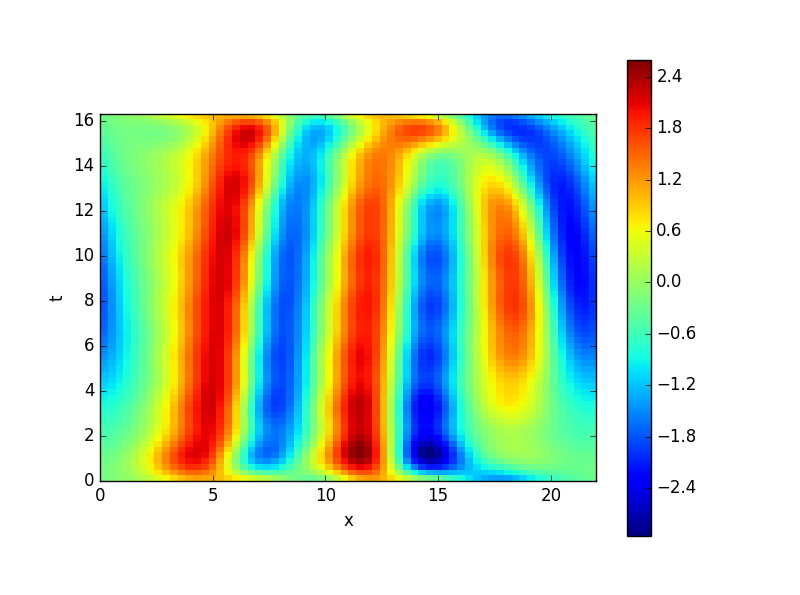
\includegraphics[width=\textwidth,height=.32\textheight]{MNGvndspaceinit2}
\end{minipage}
\begin{minipage}[height=.32\textheight]{.45\textwidth}
\centering \small{\texttt{(b)}}
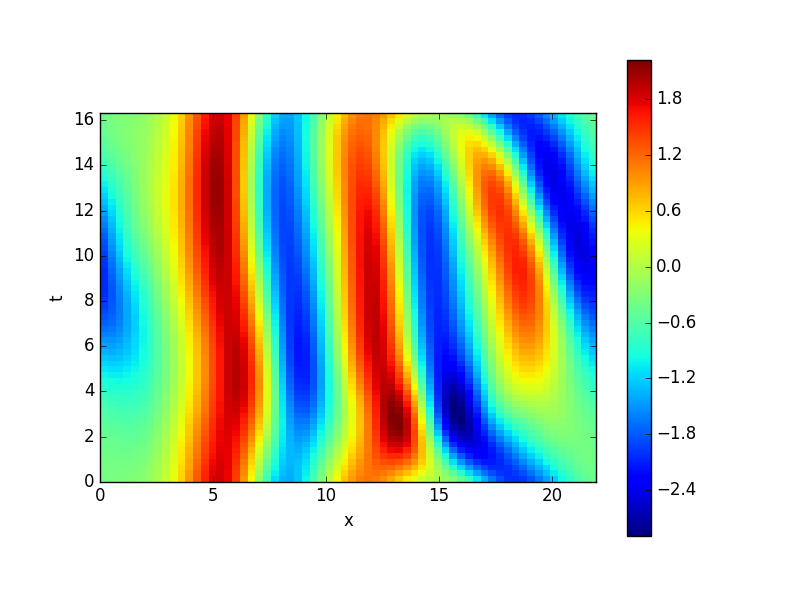
\includegraphics[width=\textwidth,height=.32\textheight]{MNGvndspacefinal2}
\end{minipage}
\caption{ \label{fig:MNGvndspace2}
(a) Initial condition of the 16-by-16 space-by-time discretization of \RPO{16.31} ($L=22$) for spatial
variational {\descent} of the \KSe\ (b)Resulting "spatial periodic orbit" (temporal equilibrium), with
final spatial extent of $L = 21.9394614064$
}
\end{figure}
\begin{figure}[ht]
\begin{minipage}[height=.32\textheight]{.45\textwidth}
\centering \small{\texttt{(a)}}
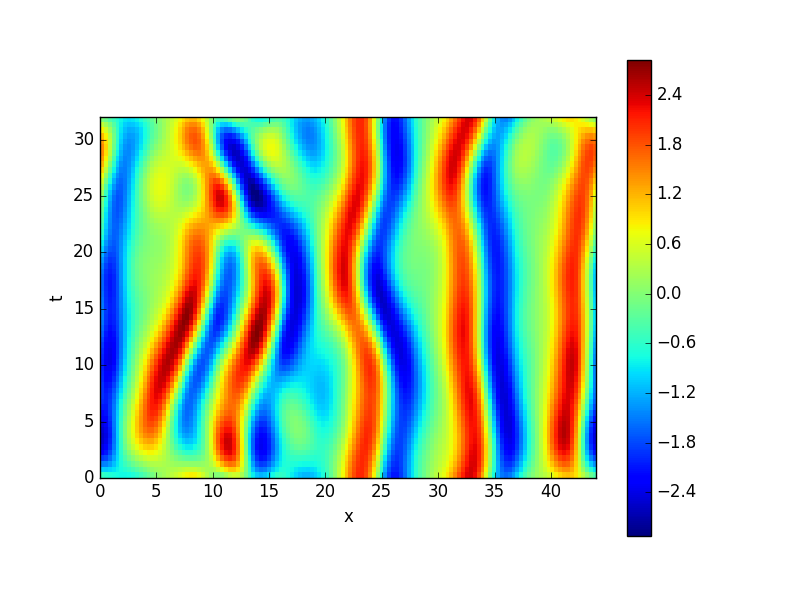
\includegraphics[width=\textwidth,height=.32\textheight]{MNGvndspaceinit3}
\end{minipage}
\begin{minipage}[height=.32\textheight]{.45\textwidth}
\centering \small{\texttt{(b)}}
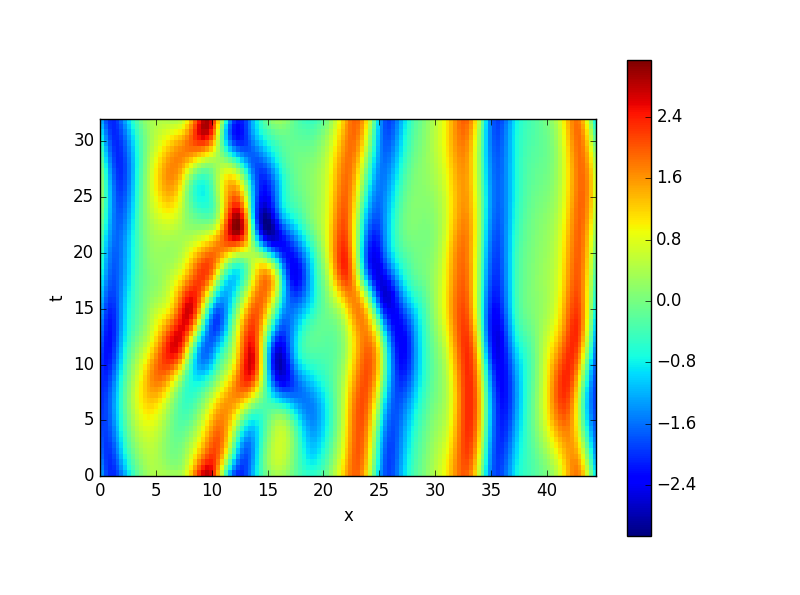
\includegraphics[width=\textwidth,height=.32\textheight]{MNGvndspacefinal3}
\end{minipage}
\caption{ \label{fig:MNGvndspace3}
(a) Initial condition of the 32-by-16 space-by-time discretization of a piece
of an ergodic trajectory that has been deformed to be periodic in time. $L=44$.
(b) Resulting spatiotemporal \po, with
final spatial extent of $L = 44.3937151766$.
}
\end{figure}


updated \reffig{fig:MNGvndspace2}, \reffig{fig:MNGvndspace1}, and uploaded \reffig{fig:MNGvndspace3} to display
current results.

After trying numerous small modifications to the variational method's system
of equations from \refref{LanThesis} including implementing factors involving
the coordinate involved in defining the in-slice time and other quantities
involving the slice tangents I didn't get any improvements over what I already
had. I still think the problem has to do with the slice time so I went over
the derivation of the equations and I believe I found a correction that can be
made.

The derivation of the system of equations used to find the fictitious time
corrections to the initial guess loop involves substitution of the
partial derivative of the rescaling factor with respect to fictitious time.
The way that this is done is via the definition

\beq
\lambda_n = \frac{\Delta t_n }{\Delta s_n} \, ,
\eeq
where, $s$ is the parameterization variable, here defined with a subscript $n$
to indicate that the parameterization need not be uniform around the initial guess
loop (although this is what I work worth as it makes things much easier to program).
$t$ in this instance stands for the real dynamical time of the orbit.

If we substitute the definition for the in-slice time, this equation takes the form

\beq
\lambda_n = \frac{\Delta \hat(t)_n (x_1)_n }{\Delta s_n}
\eeq

Going through the almost identical derivation for the system of equations there
is one place where I believe they differ. Normally, there is the substitution

\beq
\delta t_n = \frac{\partial \lambda_n}{\partial \tau} \Delta s_n \delta \tau
\eeq

Normally this is easily generalized in order to produce a uniform rescaling of the period
around the orbit,
but if the coordinate $x_1$ is involved I believe that this should take the form

\beq \label{e-inslicevarmeth}
\delta t_n = (\frac{\partial \lambda_n}{\partial \tau}(x_1)_n + \frac{\partial (x_1)_n}{\partial \tau} \lambda_n)\Delta s_n \delta \tau
\eeq

As the in-slice time rescaling is coordinate dependent, this formula seems to beg for a description
of the general equation that has a coordinate dependent rescaling. This is kind of what I have been stuck on
as this is quite different from what I am used to.

For a orbit that is described by $M$ points in time we would need ${\lambda_i}$ where $i = 0, ... , M-1$.
I'm currently working on implementing this into my current code but it's gotten the best of me so far.

The way I am attempting to solve the problem I am having with in-slice time is as such,
for $M$ discretized points representing an in-slice time description of a {\rpo} I am introducing
$M$ different time rescaling quantities $\lambda_m$. In this way the original variational
method equation changes from
\beq
\begin{bmatrix} D - \lambda diag(A_0, ... , A_{M-1}), & -v \end{bmatrix}
       \left[ \begin{array}{c} \delta \tilde{\conf} \\ \delta \lambda \end{array} \right] =
    \delta \tau \left[ \begin{array}{c} \lambda v - \tilde{v} \end{array} \right],
\eeq
to
\bea
&&\begin{bmatrix} D - diag(\lambda_0 * A_0, ... , \lambda_{M-1} * A_{M-1}), & -diag(v_0, ..., v_{M-1}) \end{bmatrix}  \left[ \begin{array}{c} \delta \tilde{\conf} \\ \delta \lambda_{m}
            \end{array} \right]
\continue
&&=
    \delta \tau \left[ \begin{array}{c} diag(\lambda_m) v - \tilde{v} \end{array} \right],
\eea
In this way the correction mentioned in \refeq{e-inslicevarmeth} is not being resolved but I want to try
to see if more flexibility in the rescaling of in-slice time with respect to fictitious time evolution
is sufficient before getting into an equation I derived; it's also a simpler step whose changes could be
carried over to the full in-slice time description I probably will need.

Wrote some new code for symmetry reduced spatiotemporal fixed point finding; currently
it seems a little strange to me because I only know how to quotient the spatial translation
symmetry in spatial Fourier space as opposed to spatiotemporal (double) Fourier space.

The way that this I am attempting this, are with the equations, in direct-matrix notation:

Using the definition of the reduced velocity in time, \refeq{e-KSsymDMvelnew}, restated here
for reference,
\beq
\hat{v} = (X \cdot \Fu) \ast v - (\dot{Y} \cdot v) \ast (I_M \otimes T) \cdot \Fu,
\eeq
We then find the equivalent spatiotemporal system by Fourier transforming in time by means
of application of $F_t$ linear operator denoting the transform and moving everything to one
side. Here, the $\Fu$ stands for a description of the initial solution that is only Fourier in space.
\beq
W\cdot F_t \cdot \Fu -F_t\cdot((X \cdot \Fu) \ast v - (\dot{Y} \cdot v) \ast (I_M \otimes T) \cdot \Fu) = 0
\eeq
The stability matrix resulting from this symmetry reduced mapping is therefore,

where $\hat{A}$ is in reference to the equation previously defined \refeq{e-KSsymDMstbnew}.

\beq
J = W\cdot F_t - F_t\cdot \hat{A}
\eeq

The part that troubled me for a while was how to implement symmetry reduction of the spatial translation
symmetry in a spatiotemporal way as opposed to what I have now. I haven't been able to come
up with anything good yet but it just seems like a little bit of a hack job to reduce
the symmetry before taking things to the spatiotemporal stage. Because I am trying
to find fixed points after symmetry reduction I imagined that this case should be
exactly be like symmetry reduction of a \reqva\ but I haven't found a good way of treating
the equations yet.

\section{gmres and iterative methods?}

Also, I still need to implement the Viswanath\rf{Visw07b} hookstep algorithm.

This ``residual vector" is sent to Arnoldi iteration in order to produce the
regular Hessenberg and Orthonormal matrices of this iterative procedure. In
between Arnoldi iterations, we check the new value of the residual, i.e.
$||b-A\delta\conf^{(k)}||$. If this meets a specific tolerance, it is then
passed to the least squares problem that defines GMRES\rf{Trefethen97}, find
y that minimizes $||H_n y - ||b|| e_1||$, this solution to the least squares
problem $y$ is then converted to Newton correction via multiplication of
orthonormal matrix $x = Q_n y$. If this Newton correction does not minimize
the residual sufficiently, GMRES is restarted. Until either a maximum
iteration number is met, or the relative differences between residuals stalls
out.

GMRES specific problems to take into consideration,
breakdown of the arnoldi iteration, if the test vector lies in the Krylov subspace,
then there will be a subdiagonal element of the
 Hessenberg matrix equal to zero (due to linear
  dependence and orthogonalization with
respect to the Krylov subspace). If this occurs then
 GMRES is restarted with another random test vector.
Numerically, this should be a condition on the value of the norm
of the vector being iterated upon.

In order to evaluate the matrix vector product $J \delta \conf$, the matrix-vector approximation previously discussed is used, where
we use $J\delta \conf \approx F(\conf +\delta \conf) - F(\conf) / \epsilon$, where $\epsilon = ||\delta \conf||$.

With what I have all reason to believe is a reasonable initial condition, a 64 by 64 discretization
of the first \ppo\ of \KS\ the initial value of the norm of the value of the mapping
$||F(u,T,L)||_2 \approx 10^-3$. I take this to be a good initial condition as the other values of norms
I have seen have had much higher initial values of this norm. The problem arises when I approximate
$J \delta \conf$. With almost any randomly generated $\delta \conf$, the norm of the vector $||J \delta \conf||_2
\approx F(u+\delta u, T + \delta T, L + \delta L) - F(u,T,L) / \epsilon $ with $||\delta \conf||_2 = \epsilon$.
yields a value that is dramatically larger than $||F(u,T,L)||_2$, and as such it does not allow for a convergent
Newton-Krylov search. The fact that the norm of the mapping of the spatiotemporal field is small, leads me to
believe that the code involving the mapping is correct, but if this is the case then the matrix-vector approximation
should be well written as well, as all it involves is this mapping function. It's this circular logic
with a hole in it that has been frustrating me to no end.

Something I can try is to use a second order approximation as opposed to a first order.
This would replace the approximate with $||J \delta \conf||_2
\approx F(u+\delta u, T + \delta T, L + \delta L) - F(u-\delta u,T - \delta T,L - \delta L) / \epsilon $

I thought it might be the form of the randomly generated perturbations that was possibly making things
go awry, as I believe it's logically justified to restrict perturbations such that the perturbed field would
yield a real field if transformed back into configuration space. I wasn't doing this before, but it seemed to
help my woes to a small extent, at least in terms of GMRES convergence; but again, in the scheme of things
it is a negligible benefit as the residual of the matrix-vector approximate far outstrips any change I
have made.

The second order finite difference approximation didn't really help the values I was getting from approximating
the \jacobianM\ so instead I tried to look for why the approximation seems so poor; I hadn't looked at the contributions
from the nonlinear and linear parts separately (I actually thought I did this a while ago but I think I had poor initial conditions
before). It turns out that the stiff components of the spatiotemporal mapping (i.e. high wavenumber modes due to the fourth power
of $q_k$) are what are contributing to the (what I consider too large) magnitude of the approximation the most.

I tried playing around with the perturbation magnitudes again, since it is mostly the high wavenumber modes contributing to the
magnitude of the approximate matrix-vector product I played around with having the perturbations to these modes be smaller in
magnitude than the rest, (i.e. some subset of the perturbations of the matrix of spatiotemporal Fourier coefficients is smaller in
magnitude than the lower (wavenumber, frequency number) modes). This didn't have enough of an effect so I instead started trying
to think of a way to justify a $2/3$ rule dealiasing (i.e. damping by setting equal to zero) of these contributions. This is
usually done during time-stepping, and is justified via an energy input argument. There is usually a contribution to the energy
of a solution due to aliasing and as such the higher modes are damped in any calculations in order to maintain energy-balance.

Also, the GMRES procedure is stalling out, so I have been looking towards ways to fix this. It seems that this is a relatively
well studied problem and the answer is to introduce preconditioning matrices into the GMRES scheme. This is done in a number
of ways and I have to find the best one for my problem, but I am also trying to find one that fits into my code already.
I think I will implement FGMRES, where the F stands for ``Flexible"\rf{Saad93}. It is called this because it
encourages the preconditioner to change at every outer-loop (Newton) step, while remaining the "same" for the inner-loop (arnoldi or GMRES)
steps. (same in quotes because at every iteration the rule to generate the preconditioner stays the same, but the matrix technically
changes in size).

I was being dumb with how I was creating the random perturbation vectors for my
GMRES procedure. After thinking about it a little more I realized I should just
create a random field of initial conditions in configuration space and then perform
a spatiotemporal Fourier transform to get the correct form of field. I can't explain
how much easier this is than what I was doing before. With this the stiff parts of the
linear portion of the mapping and as such I have returned the previous damping
of higher modes back to undamped status.
I've also been reading a bunch of
papers\rf{ChaJac84,Saad93,EldSim12,MoReHa14,LotYe05,GrGrReSz16,TBAMR92} on
preconditioning methods; and specifically for GMRES algorithm. It seems to be
a heuristic science much like taking Poincar\'e sections so I might have to
try a number of different preconditioners before I get one that works, or use
a combination of multiple different ones with different properties.
%    \PC{2017-05-02}{what is reference TBAMR92?}

It is reasonable
to take the zero vector to be the initial perturbation and begin arnoldi iteration
with the vector $-F(u) = b$, such that the Krylov subspace being generated through
GMRES is $K_n = <b, Ab, A^2b, ...>$.

Also I think I should be only using GMRES on half of the spectrum and such that there
are fewer variables in memory, and this way the structure of the Fourier coefficients
remains representative of a real valued velocity field when inverse Fourier transforms
are applied. I didn't do this until now because I didn't think it would be necessary
as I didn't see any mention of it in John's code but I think I should have known better
as this is what I have done in the variational codes at least.

Going to move on to preconditioners next, and I added (I believe up to the standards
of a decent human being modifying the bib file ) two more papers, \refref{Gijzen95,ReSaWo10} in this effort.
I am hoping to bridge the gap between these two with a hybrid method that uses the convenience of matrix-vector
products, the easily formed \jacobianM\ corresponding to the linear portion of the spatiotemporal mapping, and
preconditioning.

Rewrote functions in Newton-Krylov code to run with right-preconditioning
$J M (M^{-1} \delta \conf) = -F(x)$ with a Jacobi (approximate inverse of
\jacobianM\ based on diagonal elements) as a preconditioner, using the
hybrid finite-difference and explicit linear \jacobianM\ method I am trying and mentioned
in yesterday's blog post. Still have more
testing to do and the Jacobi preconditioner is usually not the best preconditioner from what
I have seen. Another common precondition uses the incomplete LU factorization
which I think I will try if it doesn't work.
Still have a couple more things to do before I can test properly but given
the prior difficulties I don't see things magically working out.

More work on torus code; After implementing my idea of defining
the nonlinear \jacobianM\ via finite-differences and the linear \jacobianM\
explicitly didn't work too well, I moved on to trying to see if doing everything
explicitly with use of SciPy's implementation of GMRES does the trick.

I didn't attempt this before because I was trying to explicit define \jacobianMs\
due to the memory usage but now considering I couldn't get the finite-difference
approximation to work (or maybe it's better to say that I don't think it's suited
for this problem) I decided to try doing everything explicitly, or at least
without using finite-differences

Xiong recommended using a Jacobi preconditioner (taking the inverse of the diagonal
elements of the \jacobianM) but I haven't had good results with this yet. I implemented
an ILU (incomplete LU factorization) preconditioner which approximates the inverse
of the entire \jacobianM, as opposed to only the diagonal elements. This worked better,
with Newton steps that actually reduced the residual and didn't send the period or length
to zero and or negative values. The only problem is that after a few
steps it would then fail to decrease the residual.
 I have a feeling this is an indication I am on the right
track but there are still some bugs to work out.
}

{\bf Matt 2017-04-10} ``the effect of changes
to the period and spatial size in expressions such as $F(u + \delta u , T +
\delta T, L + \delta L)$: [...]  why does it make
sense to take difference between two solutions where I am essentially
changing the domain size while keeping the discretization the same?''

{\bf Predrag} I do not think of it as subtracting domains of different sizes:
as far as the discretization is concerned, it is always the same $(N,M)$
discrete lattice, only the values of the field $u(x,t)$ on the lattice sites
are changing as you vary parameters $(L,\period{})$.

Look at the Fourier-discretized torus \refeq{e-FksSpattemp}. The
discretizations $(N,M)$ are the numbers of spatial, temporal Fourier modes
kept in the calculation. Clearly you can keep  $(N,M)$ constant while you
vary $(L,\period{})$ to $(L',\period{}')=(L+\delta L,\period{}+\delta\period{})$.
Spatiotemporal domain size $(L,\period{})$ enters only through the
parametrization
\(
q_k = {2 \pi k}/{L}
    \,,\;
\omega_\ell = {2 \pi \ell}/{\period{}}
\,.
\)

\section{spatiotemporal?}
While running other codes, I've been writing code that will solve the fixed point, i.e. algebraic
nonlinear equation that determines invariant tori.
Xiong lead me to look at L{\'o}pez \etal\rf{lop05rel}, which I took the time today to
read. I feel like it covers a lot of useful ideas and concepts that I will be
able to directly apply to my own problem. They use a numerical least squares
solver \texttt{lmder} to find fixed points, but I think it might be good to
invest time into implementing Newton-Krylov hookstep since J. Gibson holds it in
such high esteem. The general idea is to use a nonlinear solver to solve
\refeq{e-FksSpattempMat} augmented with a number of conditions for shifts and
periods such that the system is not underdetermined.

I'm currently working on something that I believe should work, which is to split
the \jacobianM\ into nonlinear and linear contributions; The normal equation that
arises is $J \delta u = -F(u)$. Due to the fact that I am looking for fixed points
this reduces to figuring out the kernel of the linear map defined by the \jacobianM.

There might be much more specifics in for this endeavor, but what I am planning
on doing is abusing the fixed point condition, splitting the \jacobianM\ into
an explicitly defined linear contribution, and an approximately defined (via
matrix-vector product approximation:
\(
J_{NL} \delta u = F(u + \delta u) - F(u)/ \epsilon
\,,
\)
where epsilon is a small (but not too small, as stated in
L{\'o}pez \etal\rf{lop05rel}), it should probably be around $\sqrt{\epsilon}_{machine}$ and
$\mathcal{O}(\epsilon) \approx \mathcal{O} \delta u$.

Then I would have a system of the form (L stands for linear, NL stands for nonlinear)
$J_L \delta u \approx - J_NL \delta u$, where I would be able to plug this system
into SciPy's GMRES function with $J_L = A, -J_NL \delta u = b$ and solve for x.

On these comments, the main references I have been studying are
\refrefs{lop05rel, KK04, BroSa90, ChaJac84}.

Rewrote lots of \texttt{MNGkstorifunc.py} as I've decided to abandon computing any \jacobianM\ explicitly
as the Matrix-vector approximation seems to be quite ubiquitous, and employed with Newton-Krylov methods it
is also known as Inexact Newton-Krylov as well as
\jacobianM-free Newton Krylov. This was somewhat hard of a decision to make as it meant I wasted some time
deriving explicit forms for the matrix elements of the \jacobianMs, but such is life.


I was hung up on how to actually compute these ``matrix-vector approximations"
in my context, after some exploring \refref{BoFra05, seg05, EshSle04}.
I think I've figured them out but I plan on talking to J. F. Gibson to confirm.
The other things I am trying to reconcile between the different notations is
how L{\'o}pez \etal\rf{lop05rel} handles symmetries of solutions as it's slightly different
than when one has a forward time mapping, I believe. These things and working in
the class objects I've defined in python turned out to be somewhat trickier
than I had first intended but I hope to get things up and running by the
weekend.

Also a note on symmetry, the way that J. Gibson
\HREF{www.channelflow.org}{(channelflow)} handles the spatial and temporal
translation symmetry is to constrain the Newton steps to only progress in
directions \PCedit{transverse to the spatial and temporal equivariance directions};
the idea is to use
additional equations of the currently underdetermined system of equations
(because we are keeping track of ``extra" variables: time and spatial periods,
spatial phase shifts from \rpo).

The additional equations that are tacked onto the Matrix-vector product approximation
of the \jacobianM\ are the inner products $( du, \frac{du}{dx} )$, $( du, \frac{du}{dL} )$, $( du, \frac{du}{dT} )$ in this
case. I am slightly worried that the galilean invariance will also make this more complicated; The reduction of the
galilean invariance in usually handled by setting the zeroth spatial Fourier coefficient equal to zero, but in this
two dimensional spectrum of Fourier coefficients this corresponds to a whole row of coefficients in the matrix
of coefficients equal to zero. In other words if the time series of these zeroth modes is always zero, then
the time Fourier transform of this information will also be identically zero.

The way I have it formulated right now is order to find roots $F(u,T,L) = 0$, I begin with the general formulation
of Newton's method for fixed points which (due to $F(x^*)$ equaling zero, with $x^*$ being the fixed point of this mapping, including
variations to period and spatial length of the system and any parameters that control other continuous symmetries.).
takes the form $J(x_N) \delta \conf_N = -F(x_N)$. Just to specify if the dimension of the {\statesp} (i.e. the number
of two dimensional Fourier coefficients) is $2MN$, where the factor of two is due to splitting the coefficients into
real and imaginary parts, then the vector $x^*$ is $2MN + 3$ (I think), due to freedom to change the period, length and
spatial phase. This is different than dealing with a symmetry reduced equations (which I feel like I should know is what I have
to do, but evidence in channelflow makes it seem like it is not necessary to find solutions).

You can think of the way it was traditionally done in continuing solutions.
First we fixed the spatial domain to a constant $L$, varied $\period{}$ to
$\period{}+\delta\period{}$ in order to find a spatiotemporally periodic
solution $u^{(1)}(x,t)$. Then we increased the spatial domain size $L$ to
$L+\delta L$, and used $u^{(1)}(x,t)$ (the same $N$ Fourier modes) as a
starting guess, varied $\period{}$ to $\period{}+\delta\period{}$ and
determines the spatiotemporally periodic solution $u^{(2)}(x,t)$,
parametrized by $(L+\delta L,\period{}+\delta\period{})$.

But this traditional continuation is like having a function $F(x_1,x_2,x_3)$
which happens to have zeros lying on a curve in 3-space, fixing $(x_2,x_3)$,
using 1D Newton to determine $x_1$, then changing $x_2$ to $x_2+\delta x_2$,
using 1D Newton to determine the new $x_1$, \etc. Clearly not smart, you want
to use the 3D Newton instead. As solutions are not isolated --they lie on a
curve-- you need some extra condition to parametrize them along the curve. Could
be $L$ or $T$, but we should probably think of something smarter, like the
energy of the solution.
}

If this doesn't work I think I will attempt an even simpler problem, i.e.
the two modes problem as per Burak's recommendation; much like how I started
with the R\"ossler system for the variational method.
A quick computation of the condition number of the explicitly defined \jacobianM\ using
singular value decomposition reveals that it's in the tens of millions, which I believe
proves that I am dealing with a highly ill-conditioned system of equations.
By disabling changes to the period and length of the system this is lowered by an
order of magnitude, however, I believe this still implies that the system is highly ill-conditioned
even when trying to find fixed points of the spatiotemporal mapping on a fixed spatiotemporal domain.
Xiong suggested that perhaps I can use the singular values to produce a preconditioner that might help,
I'm looking into this as well as some other papers\rf{Meza95}

Today's dealings mainly involved working through the "direct matrix method" in \refref{Chu09}.
The reasons why I opted to rewrite my code in this way are: I feel like it is less
prone to errors than index notation, it agrees with how I think about things, as it
very much resembles \refeq{e-FksSpattempMat}, something that I worked through myself.
The basis of the method is to rewrite everything into either component-wise products
(also known as, entrywise product, hadamard product,
schur product)  or matrix multiplications. In this form, the spatiotemporal mapping is given explicitly
by the following equation. Note that $\star$ implies component wise products (saves computing time versus
matrix-vector products with diagonal matrices and a vector) and $(\dot)$ implies matrix multiplication. $\Fu$
from here on is going to be a vector $\in \mathcal{R}^{MN}$ where $M$ is number of discretized points in time and $N$ is
the number of discretized points in space. In practice, due to the symmetries of the problem, (galilean invariance, real valued
velocity field implies a symmetry in the spatiotemporal Fourier coefficients), $\Fu \in \mathcal{R}^{mn}$ where
$m = M-1$ and $n = N/2 - 1 $. (I could have likewise chosen $m = M/2 -1$ and $n = N-1$ if so desired.) In this formulation,
the Fourier coefficients kept $(\tilde{u}_{k \ell})$ pertain to values of indices $k = 1, 2, \ldots, N/2-1$ and $\ell = 0,1, ...
M/2-1, -M/2+1, \ldots, -1$ (Nyquist frequency removed, $l = M/2$).
As will be seen, this makes the formulation of the matrices corresponding to Fourier transforms, also known as "DFT matrices",
rectangular; but I made sure the matrix multiplications are well defined if defined correctly. One might argue that making
this change is undesirable due to the number of operations of matrix multiplication, but I feel like it will be competitive
once I do the calculations on how many operations are gained or lost.
For the time being I formulating this method to fix $T$ and $L$; this \emph{should} be
an easy addition afterwards.

\beq \label{e-FksMatrix}
(Q_1 \star \Fu) + (W \dot \Fu) + Q_2 \dot F \dot ((F^{-1} \dot \Fu) \star (F^{-1}\dot \Fu))
\eeq

With the definition of the spatiotemporal mapping in place, it is convenient to now describe the "direct-matrix calculus"
operations as defined in \refref{Chu09}

For arbitrary matrices $A$, functions of $\Fu$, $F(\Fu), G(\Fu)$, the rules for differentiation are as follows,
(note asterisks indicate component wise multiplication and dots indicate matrix multiplication.)

\beq \label{e-DMdiffrules}
\frac{\partial}{\partial \Fu}(A \cdot \Fu) = A
\eeq

\beq
\frac{\partial}{\partial \Fu}(F(\Fu) \ast G(\Fu)) = diag(G(\Fu)) \ast \frac{ \partial F(\Fu) }{ \partial \Fu } + diag(F(\Fu)) \ast \frac{ \partial G(\Fu) }{ \partial \Fu}
\eeq

\beq
\frac{\partial}{\partial \Fu} = A \cdot \frac{ \partial F(\Fu) }{ \partial \Fu }
\eeq


With the use of these identities, I find the the form of the \jacobianM\ as,

\beq
J = W + Q_1 + Q_2 \cdot F \cdot diag(F^{-1} \ast \Fu) \cdot F^{-1}
\eeq

In order to exploit the matrix vector notation, I construct matrices that would apply element-wise multiplication
of powers of $q_k$ and $\omega_\ell$ to the spectral grid at fixed $k$ and ranging $\ell$ (or vice-versa) and then
exploit Kronecker products to form a matrix that applies this multiplication over all indices.

For a quick example, a diagonal matrix whose diagonal elements equal $-q_k^2 + q_k^4$ is made, and then a right-hand
Kronecker product is taken such that the final matrix is of size $(mn)^2$ (note: small letters represent reduced dimensionality
due to symmetry of Fourier coefficients). I.e. it is a matrix whose diagonal contains $m$ copies of the elements of
the vector of length n whose elements equal $-q_k^2 + q_k^4$.

Because we also want to split into real and imaginary parts, this is actually done twice, such that the final matrix diagonal
is two copies of the diagonal of the matrix of size $(mn)^2$. In this manner, we can correctly apply the operation of multiplication
by $-q_k^2 + q_k^4$ to a vector whose elements equal ${a_{kl}, b_{kl}}$ where $a_{kl},b_{kl} = Real[\Fu_{kl}], Imag[\Fu_{kl}]$.
Note, due to the how python arranges indices upon reshaping of arrays, the second index $\ell$ is the "inner" index, what I mean by this
is that all values of $\ell$ are cycled through, at which time the "outer" index $k$ is cycled once. Also, the vector is formatted
such that all real parts of the coefficients are cycled through before reaching the imaginary parts of the coefficients.

The definitions of the matrices are as follows,

\beq \label{e-MNGwoperator}
\begin{bmatrix}
W = 0 & -\omega_\ell \\
    \omega_\ell & 0
\end{bmatrix}
\eeq

\beq \label{e-MNGq1operator}
\begin{bmatrix}
Q_1 = -q_k^2 + q_k^4 & 0 \\
    0 & -q_k^2 + q_k^4
\end{bmatrix}
\eeq

\beq \label{e-MNGq2operator}
\begin{bmatrix}
Q_2 = 0 & -q_k / 2 \\
    q_k / 2 & 0
\end{bmatrix}
\eeq

The matrices governing the forward and backward inverse transforms are confusing and I don't think will be
well elucidated when written in equation form, therefore, I will try to explain them. With the forward
two dimensional discrete Fourier transform defined as $F = F_T \cdot F_X$.

$F_X$ is a matrix of shape
$2\,M\,n \times M\,N$, which is produced by taking the real-valued FFT of the identity $\mathcal{I}_N$, and
deleting the first and last rows (this is due to symmetries in the Fourier coefficients), after some reordering
of the rows (due to discrepancies of scipy convention and how I would like to order my {\statesp} vectors),
a right-hand Kronecker product is taken with the identity $\mathcal{I}_M$.

$F_T$ is a matrix of shape $2*m*n \times 2 * M *n $ which is produced by taking the regular(complex) FFT on the
identity $\mathcal{I}_M$, at which point the row corresponding to $\ell = M/2$ is removed. Because the {\statesp} vector is split into real and imaginary parts at this point (due to the real valued fft applied by $F_X$,
we must split the real and imaginary components of the current matrix into blocks, such that this matrix is
also real valued.

That being said, this is almost the entire code so I still haven't completed it. The trickiest part is the matrices
representing Fourier transforms. Note: I am only deleting rows and columns
that would correspond to zero-valued Fourier coefficients,
so I should not be losing any information in the process. That being said, there is a small error somewhere that
I haven't been able to find that is preventing the operation of $F^{-1} \cdot F$ from equalling the identity.

Added code to enables varying period and spatial dimension of the spatiotemporal
Newton's method code. It converges to within machine precision, however, there is a
slight problem that I've been trying to hunt down. For the initial condition that
I described in the prior posts, my spatiotemporal fishnet stocking (or two dimensional
spectral grid), the period ends up being stretched by a large factor, the spatial size
shrinks, and the spatiotemporal Fourier coefficients shrink to the equilibrium solution $u=0$.

In the past with my variational code this usually implied bad constraint equations, or a small
numerical error somewhere in the code. (i.e. a factor of two as was the case for the variational
code.) I spent the remainder of the day hunting for errors but haven't found any so far. To be honest,
I am again encouraged just by the fact that the full problem is at least converging to something, even
if it is a horrible numerical result.

I'm looking into other constraints that I could possibly implement to hope to settle this once and
for all. It might just be that these constraints work better for GMRES versus linear solvers based
on LAPACK, I'm not sure right now.
In order to avoid headaches with constraints, I chose the easy road which was to use a least
squares (pseudoinverse) solver as opposed to the solver I was using.
This dramatically changed the behavior of corrections to the period and spatial size of the
system, but sadly, the initial condition I used still went to the trivial equilibrium. I am
going to try to improve the initial condition I am using as the initial residual is relatively
large, so it could just be a mistake in the initial condition generation. Going to test
on other equilibria and see what comes out from the black box.


\begin{figure}[ht]
\begin{minipage}[height=.32\textheight]{.45\textwidth}
\centering \small{\texttt{(a)}}
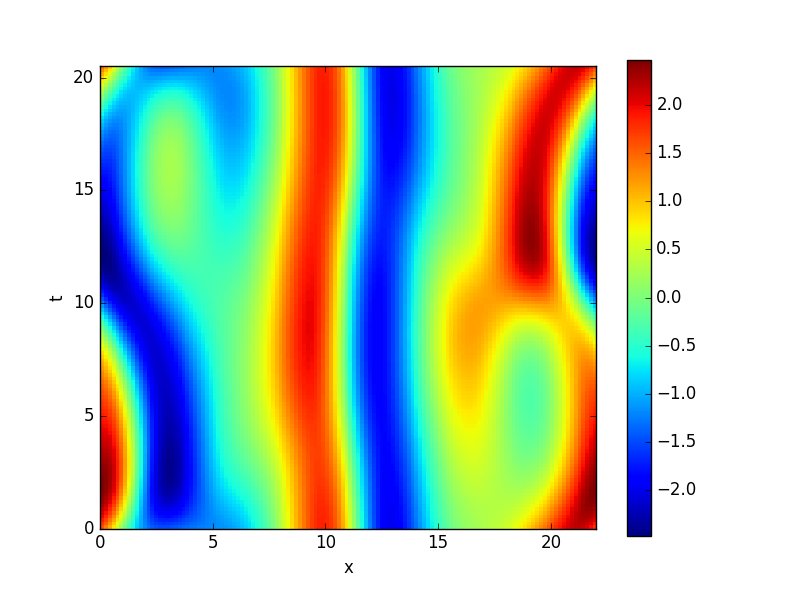
\includegraphics[width=\textwidth,height=.32\textheight]{MNGspacetimeinit1}
\end{minipage}
\begin{minipage}[height=.32\textheight]{.45\textwidth}
\centering \small{\texttt{(b)}}
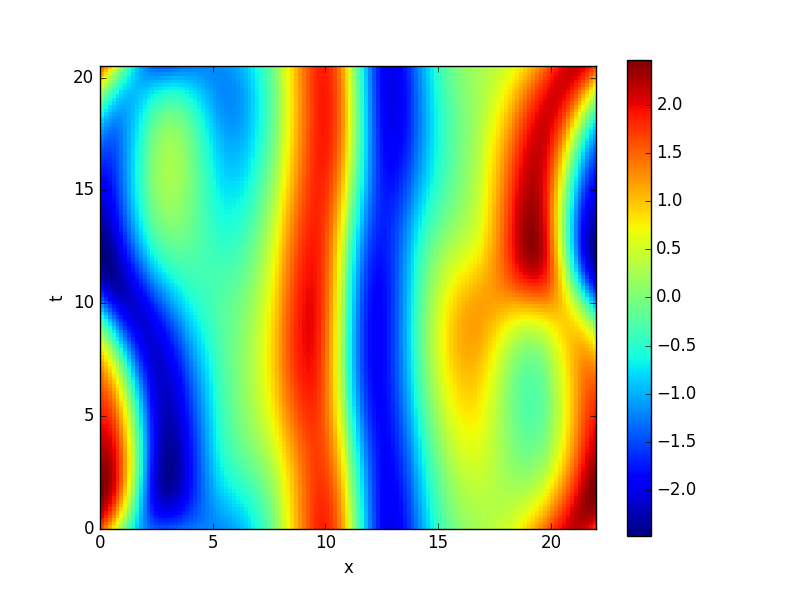
\includegraphics[width=\textwidth,height=.32\textheight]{MNGspacetimefinal1}
\end{minipage}
\caption{ \label{fig:MNGspacetime11}
(a) Initial condition of the 32-by-32 space-by-time discretization of \PPO{10.2}:
$(L_0,\period{0}) = (L_0, 2\period{p_0})= (22,20.5057459345)$.
(b) Resulting spatiotemporal fixed point
$(L_p,2\period{p}) =  (22.0000104401, 20.5057499188)$
}
\end{figure}

\begin{figure}
\begin{minipage}[height=.32\textheight]{.45\textwidth}
\centering \small{\texttt{(a)}}
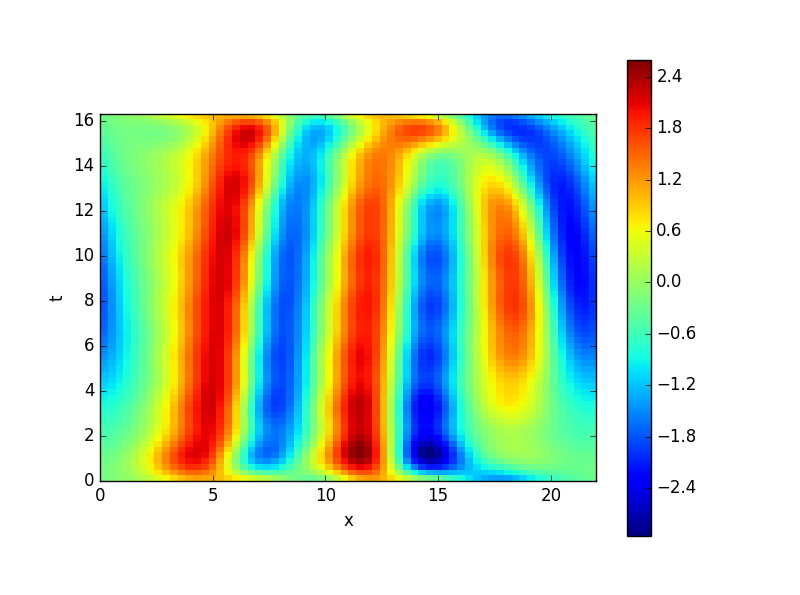
\includegraphics[width=\textwidth,height=.32\textheight]{MNGvndspaceinit2}
\end{minipage}
\\
\begin{minipage}[height=.32\textheight]{.45\textwidth}
\centering \small{\texttt{(b)}}
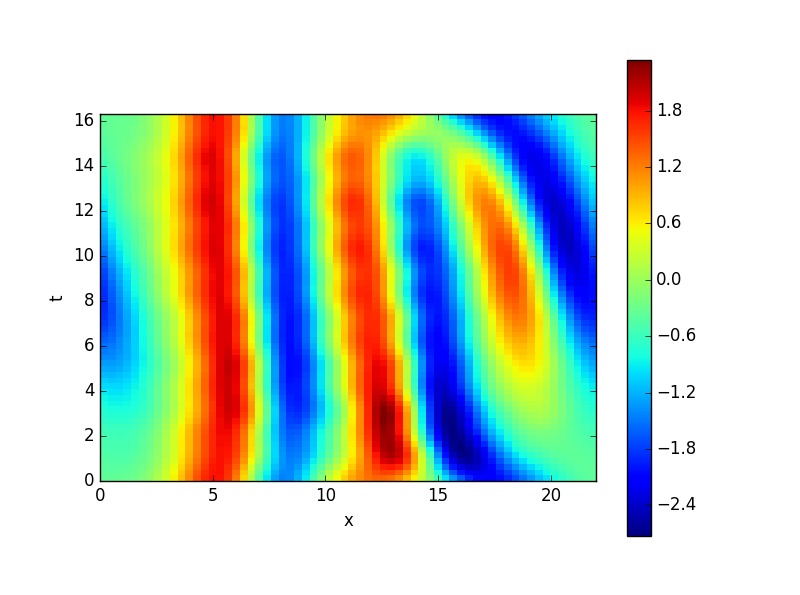
\includegraphics[width=\textwidth,height=.32\textheight]{MNGvndtimefinal2}
\end{minipage}
\begin{minipage}[height=.32\textheight]{.45\textwidth}
\centering \small{\texttt{(c)}}
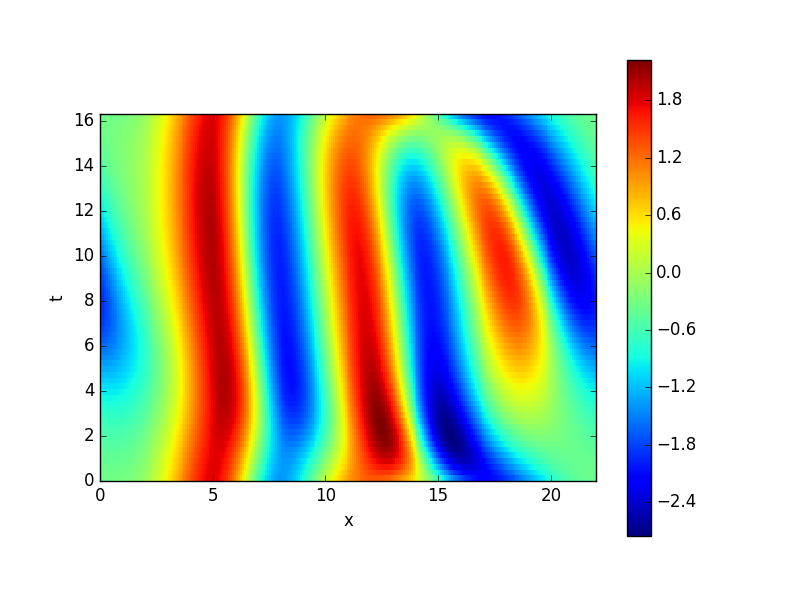
\includegraphics[width=\textwidth,height=.32\textheight]{MNGvndspacefinal2L}
\end{minipage}
\caption{ \label{fig:MNGspaceandtime1}
(a) Initial condition of the 16-by-16 space-by-time discretization of
\RPO{16.31}. $L_0 = 22$.
(b) Resulting periodic orbit after variational {\descent} in time $L =
22, T = 15.7444884386$,
(c) resulting periodic orbit after variational {\descent} in space.
%%%lost the number for final spatial size will need to run code again.
}
\end{figure}

As a means of cross-checking results I wrote variational {\descent} code for time, debugged, and got it working. It follows the "direct-matrix" approach
that I have been finding useful.
The velocity equation takes the form
\beq \label{e-MNGkstimeDM}
v = Q_1 \cdot \Fu - Q_2 \cdot F \cdot ((F^{-1}\Fu) \star (F^{-1}\Fu))
\eeq
and the stability matrix is therefore
\beq
A = Q_1 - 2 * Q_2 * \cdot F \cdot diag(F^{-1}\Fu) \cdot F^{-1}
\eeq

\reffig{fig:MNGspaceandtime1} is a comparison between resulting orbits from both space and time variational {\descent}.
The general structure of the resulting orbit is preserved even though the periods are quite different. At first I believed that
these were supporting evidence that something is going right but now I am confused. The spatial domain resulting from the \emph{spatial}
{\descent} is largely unchanged, meaning that the orbit that results should be a unique solution with a unique period; but the \emph{time}
variational {\descent} changes the period somewhat drastically, and because the spatial domain size is fixed this might mean that I am
finding the same solution but this is contradictory because the periods are so different. Also good evidence that there is something wrong is that
the \emph{time} {\descent} is taking a \rpo\ initial condition and seemingly changing it into a periodic orbit? I don't know what
to think of it but I am glad that I rewrote the time {\descent} code as it'll be a good stepping stone into whether or not I need to rewrite the equations
in a symmetry reduced form in order to find {\rpo}s or not. I think that's where I'm headed at least.

Firstly, we must generate symmetry reduced spatiotemporal initial conditions, this, plainly, is done by
using a symmetry reduced time integrator such as Burak's \texttt{ksETDRK4red.m} to generate a spatiotemporal
discretization that will be used for the hunt.

Next, I rewrite the direct-matrix equations in a symmetry reduced form. I find it easiest to first
look at the symmetry reduced velocity equations for \KSe\ and then figure out what is necessary to take
the leap into turning them into a spatiotemporal mapping such as \refeq{e-FksSpattemp}.

Taking equations (8),(9) from \refref{BudCvi14}, the symmetry reduced flow takes the form
\bea
    \hat{v}(\hat{a}) &=&
                v(\hat{a}) - \dot{\theta}(\hat{a})t(\hat{a}) \,, \quad
    \dot{\theta}(\hat{a}) =
                \frac{\langle v(\hat{a}) | t'(\hat{a}) \rangle}{\langle t(\hat{a}) | t'(\hat{a}) \rangle} t(\hat{a})    \,, \quad
    \label{e-symred}
\eea

Now, in order to put this symmetry reduced flow
into a spatiotemporal setting, where the entire orbit is then treated as a vector in the domain the spatiotemporal mapping,
we must make note that for the $N-by-M$ discretizations that we are going to use in the fixed point finder
we need to expand these formulae to account for the fact that we need $M$ copies of the template vector $t(\hat{a})$ for every
point in time; likewise in order to evaluate the group tangent of at for the $2NM$
dimensional vector (2 because of Fourier)
we need to take a Kronecker product between the identity and the \SOn{2} generator in order to have a
$[2NM\!\times\!by-2NM]$ matrix that
will produce the correct group tangent after multiplication with the spatiotemporal vector.

Now once we have all of these things in place we can produce an equation similar to \refeq{e-FksSpattempMat} for the
symmetry reduced flow. Substituting $v$ from \refeq{e-MNGkstimeDM},
(the transparency) the symmetry reduced flow can be written as
\beq
\hat{v}(\hat{a})= \frac{\partial a}{\partial \tau} = f(a),
\eeq
where $\tau$ is the in-slice time.

Then applying an operator $F_t$ that takes the temporal Fourier transform around the orbit, and rewriting the time-derivative
by exploiting the Fourier transform we are left with
\beq
W_{\tau}*\hat{u} - F_{\tau} \cdot f(\hat{a}) = 0
\eeq
Now, for the record, I write the equation in its complete
direct-matrix, symmetry reduced form.
\bea
0 &=&
W_{\tau}*\hat{u}
- F_t ( Q_1 \cdot \Fu - Q_2 \cdot F \cdot ((F^{-1}\Fu) \star (F^{-1}\Fu))
    \ceq
- \frac{\langle Q_1 \cdot \Fu - Q_2 \cdot F \cdot ((F^{-1}\Fu) \star (F^{-1}\Fu)) | t'(\hat{a}) \rangle}
       {\langle t(\hat{a}) | t'(\hat{a}) \rangle} t(\hat{a}))
\eea
where $\Fu$ is now the vector quantity that completely describes the spatiotemporal symmetry reduced orbit in question.

Note: the definitions of the operators before taking Kronecker products are from \refeq{e-MNGwoperator}, \refeq{e-MNGq1operator}, \refeq{e-MNGq2operator}.

Finding some better numerical results with the alternate definitions for
\refeq{e-symred} which are, ($x_i$ implying real part of $i$th Fourier mode,
$y_i$ is the imaginary part, where $i = 1, ..., N/2-1$

\bea
    \frac{\partial \hat{a}}{\partial \tau} &=&
                \hat{x}_1 v(\hat{a}) - \dot{y}_1(\hat{a}) t(\hat{a}) \,, \quad
    \frac{\partial \theta(\hat{a})}{\partial \tau} = \dot{y}_1(\hat{a})
                   \,, \quad
    \label{e-symred2}
\eea

I believe that the stability matrix with take the following form,
\beq
\hat{A} = diag(x_1)\cdot A - diag(\dot{y}_1(\hat{a}))\cdot T
\eeq


Finished implementing the newer version of symmetry reduction variational method
\refeq{e-symred2}.
Still having issues as initial condition for the value of the cost-functional, which
is the best indication I have that I am still somehow messing up the symmetry reduced equations;
the only other contributor could be the approximate loop tangent, which I realized today
should also be symmetry reduced, i.e. it doesn't make sense to compare the in-slice velocity
to an \MNGedit{approximations of element in the full {\statesp} tangent bundle}.

After being frustrated for a while I finally realized the dumb mistake I have been making
when it comes to symmetry reduction. I have been trying to compute the symmetry reduced
velocity at every point of the discretized symmetry reduced {\rpo}s all at once. This was
the wrong choice because the equations rely on inner products of vectors specific to each point
along the discretization (namely the full \statesp\ velocity and the group tangents at
the slice template point and each time discretization point).

I don't know why I didn't realize this before (I guess I'm learning?) but something clicked
when I noticed that the wrong elements were being set to zero in my previous formulation, in other
words the in-slice symmetry reduced velocity wasn't tangent to the slice.
I tested out the formulae I have been using for a single point along the discretization in time and everything resolved.

In more detail, previously I was using a template point that was the same dimension as the entire discretized
orbit, i.e. for an $N-by-M$ space-by-time discretization of an \rpo\ I was using $M$ copies
of the same template vector expecting it to work but this is fundamentally flawed because
when I use the equations \refeq{e-symred} all this does is mix all of the information of
the orbit together in a jumbled fashion that makes absolutely no sense.

If I can't figure out a way then there is the back-up
plan of performing operations one at a time (as opposed to using
linear operators that act on the entire discretized orbit at once)
by computing the symmetry reduced velocity of each \statesp\ point and each symmetry reduced
stability matrix one by one and then compiling them respectively into the vector, matrix that I need:
A vector containing the in-slice velocities at every point along the orbit and a block
diagonal matrix whose blocks are comprised of in-slice stability matrices evaluated as the
respective point along the orbit.

After I posted yesterday I almost immediately figured out the issue with the current formulation and why it won't work. It's a matter
of the ordering of the variables; the way I have the code currently written the variables are ordered in a spatiotemporal vector
that cycles through the time first and then space. I.e. if $k$ and $\ell$ were indices that take values from $0, \cdots, N-1$
and $0, \cdots, M-1$ respectively representing the the space and time discretization, for every unit change to $k$, the index
$\ell$ would have cycled through $M$ values.

Now, this isn't important it's just a clerical part of coding but the problem I am now facing is that this specific ordering
is going to make it much harder to finish the symmetry reduction variational code. I've tried to work things out
in a number of ways but they are require some very unintuitive measures that I feel would be best to avoid. So, for now,
I am going to rewrite everything such that the ordering of the \statesp\ vector cycles through spatial indices first, in other
words switching to a different standard.

With this in mind, I believe I have a way to rewrite \refeq{e-symred} such that it will serve my purposes of symmetry reduction.
Like I've said before the problem I had from a lack of practice was that I was trying to symmetry reduce the entire orbit at
once not taking into consideration that the group tangent direction (amongst other things) is a time-dependent quantity.

Here is how I believe I can fix things once I change the ordering of the spatiotemporal vector i.e. the orbit in vector form.
It basically relies on computing $M$ copies of \refeq{e-symred} while keeping all of the information at different times separate.
Starting with,
\bea \nonumber
    \hat{v}(\hat{a}) &=&
                v(\hat{a}) - \dot{\theta}(\hat{a})t(\hat{a}) \,, \quad
    \dot{\theta}(\hat{a}) =
                \frac{\langle v(\hat{a}) | t'(\hat{a}) \rangle}{\langle t(\hat{a}) | t'(\hat{a}) \rangle} t(\hat{a})    \,, \quad
\eea

Let $v$ now be matrix whose rows (instead of columns as to reshape the matrix into a vector properly)
are the full \statesp\ velocity evaluated along the time discretization of a symmetry reduced
\rpo. Likewise, define $\hat{a}$ as a matrix whose rows are the current (in fictitious time) representation of the symmetry
reduced \statesp\ points that comprise the \rpo. Then, we can change the inner product notation to a matrix-vector product notation
by virtue of the group tangent template vector being constant. For example, the velocity will now be concatenated in a matrix
in the following manner.

\beq
v(\hat{a}) \rightarrow \mathbf{V} \equiv [v(\hat{a}(\tau_0)) | v(\hat{a}(\tau_1)) | \cdots | v(\hat{a}(\tau_{M-1})) ]
\eeq

following this notation the equation for evaluating the symmetry reduced velocity at every point along our discretization
will be

\bea \nonumber
    \hat{\mathbf{V}}^T(\hat{a}) &=&
                \mathbf{V}^T(\hat{a}) - \dot{\theta}(\hat{a}) \mathbf{t}^T(\hat{a}) \,, \quad
    \dot{\mathbf{\theta}}(\hat{a}) =
                (\mathbf{V}^T(\hat{a}) \cdot t'(\hat{a})*/ \mathbf{t}^T(\hat{a}) \cdot t'(\hat{a})) \mathbf{t}^T(\hat{a})  \,, \quad
\eea

Now the onto the stability matrix; as opposed to the symmetry reduced velocity where
I can just concatenate vectors into matrix and perform element-wise operations and matrix-vector products, with the stability
matrices I needed to rewrite definitions of all of the matrices involved in the direct-matrix derivation which I am
still in the process of. Some of them are easy, where the effect of the reordering merely results in the opposite order
kronecker product.

Wrote code to produce more general initial conditions for symmetry reduced variational methods.
Alright. I have mostly figured out the issues. I guess I was confused on how to use the in-slice time symmetry reduced
velocity in conjunction with the direct-matrix formulation before. I was attempting to use equations \refeq{e-symred}
in place
of something similar to \refeq{e-symred2} and this was a tragic mistake that took me a week to figure out.

The following are what I believe to be the correct implementation of symmetry reduction for the variational
method when applied to a {\rpo} that has been generated with a symmetry reduced integrator. In other words,
when the initial condition is a spatiotemporal discretization embedded in the slice

The new equation I am using for calculation of the symmetry reduced velocities (w.r.t. in-slice time) in the
direct-matrix formulation is,
\beq \label{e-KSsymDMvel}
\hat{v} = (diag(x_1(t)) \otimes I_{N-2})\cdot v - (diag(\dot{y}_1(t)) \otimes I_{N-2}) \cdot (I_M \otimes T) \cdot \Fu
\eeq

This is relatively simple to explain when using \refeq{e-symred2} as a reference. $diag(a_1(t))$ is a diagonal
matrix that when multiplied with the full \statesp\ velocity vector produces a vector whose entries
are equal to $x_1(t_i)*v(t_i)$ where $x_1$ is the real component of the first Fourier mode. likewise for $diag(\dot{y}_1(t))$
except $\dot{y}_1$ is the velocity of the imaginary component of the first Fourier mode. the $\otimes$ symbol here
denotes a Kronecker product (outer product) whose purpose is to copy the values $x_1$ and $y_1$ as to create a diagonal
matrix whose dimension equals the dimension of the velocity vector $v$. i.e. I need an outer product with a $N-2$ identity
matrix to ensure that I have $N-2$ copies of $x_1$ and $y_1$ so that each of the $N-2$ Fourier modes gets multiplied by
the correct factor.

To simplify the notation and make it more apparent how to derive the stability matrix in direct-matrix notation, I rewrite
$X_1 = diag(x_1(t)) \otimes I_{N-2}$ and $Y_1 = diag(\dot{y}_1(t)) \otimes I_{N-2}$.

The equation for the stability matrix for the entire orbit is therefore.

\beq \label{e-KSsymDMstb}
\frac{\partial \hat{v}}{\partial \Fu} = \hat{A} = X_1 \cdot A - Y_1 \cdot T
\eeq

I believe it might be that I have treated $X_1$ and $Y_1$ as constant matrices as opposed to functions of $\Fu$. This
is the only place that I find room for errors so far.

Small progress on symmetry reduced variational methods front. With some small changes to how I implemented
\label{e-KSsymDM0}. and playing around
with different discretizations of \RPO{16.3} I was able to get a final result whose value
of the cost functional is $F^2 \approx 10^{-12}$. This is four orders of magnitude of improvement
from the initial value of $F^2 \approx 10^{-8}$ but it's still not good enough.

The new formulations of \refeq{e-KSsymDMvel} and \refeq{e-KSsymDMstb} are written in the following ways, to more
explicitly represent the dependence of the matrices $X$ and $Y$ on the underlying quantities, namely the
orbit vector (vector representing the time discretizations of the spatial Fourier series)
and the full {\statesp} velocity vector.

\beq \label{e-KSsymDMvelnew}
\hat{v} = (X \cdot \Fu) \ast v - (\dot{Y} \cdot v) \ast (I_M \otimes T) \cdot \Fu
\eeq

with this (more) correct direct-matrix velocity equation we can then derive the corresponding stability matrix,
using the rules of calculus described in \refref{Chu09}

\beq \label{e-KSsymDMstbnew}
\frac{\partial \hat{v}}{\partial \Fu} = \hat{A} = diag(v)\cdot X + diag(X \cdot \Fu )\cdot A - diag(T \cdot \Fu)\cdot (Y \cdot A) - diag(Y \cdot v)\cdot T
\eeq

The new formulation helped me find an error in how I was deriving the stability matrix as there was dependence on
both the orbit vector $\Fu$ and velocity vector $v$ in the matrices $X_1$ and $Y_1$ in \refeq{e-KSsymDMstb} that
I was not accounting for.



Made some changes that make the problem seem more natural, namely, I included some terms such that everything
is in terms of linear operators acting on vectors of spatiotemporal Fourier coefficients as opposed
to a weird mixture I had before. The upside is that everything is defined spatiotemporally, but it might
look a little odd at first glance because there are certain terms which only have one type of Fourier transform operator being applied.

I also elected to change the temporal Fourier transform to a RFFT based description as opposed to a FFT
based description (FFT produces both sides of the spectrum, negative and positive Fourier modes based on index
where RFFT just produces half of the spectrum). I avoided this earlier because it was easier at first but
now that I have some experience this RFFT based description is definitely desired as it minimizes the number
of variables in the system. (It is possible, of course to take a FFT and then keep half of the terms but
this would be hard to implement given my direct-matrix implementation). The problem isn't completely
symmetric in terms of space and time however, as the Galilean invariance eliminates the need to keep
track of the terms corresponding to zeroth and Nyquist $(N/2)$ modes of the spatial spectrum; The easiest
way to describe this is that the discretization in spatiotemporal Fourier space is $N-2 by M$ where $N$
is the spatial discretization and $M$ is the temporal discretization.


The mapping now takes the form,
\beq \label{e-symredmapping}
W\cdot \Fu -F_t\cdot((X \cdot F_t^{-1} \Fu) \ast v - (\dot{Y} \cdot v) \ast (I_M \otimes T) \cdot F_t^{-1} \cdot \Fu) = 0
\eeq
where, $\Fu$ denotes a vector of spatiotemporal Fourier coefficients.

The symmetry reduced stability matrix needed for Newton's method then takes the form
\bea
M &=& W - F_t [diag(X \cdot F_t^{-1} \cdot \Fu)\cdot A - diag(v)\cdot(X\cdot F_t^{-1})
    \ceq
+ diag(Y\cdot v) \cdot (T \cdot F_t^{-1})
+ diag(T\cdot F_t^{-1} \cdot \Fu) \cdot (Y\cdot A)]
\eea
This is in addition to the partial derivatives with respect to in-slice time
and domain size that have yet to be elucidated.

I have been thinking for a while when this works how I will begin to apply it to glue different orbits together,
but finding {\rpo}s in a symmetry reduced space and {\ppo}s in full {\statesp} can't really be stuck together
in my mind so I think the correct way would be to find the {\rpo}s in reduced {\statesp}, reproduce
them in full {\statesp} through numerical integration and then try to glue them together. This wouldn't
warrant a further attempt to find another spatiotemporal fixed point however because the \rpo\ in full
{\statesp} through one prime period would not be periodic in time, but it would be periodic in space.
There a couple of thoughts I have had about this, one being that perhaps maybe when looking at the
problem spatiotemporally this means that rpo's must be maintained within the interior of a spatiotemporal
domain in order to ensure the tiling is a fixed point, this might point towards pruning rules of the underlying
spatiotemporal dynamics but it is kind of a cheap trick and isn't really what I had imagined, which was just
to treat {\ppo}s and {\rpo}s on the same footing in a symmetry reduced space; even though it isn't meaningful
(or possible?) to bring a \ppo\ to a slice, but I was hoping to be able to get a point where the different types
of periodic orbits would be building blocks treated as equal in a spatiotemporal setting.

In the spatial system, with periodic boundary conditions in time, i.e. a
slightly different problem than Dong and Lan\rf{DoLa14}, I am curious as
to whether it would be easier to develop symbolic dynamics there, as I
believe all spatial ``periodic orbits" are either temporal equilibria,
{\ppo}s in time or {\rpo}s in time, due to the spatial boundary
conditions imposed when looking at the time system. My main idea is that
because the existence of these different types of ``orbits" in the
spatial system depend on the spatial size of the system, which is
ostensibly the parameter controlling the onset of turbulence, perhaps it
would be easier to designate symbolic dynamics because there is somewhat
clear hierarchy as to when the corresponding objects appear; equilibria
appear first, then {\ppo}s and {\rpo}s.

I was having some weird issues when using two real-valued fft's (half-spectrum), so I have also
reverted to using a half-spectrum fft in space, and a full-spetrum fft in time. I tried rewriting
this portion of the code in probably five different ways but I reverted it due to the weird issues,
which were the spatiotemporal Fourier coefficients had the property that for $\Fu_kl$,
$Re[\Fu_kl] = 0$ for $l= even$, $Im[\Fu_kl] = 0$ for $l=odd$. I don't know why this is but I've reverted
back to the previous definitions, modified for different ordering.

The residual by using a least-squares solver on a 32 by 32 space-by-time parameterization of \RPO{16.3}
can currently be reduced to $10^{-9}$. Most of this reduction is obtained with the first few Newton steps,
where after the fourth step or so the residual is reduced to $10^{-8}$. Even after the application of a total
of 50 Newton steps the residual only reduces minimally (to the level previous stated). The slice condition
of the phase of the first Fourier mode to be zero is not being maintained, and I believe this is why the
residual does not fall to within machine precision. In my experience for variables that are constrained to
zero (i.e. the first Fourier mode phase) it is best to leave them out of the calculation of the least-squares
solver, like what is done for the zeroth spatial mode terms (which equal zero due to Galilean invariance), such
that no erroneous changes can be made, i.e. if they aren't a part of the calculation due to their values equaling
zero, they really should not be carried along by the numerical method, it should be implied that they are always zero,
and not kept track of.

The first attempt to improve the algorithm was simply to include constraints that make sure the Newton steps
are orthogonal to the directions of time and spatial equivariance by requiring the corresponding
inner products to be zero. This was done by including two additional rows to the previously over-determined
system that correspond to $\frac{\partial \Fu}{\partial \conf}$ and $\frac{\partial \Fu}{\partial \zeit}$
such that the following relations hold $<\frac{\partial \Fu}{\partial \conf},\delta \Fu >=0$, $<\frac{\partial \Fu}{\partial \zeit},\delta \Fu >=0$
I believe this is what was meant by Burak and PC in last week's meeting when they mentioned the hyperplane formed
by time and spatial equivariance. This offered no improvement over the least-squares solver solving the under-determined
system (i.e. the system without constraints).

The second constraint that I tried was to hold certain spatiotemporal Fourier coefficients fixed, by fixing their
real and imaginary components separately to yield two constraints. This also offered no improvements to the convergence,
but I need to see if whether this is due to the particular choice of Fourier coefficient still.

Another tactic that I tried to employ was to remove the symmetry reduced variables (the spatiotemporal spectrum
corresponding to the symmetry reduced first spatial modes) from the computation of Newton step corrections
using the least squares solver. Because the slice condition is to hold these components to be equal to zero,
I removed the corresponding rows and columns from the spatiotemporal \jacobianM\ to see whether the least-squares
solver was using them as extra degrees of freedom used to minimize the residual of the mapping, $F^{2}$.

What I noticed is that by removing them from the system, the residual \emph{increases}, in other words the convergence
to a spatiotemporal fixed point is worse. While it is hard for me to currently quantify, the extra degrees of freedom
seem to give extra leeway to the least-squares solver, which includes "corrections" to the symmetry reduced variables
of order $10^{-7}$ even though the computation of the mapping has zero magnitude as it should. In other words,
through computation of the spatiotemporal fixed point using Newton's method in conjunction with a least-squares solver,
a non-zero phase is picked up that, although relatively small, breaks the slice constraint.

With these changes, the in-slice spatiotemporal representation of \RPO{16.3} in
conjunction with the constraints to be orthogonal to the directions of time and space
equivariance brought the Newton residual to within machine precision in two steps,
when using an 32-by-32 space-by-time discretization (spatiotemporal Fourier modes)
of the \rpo.

The first would be to not have the spatiotemporal system be Fourier-Fourier
in spacetime but keep the time direction in physical space. This would enable
me to modify the spatiotemporal fixed point equation for {\ppo}s to be reduced
to solving for the corresponding spatiotemporal fixed point using only
prime periods if I used the finite difference scheme in conjunction with the
reflection symmetry operator to evaluate the time derivative.

The modified equation would be,
\beq
D \cdot u + Q_1 \cdot u + Q_2 \cdot FFT_x \cdot (IFFT_x \cdot u)^2 = 0,
\eeq
Where the only difference is that the spatiotemporal vector would now
represent $u_k(t_m)$ instead of $\Fu_{k,l}$.

The second option would be to remove the extraneous (zero valued) variables
from the system of equations, which would require a bit of effort as
I would have to modify all of the operators I am using in direct-matrix
notation.

The easier of the two by-far is the finite difference method in time so that
is what I am going to run through today.
The finite difference scheme with the reflection symmetry operation isn't
working too well for me so I am going to move on to the second method
which uses spatiotemporal Fourier coefficients and then discards the variables
that are zero.

I guess it makes sense that half of the spatiotemporal variables are discarded
because only half of them are truly unique due to the prime period being
the irreducible representation of the full orbit, and the prime period is
exactly half of the full orbit. A curious manifestation of the reflection
symmetry that I didn't realize.

More work into \ppo\ code. I figured out the best way to formulate the
FFTs such that only the nonzero spatiotemporal Fourier coefficients
are kept. This corresponds to keeping the odd numbered temporal modes
of the real components of the spatial spectrum and even numbered temporal
modes for the imaginary components of the spatial spectrum.

The way I am handling this is to formulate a matrix that performs two
FFTs at the same time for the two different types of time series. The
normal real-valued FFT matrix is staggered with zeros such that the
real components of the spatial spectrum only are multiplied by the
columns corresponding to odd modes and likewise for the imaginary spatial
components. In order to ensure that the real and imaginary components aren't
mixing it is important to enlarge the matrix by staggering the non-zero elements
with zeros.

The matrix has been confusing to put together to say the least but the benefit
of this method is that I will have a spatiotemporal vector that only consists
of non-zero elements \emph{and} is ordered in such a way that I believe only
minor changes will been required in the other operators that produce the spatial,
temporal derivatives. Also the added benefit is the reduced dimensionality in
solving the linear system as only half of the spatiotemporal variables are
"active".

By taking a recurrence from ergodic trajectories using a crude Poincar\'e section
formulation, and then using convolution with a Gaussian mollifier yields bad
spatiotemporal results. Due to the discrepancy between the few steps of convergence
it takes for known orbits and the complete lack of convergence for the few new orbits
tried it seems to indicate that either the initial Newton residual for convergence has
to be smaller than what I am starting with. $10^{-3}$ seems to be the maximum
for the initial residual value.
In short, it could be the size of the discretizations limiting convergence, generating
initial conditions in a bad way, or just Newton's method failing.

The \ppo\ specific formulation of most of the differentiation operators
and Fourier transform operators are finished. They are hard to explain
due to their very specific natures but I will try my best.

The current formulation for the spatiotemporal mapping for {\ppo}s
is

\beq \label{e-spatiotempPPO}
W \cdot \Fu + Q_1 \cdot \Fu + F \cdot ((F^{-1} \cdot \Fu) \ast (F_x^{-1} \cdot Q_2 \cdot F_t^{-1} \cdot \Fu)) = 0
\eeq

The spatiotemporal Fourier transform operators are produced by taking the non-commutative products
$F = F_t \cdot F_x$ and $F^{-1} = F_x^{-1} \cdot F_t^{-1}$. Note, they are only non-commutative due
to the very specific way in which non-zero spatiotemporal Fourier coefficients are produced in order
to have a numerically advantageous linear system to solve later down the line. One could, if so desired,
flip the order but the matrices would have to change accordingly.

In their current formulation, $F_x$ is the operator the enacts the spatial Fourier transform on the
configuration space spatiotemporal velocity field defined on a M-by-N discretization. The output
of the transformation is a vector consisting of the real and imaginary components of the spatial
Fourier spectrum for positive half of the spectrum, i.e. $\tilde{u}_k$ for $k = 1,2,3, \ldots N/2-1$,
as this is all the information required to reproduce the original spatiotemporal velocity field. The
$k=0$ mode is dropped due to Galilean invariance and the $k = N/2$ mode is dropped from requiring it
to be zero because we begin with a real-valued field.

The operator that performs a forwards Fourier transform in time, $F_t$ is an unusual operator that
will not work outside of the context of {\ppo}s . It produces the nonzero portion of the spatiotemporal
Fourier spectrum which consists of the odd modes in time for the real components of the spatial spectrum
and the even modes in time for the imaginary component of the spatial spectrum. Another way of describing
this is to say it really is performing two different Fourier transforms in time at once, one which keeps the odd
numbered time modes $\Fu_{k,\ell}, \mbox{where,} \ell = odd$ and one which produces the even numbered time
modes $\Fu_{k,\ell}, \mbox{where,} \ell = even$. The benefit of such a transformation is that we can solve
for only the variables that are relevant to the spatiotemporal fixed point system of equations, and the
dimensionality of the problem is halved.

The one tricky part of the new formulation is that the nonlinear term needs to be evaluated in a specific
manner given these new definitions. It's a subtle difference, described by evaluating the nonlinear term
with either $-\frac{1}{2}(u^2)_\conf$ or $-u u_\conf$. Although they represent the same quantity, the order
in which the operations are applied when using my specific selection of spatiotemporal Fourier coefficients
(i.e. choice of Fourier transform operators) will drastically change to result.

The quantity $-u u_\conf$ will produce the correct values while $-\frac{1}{2}(u^2)_\conf$ will produce a vector
of zeros. This has to do with the underlying spectrum and the computation of the nonlinear term pseudospectrally,
something that is hard for me to quantify without sounding convoluted but here is my best attempt. The reflection
symmetry will make it such that the real component of the spatial spectrum always goes through one period, while
the imaginary part of the spatial spectrum goes through two. If you are using a very specific formulation of
the Fourier transform (like I am) and you attempt to square the function before applying the spectral differentiation
operator,you will get a null vector because the product lies in the same subspace, but the square alone does not.

Now that the core code is written it should be noted that there are still many improvements that can
be made to the actual numerical scheme solving the equations. I am using the Python equivalent of LAPACK's linear
solver which is ok to work with with small discretizations.

Also to be noted, normally for Newton-Krylov methods, the action of the \jacobianM\ on elements of the tangent
space in a dynamical system is approximated by finite-differences of integrated equations. I might be
able to just employ Python's (SciPy's technically) GMRES implementation because I am explicitly forming the
stability matrix of the spatiotemporal fixed points. (There is no mapping forward in "time" so I am trying to avoid
using the term `\jacobianM'. I believe this is consistent with other \HREF{Chaosbook.org} notation but I will probably
be told otherwise).

Still writing code to find spatiotemporal fixed points of {\rpo}s that are parameterized
in time with the dynamical time instead of rescaled in-slice time. It's taking some time
given the current formulation of my codes because the equations that primary equations
that govern the in-slice velocity and stability matrices are hard to reconcile with the
direct-matrix formulation using a vector that tracks the spatiotemporal Fourier coefficients.

I ran into this problem a little before and ended up switching to the in-slice time formulation
because it was easier to implement; the key problem is that the inner products in the equations
cannot mix time-dependent quantities, such as the velocity and group tangents. This can be
alleviated by converting the $M*N$ dimensional spatiotemporal velocity vector into a $M-by-N$ matrix
such that the matrix-vector product of this "velocity matrix" and group tangent template which
defines the first Fourier mode slice $V \cdot t'$ equals a vector whose elements each represent an
inner product. It isn't the prettiest method but it gets the job done.

The main challenge is the stability matrix equation, as the spatiotemporal direct-matrix formulation
the spatiotemporal stability matrix is calculated as a single large object. In this alternate formulation,
in order to calculate the symmetry reduced stability matrices everything needs to be calculated separately,
what I mean by this is that the coordinate (time) dependant terms cannot be mixed and are at odds with
the spatiotemporal descriptors in place currently. I will have to either figure out a new way to produce
the terms all at once or figure out a way to put separate matrices together. The first outlook seems
more enticing merely because the secondary method would constitute a new set of function definitions
that would most likely take some time to test and implement.

Uploaded the beginnings of the python translations of the initial condition generation codes in order
to enable andy and myself to work completely in Python. The idea is to have a script that depending
on the user's choice will integrate in time, either in a symmetry reduced
subspace or not, with a random or user provided initial condition, integrate out the transient parts,
set up a Poincar\'e section and find a close recurrence mainly by itself, prepare the initial condition
by removing higher frequency Fourier mode components and saving the file so that it may be used
to test the spatiotemporal code. It's taking a while because what plan for is an amalgamation of
approximately five different codes in one. The main goal is to put ease-of-use at the forefront
to the user by changing function arguments rather than changing the code manually.

The definitions that I am using for the following equations are as such,
$Y$ denotes a matrix that picks out the first imaginary spatial mode component,
such that a matrix-vector product $Y \cdot v$ is equivalent to the inner product
$< v | t_p >$ where $t_p$ is the group tangent template vector, and $v$ is the
velocity. Note that the construction of $Y$ is completely dependent on the fact
that the inner product only has one non-zero term (namely, the imaginary component
of the first mode) due to the specific nature of the group tangent template $t_p$.

Likewise, $X$ is a matrix that will pick out the first real component, such that
the expression $X \cdot F^{-1}_t \cdot \Fu$ is equivalent to the inner product
$<t | t_p>$. Again, this is predicated on the group tangent template having such
a specific form. The general idea is that the group tangent row vectors $<t|$
are coordinate dependent, so in order to calculate them, we need to be in a
Fourier-Time representation, and not Fourier-Fourier.

With these definitions in mind, the dynamical time representation of the symmetry reduced
equations takes the form

\beq \label{MNGsymred_dyn_t}
\hat{v} = v - \frac{Y \cdot v}{X \cdot F^{-1}_t \Fu} .* (T \cdot F_t^{-1} \cdot \Fu)
\eeq

One can see that substitution of the spatiotemporal
terms with their "equivalent" inner product notations makes this equation equal to
\HREF{Chaosbook.org} equations $(13.7)$ and $(13.8)$. I put "equivalent" in quotes
because the inner products in the equations just listed are coordinate dependent
quantities, while this notation calculates everything at once.

The spatiotemporal mapping (applying Fourier transform of time of the symmetry reduced flow field)
the takes the form,

\beq
W \cdot \Fu - F_t \cdot( v - \frac{Y \cdot v}{X \cdot F^{-1}_t \Fu} .* (T \cdot F_t^{-1} \cdot \Fu)) = 0
\eeq

The symmetry reduced stability matrix then takes the form,

\beq
\hat{A} = A - diag(\frac{Y \cdot v}{X \cdot F_t^{-1}\cdot \Fu})\cdot T\cdot F_t^{-1}
- diag(T \cdot F_t^{-1}\cdot \Fu) \cdot \frac{diag(X \cdot F_t^{-1}\cdot \Fu)\cdot(Y\cdot A) -diag(Y \cdot v)\cdot X \cdot F_t^{-1}}{(X \cdot F_t^{-1}\cdot \Fu)^2}
\eeq

Again with the substitutions $X \cdot F^{-1}_t \cdot \Fu \equiv <t | t_p>$ and $Y \cdot v \equiv < v | t_p >$ the
equation is reminiscent of the corresponding equation in  \HREF{Chaosbook.org} equation $(13.24)$.

The full spatiotemporal stability matrix then takes the form,

\beq
\frac{\partial G}{\partial \Fu} = W + F_t \cdot \hat{A}
\eeq

After more debugging I realize I was just expecting the initial condition generation
code to know whether something was a \ppo\ without programming it that way,
made corrections to the recurrence plot formulation to be computed with
$||\sigma u(t + \tau) - u(t)||$ and for the best guess to be plucked from that array of
values. This, in conjuction with modifying the Poincar\'e condition, will hopefully
only allow {\ppo}s to be found if that is what is desired. The modification of the
Poincar\'e condition is that the Poincar\'e section is now determined by the reflection
of the initial starting point, meaning that the procedure should now pick out the prime
period of any \ppo. The entire periodic orbit will then be produced by applying the
reflection symmetry on the prime period, glueing them together, and smoothing out
any high Fourier mode components that exist.

Got the R\"ossler code working to find equilibria; I can already see in this
simple system why a hybrid Newton-adjoint code is worthwhile, as even for this system
as the residual of one of the fixed points is reduced to within machine precision
while the other only goes to $10^{-8}$ in the same amount of fictitious time;

The procedure I will be following can be outlined as follows: Firstly for the
system that we want to solve for the roots, namely $F(\Fu) = 0$, instead of
solving for the Newton corrections directly via a linearized equation
$\nabla F(\Fu) \delta \Fu_n = -F(\Fu_n)$
we want to step in fictitious time in the ``adjoint direction" given by
$G(\Fu) = - \transp{[\nabla F(\Fu)]} F(\Fu)$.
(My early formulation requires explicit construction of the matrix $ \nabla
F(\Fu) $ but this is the easiest extension of the spatiotemporal code that I
currently have so it is what I will begin with). Once the direction is known,
we can use a fictitious time-stepping algorithm such as Runge-Kutta fourth
order to produce the system of equations
\bea
k_1 &=& G(\Fu_N)
         \continue
k_2 &=& G(\Fu_N + (h/2)*k_1)
        \continue
k_3 &=& G(\Fu_N + (h/2)*k_2)
         \continue
k_4 &=& G(\Fu_N + h*k_3)
        \continue
u_{n+1} &=& u_n + (h/6)*(k_1 + 2*k_2 + 2*k_3 + k_4)
\label{e-adjRK4} \nonumber
\eea

As we are looking for an efficient scheme, most likely to be implemented in a
hybrid method, with the adjoint portion just getting us to within the radius of
convergence of a Newton or Newton-Krylov Method, $G(\Fu_N)$ will be reused for
multiple fictitious time steps as the approximate updates aren't important in
the grand scheme of eventual convergence with Newton. The form that this
condition is likely to take is that we step in the direction given by
$G(\Fu_N)$ until we can no longer reduce the residual. If the residual is small
enough we then pass the approximate solution to Newton or Newton-Krylov. If it
isn't small enough, we redefine $G(\Fu_{N+1})$ and then continue.

Implemented a spatiotemporal way of producing initial conditions for the R\"ossler system that utilizes
random number generation and products of the Fourier spectrum with Gaussian distributions. With this I can produce
(non-physical) initial conditions whose spatial complexity varies with the standard deviation
of the gaussian distribution. The general idea is that because we have time periodicity for the spatiotemporal
fixed points, as long as the Fourier (power) spectrum (in time) exhibits a geometric convergence to zero it
should converge towards a spatiotemporal fixed point when utilizing the adjoint methods employed.

The equations that I will describe are the spatiotemporal mapping described by discretizing the \KSe\ in
space and time, and then taking a spacetime Fourier transform that transforms the equations into a set
of nonlinear algebraic equations dependent on the spatiotemporal Fourier coefficients.
If I may be so bold as to begin with the equations written in terms of the Galerkin truncation in space and
time of spatiotemporal Fourier coefficients;

I will denote the components of the mapping $F$ which is dependent on all of the spatiotemporal Fourier coefficients $\Fu_{k,l}$
as such:

\beq \label{e-MNGspattemp}
F(\Fu)_{k,\ell} = (i\omega_\ell -q_k^2 +q_k^4 )\Fu_{k,l} + iq_k/2 \sum_{\prime{k},\prime{\ell}} \Fu_{k-\prime{k},\ell-\prime{\ell}} \Fu_{k,\ell}
\eeq

Personally, I find it much easier in avoiding to mistakes to represent this mapping as matrix representations acting upon a spatiotemporal vector,
AND I have elected to represent the spatiotemporal Fourier coefficients by their real valued representations. The reason behind the real-valued
representations is that there are some underlying conjugacy conditions due to symmetries in the spectrum
such that the number of independent variables is far fewer than the total number of complex spatiotemporal Fourier coefficients, and I find
it easier to deal with these conditions in a real-valued representation. If one doesn't handle these conjugacy conditions then the linear
system of equations we desire to solve later will be singular and yield nonsense. In the words of Viswanath, "Determining the exact dimension
of the vector $x$ can be a little tricky because one needs to eliminate
Fourier coefficients that are conjugates of certain others and so on"\rf{Visw08}, I elect for simplicity which will hopefully be agreed upon after reading this.

Due to the ordering of the Fourier coefficients previously \emph{not} elucidated upon, the structure of the spatiotemporal vector will cycle through
all values of spatial index $k$ before changing the temporal index $\ell$. In a visual example this corresponds to
\beq \label{e-MNGstvec}
\transp{[\Fu_{k,l}]} = \transp{[\Fu_{k,0}, \Fu_{k,1}, \ldots, \Fu_{k,M/2}]}
\eeq
This notation can be somewhat confusing,especially more so when discrete symmetries
are taken into account, but hopefully I can clarify in this manner: When I take a spatial Fourier transform
with real-valued notation, then only half of the spectrum $k > 0$ is independent information. This is because the configuration
space field is real valued, the spatial Fourier coefficients
take follow the conjugacy rule $u_k(t) = u_{-k}^*(t)$.

In order to have a real valued representation these must be split between real and
imaginary components, i.e. $u_k(t) = a_k(t) + i b_k(t)$.

Now, $a_k(t)$ and $b_k(t)$ again constitute real valued series in time, so one follows the same procedure but in time (different ordering).

By doing so we can formulate differential operators to act on vectors with such an ordering,
in an absence of knowledge about naming conventions,

I will denote $W$ as the differential operator that, using spectral
differentiation, produces the time derivative of our spatiotemporal field; equivalent to multiplication of
the respective spatiotemporal Fourier coefficients
by $i \omega_\ell$.

$Q_1$ will denote
the differential operator that produces the second and fourth spatial derivatives, equivalent
to multiplication by $-q_k^2 +q_k^4$

$Q_2$ will denote
the differential operator that produces the first spatial derivative divided by two, equivalent
to multiplication by $i q_k / 2$.

$\mathcal{F}$ and $\mathcal{F}^{-1}$ will denote the matrix representations
of forward, and backward spatiotemporal Fourier transforms.

As to the explicit structures of these matrix representations, look further down.
With these definitions the nonlinear algebraic equation takes the following form.

\beq
F(\Fu) = ( W + Q_1) \Fu + Q_2 \mathcal{F} ((\mathcal{F}^{-1} \Fu)*(\mathcal{F}^{-1} \Fu)) \mbox{where} \, * \equiv \mbox{entrywise multiplication}
\eeq

For starters let us survey what linearizing about the trivial equilibrium $\Fu{k,\ell}=0$ yields.

\beq \label{e-MNGstlintriv}
\frac{\partial F(\Fu)}{\partial \Fu}|_{\Fu = 0} = W + Q_1 \equiv L
\eeq

The structure of $L = W + Q_1$ is copies of $-q_k^2 +q_k^4$ along the diagonal, and $-w_k$ on a
superdiagonal and $w_k$ on a subdiagonal.

The structure of $L$ is such that the multipliers take
the form $\Lambda_{k,l} = (-q_k^2 +q_k^4) \pm i w_\ell$, in addition to two marginal modes which should
are due to temporal and spatial translations. These two modes are dealt with by imposing two constraints.

In this regard. If we apply a perturbation to the trivial equilibrium, $\delta \Fu = \delta \Fu_{k=4,\ell=0}$
whose $L^2$ norm is reasonably small, then the spatiotemporal mapping yields $F(\delta \Fu) = (-q_4^2 +q_4^4)\delta \Fu_{k=4,\ell=0}$

This is relatively interesting as the spectrum of \reffig{fig:MNGsttrivmult}, if I am interpreting it correctly, seems to indicate
that somehow time is related to rotation while space is related to stretching.

A similar spectrum can be obtained for spatiotemporal fixed points
corresponding to {\ppo}s, except with some modulation in space due to the
nonlinear contribution. for {\rpo}s most of the structure is seemingly
lost. I don't have any results from antisymmetric orbits $\in \bbU^+$ but
I will try to provide an example of each tomorrow.

The general description of the adjoint method is that we are stepping
in fictitious time determined by $-\transp{J(\Fu)} F(\Fu)$ as this ensures that
the cost functional will monotonically decrease to $0$. The description of the improvements
can be summed up by the following.

The linear component of the spatiotemporal mapping, and thus the contribution
to the \jacobianM\ is dominated by the contribution by the Laplacian and
Laplacian squared terms of the \KSe. The way it presents itself in the
contribution to the \jacobianM\ of the mapping is to have a dominant
diagonal. This is one of the instances where use of a diagonal (Jacobi)
preconditioner is motivated.

This is implemented by introducing the preconditioning matrix $M$ such that the new adjoint direction
is given by  $\partial_\tau \Fu = -M\transp{J}(\Fu) F(\Fu)$

The other advancement is described in (its a secret Russian paper that only few may read apparently)
\rf{Nesterov83} that proves that by including a 'momentum' term in the iterative process, then
the descent process can be sped up by including a contribution from the previous fictitious time
direction. The algorithm that this manifests in is given by

\bea \label{eqn:Nesterov_factor}
\mu_0 &=& 1 \continue
\mu_k &=& \frac{1 + \sqrt{1+4*\mu_k^2}}{2} \continue
\delta \Fu_{k+1} &=& \delta \Fu_k + \frac{\mu_k-1}{\mu_k +1} \delta \Fu_{k-1}
\eea

If the residual increases then the momentum is restarted at $\mu = 1$ and the iterative
procedure begins again.

Now specifically, I haven't found an initial condition that the full hybrid process
in conjunction with Newton works yet. So the next steps are to implement Newton-Krylov
hookstep methods (finally getting to it after everything else) and clean up the initial
condition generation code (which I started today).

If both of these changes does nothing then the last resort will be to pass close recurrence
initial conditions to a Newton-descent in time in order to give one of the tangent spaces the
correct shape before starting the spatiotemporal hybrid descent.

\begin{figure}
\begin{minipage}[height=.32\textheight]{.45\textwidth}
\centering \small{\texttt{(a)}}
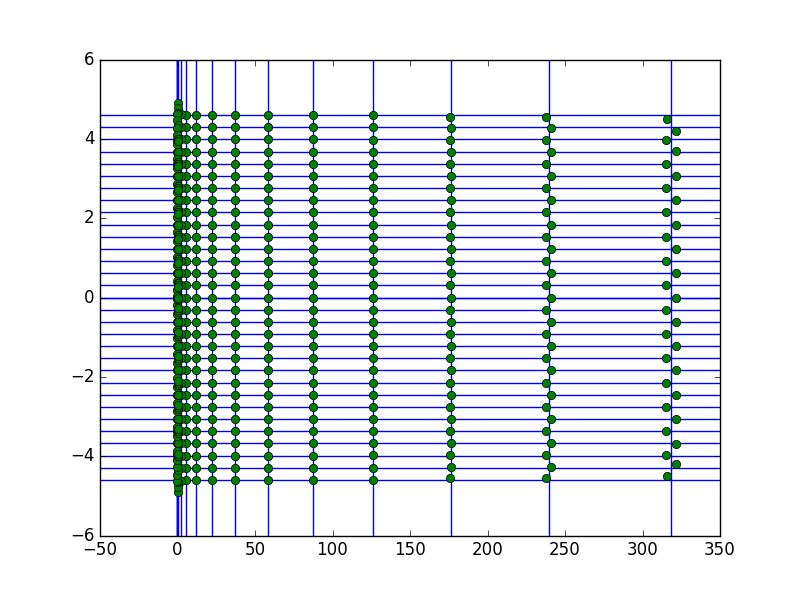
\includegraphics[width=\textwidth,height=.32\textheight]{MNGppo1_spectrum}
\end{minipage}
\\
\begin{minipage}[height=.32\textheight]{.45\textwidth}
\centering \small{\texttt{(b)}}
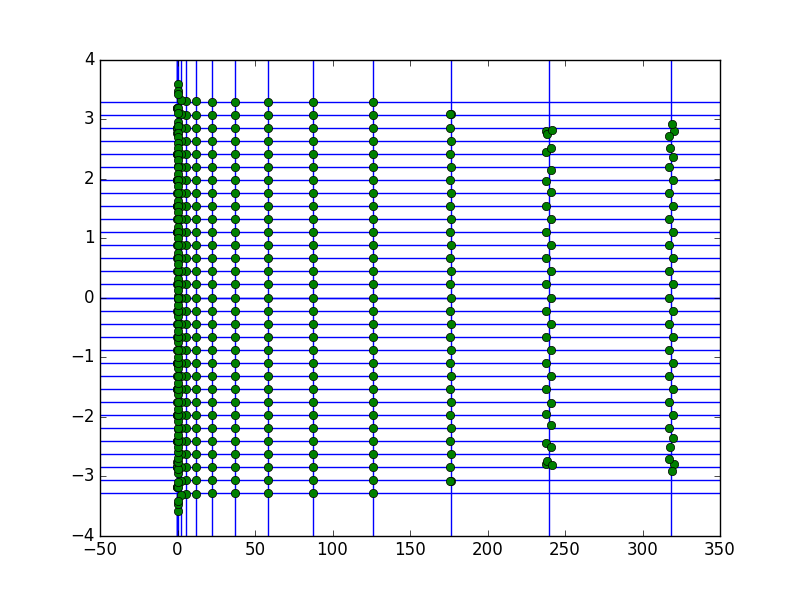
\includegraphics[width=\textwidth,height=.32\textheight]{MNGppo2_spectrum}
\end{minipage}
\begin{minipage}[height=.32\textheight]{.45\textwidth}
\centering \small{\texttt{(c)}}
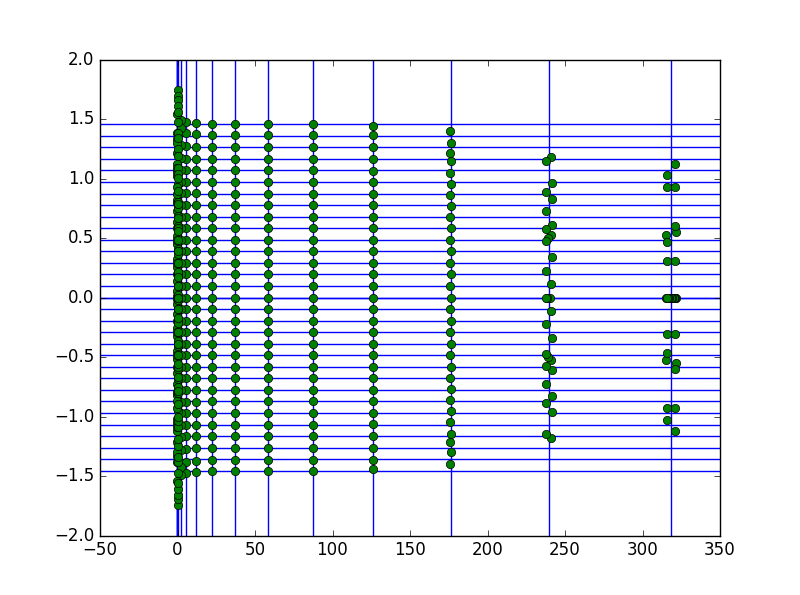
\includegraphics[width=\textwidth,height=.32\textheight]{MNGppo3_spectrum}
\end{minipage}
\caption{ \label{fig:MNGppospacetimespec}
(a) Spatiotemporal multiplier spectrum for \PPO{10.2},
(b) Spatiotemporal multiplier spectrum for \PPO{14.3},
(c) Spatiotemporal multiplier spectrum for \PPO{32.3}.
Intersections between horizontal and vertical lines indicate where the
multipliers would be for the $u(\conf,\zeit)=0$.
In other words, changes from this grid indicate
differences between the linearized spatiotemporal spectrum and the full
spatiotemporal spectrum. All three solutions converged to within machine
precision when defined on a 32-by-32 spacetime grid; Fourier calculations
done with $15 \times 31$ spatiotemporal Fourier coefficients.
}
\end{figure}

In reference to the post of {\bf 2017-03-14},
%\phantomsection\label{2017-03-14MNG} % refer to it by
on page~\pageref{2017-03-14MNG}
in \refchap{chap:dailyBlog}~{\em
Space-time, blogged} I would argue that what I have done is quite similar to
L{\'o}pez \etal\rf{lop05rel}.

By using the spacetime Fourier-Fourier basis representation of the spatiotemporal field with
Galerkin truncations in space and time
\beq   \label{eqn:mng_am_ansatz_ks}
    \am{m}(t)  =  \sum_{n \in \integers} \akj \e^{\ii \omegaj t} \, ,
\eeq
The nonlinear algebraic equations in this basis are \refeq{e-FksSpattemp}.
I will restate the equations here
for completeness and comparison to L{\'o}pez \etal\rf{lop05rel}.
In the spacetime Fourier-Fourier basis, the \KSe\ takes
the form,
\beq
\left[ \ii \omegaj - ( \wavek^2 - \wavek^4 ) \right] \akj
+ \frac{ \ii \wavek }{2} \!\sum_{k'} \sum_{j'}\!\!
\akj a_{k-k',j-j'}
    = 0
\,.
\ee{FkSpattemp}
while in L{\'o}pez \etal\rf{lop05rel}, with the ansatz for {\rpo}
solutions \refeq{eqn:am_ansatz} the \cGL\ take the form
\bea
\ii \left( \frac{2 \pi n}{T} - \frac{\varphi}{T} - m \frac{S}{T} \right)\,\akj
    &=&
    R \akj  - m^2 (1+\ii \nu)\akj
    \label{eqn:spacetime_lop05rel}\\
    - (1+ \ii \mu)\sum_{m'}
      \sum_{n'} a_{k_1,j_1} a_{k_2,j_2} a_{k_3,j_3}^{*}
\,,
\nnu
\eea
where $m_1+m_2-m_3 = m'$ and $n_1+n_2-n_3 = n'$.

The differences between our methods arise when setting up the equation as a root
solving procedure. In L{\'o}pez \etal\rf{lop05rel} the numerics is handled by solving for the
roots of the function $F(\akj ,\varphi , S, T) = 0$ where $F$ is the function described
by \refeq{eqn:spacetime_lop05rel} if one moved all of the terms to one side of the equation.

In my current procedure, I solve
\refeq{e-FksSpattemp}, % PC: Matt had here {eqn:FksSpattemp}
or for comparison,
$F(\akj, T, L) = 0$, where $T,L$ are in the factors $\omegaj,\wavek$ respectively.

I do not explicitly include variables that control the spatial translations of the system and,
up until now, have elected to search for {\rpo} solutions pertaining to
\refeq{e-FksSpattemp} % PC: Matt had here {eqn:FksSpattemp}
by finding them in the first Fourier mode slice. Part of the reason of this was I didn't
understand the reasoning behind parameterizing the spatial translations by $\zeit$ by means
of the factor in the ansatz $\e^{-\ii \wavek \frac{S}{T}t}$. I thought the shift factor
had to be explicitly calculated by the coordinates, and not assumed through this type of time
dependence.

My comments of
{\bf 2017-11-02} on page~\pageref{2017-11-02MNG}
were mainly predicated by the fact that once we find these roots, I don't think
we can apply the same type of reasoning as Politi and Torcini\rf{PolTor92b} as
they aren't truly fixed points of a fictitious dynamical system, like so,
$F(\akj, T, L) = {\akj, T, L}$. But rather, like I have already
described, they are the roots of a system of nonlinear algebraic equations,
$F(\akj, T, L) = 0$.

If I am so inclined to change how I search for relative periodic orbits in the same manner as
L{\'o}pez \etal\rf{lop05rel} I believe all I would have to actually implement is this $\e^{-\ii \wavek \frac{S}{T}t}$
factor in my ansatz, such that the new equations for solutions with $\SOn{2}$ symmetry would be,
\beq
\left[ \ii \omegaj - m \frac{S}{T} - ( \wavek^2 - \wavek^4 ) \right] \akj
+ \frac{ \ii \wavek }{2} \!\sum_{n'} \sum_{m'}\!\!
\akj a_{k-k',j-j'}
    = 0
\,.
\label{eqn:FksSpattemp_rel}
\eeq
such that the spatiotemporal solutions would now be roots of the nonlinear system of equations,
$F(\akj, S, T, L) = 0$

Working my way towards an implementation of the reposed spatiotemporal problem that
involves inverting a differential operator (the sum of second and fourth spatial derivative operators)
defined by equation \refeq{eqn:MNGspacetime_reform}, restated here for completeness.

\bea
G(\Fu, T, L) &\equiv& D_X^{-1}(D_t \Fu + D_x F (F^{-1} \Fu)^2 ) - \Fu = 0
    \continue
D_X &\equiv& D_{xx} - D_{xxxx}
\eea

When treated as the true fixed point problem, the action of $G(x)$ on doubly periodic solutions
is an involution, meaning that points get mapped to themselves. Although this last statement
is obvious, I am stating it because it demonstrates the (what I consider to be)
unnatural behavior of the alternative
problem, where, no matter where you are in this spatiotemporal {\statesp}, every doubly
periodic solution gets mapped to zero under the action of $F$. I believe this to be unnatural
because if you're looking at the linearization of this spatiotemporal function $F$ you are
looking at the linear neighborhood at a point in spatiotemporal {\statesp} that is necessarily
far away from the original doubly periodic solution. Also, the other part I find unnatural about
this is that because every doubly periodic solution is being mapped to zero, all of the solutions
are in a sense being identified to one another no matter where they really exist. There is probably
a smarter and or more precise way of rephrasing that last sentence but its the best I could come up with.

On the other hand, this is also well motivated in a numerical sense because the reformulation
inverts an operator who is comprised of numbers ranging from order unity to numbers orders of magnitude
larger. This is poor for iterative methods unless one introduces a preconditioning, because these large
diagonal elements will a large range of eigenvalues. The reason this is poor, for say, Newton-Krylov method
is that for an example when there is one dominant eigenvalue, the power iteration that produces
the Krylov subspace, $\mathcal{K}_n = {b, Ab, A^2 b, \dots}$ will tend to converge to the most dominant
eigenvector, and hence its known that such methods work best when the eigenvalues are clustered near unity.

So effectively, by reposing the problem by inverting the diagonal operator I am effectively rescaling
space as one might do by either preconditioning or by defining a Sobolev norm to use instead of the
usual $L_2$ norm.

I added code that works in physical space after computing derivatives in Fourier-Fourier space,
the main incentive was to try and see if Jianke Yang's claim that it's better to work in the
"PDE framework" agrees with me. Sadly it doesn't seem to be the case for me. I didn't do things
exactly like he did, and I guess what I in fact implemented could be described by saying
"everything is the same except the linear system of equations that I need to solve are in terms of
the physical velocity field $u$ and not its spatiotemporal Fourier components."

During this process I find it rather confusing and intriguing that the code I have written that
compute hooksteps minimizing the quadratic residual $|A dx - b |^2$ with the constraint $|dx|^2 \leq \delta^2$
where delta is some trust region \emph{seems to only work in physical space for me}. The main culprit is that
when trying to minimize the quadratic form $|A dx - b |^2$ we rewrite this to exploit the fact that
GMRES calculations have already been performed; Namely using the arnoldi iteration recursion relation between
the matrices

\beq \nonumber
A Q_n = Q_{n+1} H_n \, \mbox{where} \,
\eeq

$Q_k$ refers to a matrix whose columns span the $k$th Krylov subspace,

to rewrite the quadratic residual as,
\beq \nonumber
|H_n s - b|^2 \, \mbox{where} \,,
\eeq
$dx = Q_n s$. Performing a singular value decomposition on $H_n$ allows us to simplify the problem such that
linear system becomes diagonal. i.e. with $H_n = U D \transp{V}$, and performing some algebra, we are left with
\beq \nonumber
|D \hat{s} - \hat{b}|^2
\eeq

In the above equation $\hat{s} = \transp{V} s $ and
$\hat{b} = \transp{U} Q_{n+1}^{\top} b$, with $\hat{s}$ being
constrained to be within a trust region described by delta. $|\hat{s}|^2 \leq
\delta^2$. The main way that this problem is tackled by Dennis and Schnable
\rf{Dennis96} is to assume the dependence on a new parameter $\mu$ such that
\[
\hat{s}_i = \frac{\hat{b}_i}{d_i + \mu}
\,,
\]
and then use a modified Newton method to find zeros of the function
\[
\Phi (\mu) = |\hat{s}(\mu)|^2 - \delta^2
\,.
\]

The reason why they use a modified Newton (one that seems to be very specific to the problem) is that
due to the form of the presumed dependence on $\mu$ the regular Newton is found to be suboptimal in
the sense that it always undershoots when making correction. The form of the modified Newton to optimize
this $\mu$ is the following

\beq
\Delta \mu = \frac{|\hat{s}(\mu)| \Phi (\mu)}{\delta \prime{\Phi}(\mu)}
\eeq

which can be seen that the modification is in the form of the prefactor $\hat{s} / \delta$
Testing more stringent conditions to hopefully produce better initial conditions for spatiotemporal
code, they're crude bounds such that during the close recurrence searching procedure there is now a maximum
allowed value for the $L_2$ norm, and after a Poincar\'e intersection has been obtained there is now
a trial to compute what the $L_2$ norm would be for the resultant spatiotemporal mapping. This is helping
produce some better initial conditions which will be passed to the hybrid adjoint Newton-Krylov code I have
currently. I'm also trying to be less brash by choosing a value for the initial domain size that is closer
to the $L=22$ domain size, currently I am trying to find \ppo s for a $L=24$ domain size.

Realized that reformulating the {\rpo} spatiotemporal code to encode the \SOn{2} shift with a parameter is a larger
undertaking then I thought, due to all of the different dependencies of the code I have currently; The general
idea is that the shift can be parameterized by time, although I still feel like this is somehow only incorporating
a specific time of translation; In other words I can't shake the feeling that

The general idea is to produce an ansatz for the relation between endpoints (initial point and the
endpoint i.e. point after one prime period) on a {\rpo} in such a fashion (described in terms of
spatial Fourier modes to make the representation of the translation easier),
\beq \label{e-MNG_rpo_st_ansatz}
\Fu_k(0) =e^{i k S t/T_p}\Fu_k(T) \, ,
\eeq
where the spatial drift, shift, etc. is parameterized by time and a shift parameter $S$. The
form of the rescaled spatiotemporal mapping would then take the following form.
\bea \label{e-MNG_rpo_spacetime_reform}
x &=& (\Fu, T, L, S)
    \continue
G(x) &\equiv& D_X^{-1}((D_t + D_S) \Fu + D_x F (F^{-1} \Fu)^2 ) - \Fu
    \continue
D_X &\equiv& D_{xx} - D_{xxxx}
\eea
where $x$ is a vector representing all of the varying quantities $(\Fu , T_p, L, S)$, and $D_S$
is an operator representing the time derivative of the exponential prefactor in \refeq{e-MNG_rpo_st_ansatz}

Tried to trawl {\statesp} for initial conditions for my spatiotemporal code and realized that
it ran really slowly for small step sizes (large number of steps). Figured out how to speed
it up by rewriting some key parts of the close recurrence calculations; realized I was sloppy
when it came with the actual optimization previously. Essentially by unrolling some 'for'-loops
and rewriting some key portions I was able to dramatically speed it up.

Instead of the Poincar\'e constraint in addition to close recurrence calculations, which
are in my mind somewhat redundant because I'm trying to compute approximations I instead
played around with a number of different procedures that only relied on close recurrence
calculations, i.e. minimizing the $L_2$ norm of the difference between two {\statesp} points.

Something that I experimented with numerically was a procedure that computed a coarse time-integration
and then if the $L_2$ norm was within a certain tolerance, it would be recomputed with an increased number
of time steps. This would produce great initial conditions in a small number of cases, where the local minima in the
close recurrence diagram actually corresponded to a recurrence, as it would rightly increase the accuracy of both
the starting point of the orbit, the ending point, and the period. I'm sort of deciding between this
and just running one close recurrence trawl with fine integration, because in the majority of cases the
local minima of the $L_2$ norm is just happenstance and not related to a useful recurrence. One of the
symptoms of this is that in certain instances the finer time-integration would actually increase
the minimum of the $L_2$ norm. This didn't make sense to me, and could be due to the exact way I had the
procedure implemented, i.e. taking the minimum from the coarse close recurrence procedure and then
using it as the starting point for the fine close recurrence procedure might be too hopeful, and it might
be best to just start at the same point with the same time range.

The way that this was accomplished was by tuning the restart procedure as
well as tuning time integration in the close recurrence procedure, as
well as the total time being integrated, number of time steps. I have
abandoned the Poincar\'e hyperplane in favor of this fine time
integration. I also abandoned playing around with running a coarse time
integration and then refining it as this produced strange results. I
thought that it would merely produce a larger region around the local
minimum (region of the close recurrence plot) by tuning the amount of
time integrated of the second time integration as well as increasing the
number of time steps but sometimes this procedure would either restart in
the wrong spot or miss the local minimum returning a larger (in terms of
the residual of the $L_2$ norm of the difference between starting and
final points.) Therefore, I decided it was wrothwhile due to other
speed-ups to just perform the finer close recurrence and if nothing is
found then just restart.

In between testing these new initial conditions I have decided to rewrite
and add some different ways that the hookstep is calculated. This is due
to there being a lack of safety nets for when the hookstep code
previously would fail and the code would have to abort. This seems to be
due to trying to optimize a hookstep for too large of a trust region.
While normally you would just check the residual and then if it isn't
reduced, one would reduce the trust region and continue. But, in my case
this would lead to numerical overflow and the code would abort.
Therefore, a safer, more constrained optimization protocol had to be
adopted. Now, the parameter that computes the size of the corrections is
always bounded and if it fails to lie in these bounds, a value is chosen
based on the iteration.

In other words when asked to find a vector $\hat{s}$ that minimizes $||D
\hat{s} - \hat{b} ||_2 $ subject to $\hat{s} \leq \delta $, the general
solution is given by\rf{Dennis96,ChanKers13},
\beq \label{eqn:hookstep}
\hat{s} = \frac{\hat{b} d_i}{d_i^2 + \mu} \mbox{    (no summation)}
\,,
\eeq
\ie, this is the solution that minimizes $\Phi(\mu) = ||s(\mu)||^2 - \delta^2$.

Now I will elect to follow the procedure in \refref{Dennis96} that instills bounds on the parameter $\mu$.
The lower bound will be chosen by the ``normal"
Newton procedure instead of the one that is adapted to solve for $\mu$ for this problem.

During each iteration to update $\mu$, we calculate lower($\ell$) and upper (u) bounds by

Initializing them at first by $\ell_0 =- \frac{\Phi(0)}{\Phi^{\prime}(0)}$ and $u_0= |\nabla F(x_c)|/\delta_c$.

Then at each step for the lower bound we increase the lower bound by taking the maximum between

\beq
\ell_{+}^N = \mu_c - \frac{\Phi(\mu_c)}{\Phi^{\prime}(\mu_c)}
\eeq

and the current lower bound.

To update the upper bound we decrease it by taking the minimum between the current upper bound and the
current value of mu,
\beq
u_{+} = min(u_c , \mu_c)
\eeq

where $+$ indicates the next value of the parameters, and ``c" indicates the current value (following
\rf{Dennis96} notation as to not confuse myself).

The next iterate $\mu_{+}$ is calculated by the 'adapted' Newton method.

\beq
\mu_{+} = \mu_c - \frac{s(\mu_c)}{\delta_c} \frac{\Phi(\mu_c)}{\Phi^{\prime}(\mu_c)}
\eeq

and then tested to see if it lies in our trusted region $[\ell_{+}, u_{+}]$. If it doesn't,
then the next iterate $\mu_{+}$ is taken to be $\max ((\ell_{+} u_{+})^{1/2}, 10^{-3} u_{+})$
which Dennis and Schnable claim is most often used to calculate the initial value $\mu_0$.

We then let the iteration run until the norm of the hookstep lies in our trust region. (I might change
this to be until the residual of the function $\Phi (\mu)$ is minimized sufficiently).

After these changes, we then need to decide to do with the trust region and our current hookstep.
If the hookstep does not minimize the residual sufficiently when compared to the linear model,
we need to decrease the trust region radius (which they say they just do by halving it but also give
details on calculating a multiplier between one tenth and one half). If the residual compares
favorably to the quadratic residual then we can keep this as a backup step before increasing the
trust region radius by a factor of two and attempting to try again.

Almost done with the automation procedure to find spatiotemporal fixed points associated
with \ppo s. I combined the initial condition generation code and the solution converging code
into one Python script. What it will do is work through
different domain sizes one-by-one, produce initial conditions for the convergence code, and if
the initial conditions satisfy certain requirements on the residual of the cost functional, run
the convergence code on it. Currently have it setup so that long trawls of {\statesp} are performed
as opposed to shorter more accurate trawls, getting some weird results so it could be the step size
is too large, however.

Fixed the bugs regarding trust region being too large; in which case the optimization procedure
would fail or give nonsensical results because the parameter involved would diverge towards negative
infinity. In other words, it seems to work when the approximate solution first evaluted
at $\mu = 0$ in \refeq{eqn:hookstep} is larger than the trust region. I.e. it works when
$|\hat{s}(\mu = 0)| > \delta$. Then, by the effect of increasing $\mu$ ensures that the solution's norm
is being scaled back to within the trust region. If the norm of $s(\mu = 0) < \delta$ then the optimization
tries to enlarge the approximate solution by making the denominator smaller via cancellation. I find no
mention of the in \refref{Dennis96} but they do have a chapter on rescaling. The reason why this is so confusing
to me is that I thought by using my reformulated, rescaled equations I would have already dealt with any scaling
issues but it seems it isn't so easy. I'm going to test if whether the original formulation shares this property
or not, meaning that it could be the case that the original equations are more useful in using the hookstep
method and the rescaled equations are better for descent and regular Newton methods. I find this hard to be
the case because I know a properly scaled matrix is almost required for GMRES to be useful, as it includes
power iteration of matrix vector products so maybe there is still yet another problem with the hookstep code
that hasn't been found as of yet.

I might elect to do a different residual criterion that just uses norms, right now it calculates
a time integration series, and its reflection. Then the close recurrence criterion is based on the
$L_2$ norm between the reflected series and the physical one; the rational being that if we pass
through one prime period of a \ppo, then the endpoint should be the reflected partner
of the initial point. The problem with this is for every time $t$ the $L_2$ norm of the difference
with every reflected future point must be computed. A more efficient solution might be to just compute
all of the $L_2$ norms once and then trust that if an initial point has a similar norm of a reflected
endpoint, then they are symmetric under reflection. This seems hopeful, and I feel like I'm almost
being academically dishonest at this point because this is yet another idea from L{\'o}pez \etal\rf{lop05rel}.

Reformulating the \rpo\ portion of the code to use a co-moving frame. This is the only option I believe
if I would like to rescale the equations, as the first Fourier mode slice would be very nasty. This method
also avoid rescaling time.

The general idea is akin to L{\'o}pez \etal\rf{lop05rel} where the approximate solution or initial condition is shifted
into the co-moving frame to first make the initial condition truly periodic and then the inverse shift
is kept track of so that the ``true" solution (the one in the initial frame) can be recomputed after
convergence. If I've understood everything this should allow for the following equations, note the very
similar rescaling by the inverse of the diagonal operator containing the second and fourth powers of the wavenumber.

The one trade-off of this method is increasing the dimensionality of the problem by one, this is because of the extra
parameter keeping track of the shift.

\bea \label{eqn:rpo_spacetime_reform}
G(\Fu, T, L) &\equiv& D_X^{-1}((D_t + S) \Fu + D_x F (F^{-1} \Fu)^2 ) - \Fu = 0
    \continue
D_X &\equiv& D_{xx} - D_{xxxx}
    \continue
S   &\equiv& diag(\frac{-i m \ell}{T})
\eea

where, the definition of the operator $S$ comes naturally from the definition of the shift required to transform from the
co-moving frame to the initial frame, $\hat{\Fu} = e^{\frac{-i m \ell_p t}{T}}\Fu$.
I'm cheating for the sake of simplicity in typing the equations because
I'm actually using the real-valued representation where the operator is actually an off diagonal \SOn{2} type matrix.

With the concept of a very small number of active spatiotemporal modes, usually due to discrete symmetries
I applied this in a very rough way to test the number of active modes in one of the shortest orbits (in time)
of the HKW computation cell, also known to channelflow users as "p19p02".

I first took $M=16$ points in time (16 snapshots) of the shortest periodic
orbit whose spatial discretization requires $N_x = 32 \times N_y = 49 \times N_z = 32 \times 3 = 150528 \equiv dim(\mathcal{M}_{xyz})$ physical
space variables to describe. The total number of variables in the spatiotemporal discretization is then $150528*16 = 2408448$.

To test the number of "active modes" spatiotemporally, I used real-valued FFTs in the spanwise and streamwise direction, and
the discrete cosine transform (which I think is equivalent to the Chebyshev coordinates but I could be drastically wrong) in the
wall normal direction. To describe the number of active modes I counted the number of spatiotemporal coefficients,
now $(Fourier \times Fourier \times Chebyshev) \times Fourier$ in three directions,
had a absolute value (not the square) that was greater than $10^{-14}$.

I claim that in the shortest periodic orbit 'p19p02' is
$N_{active} = 564477$. In other words, approximately seventy-five percent of the spatiotemporal information is redundant/not used.
Therefore, for a full spatiotemporal description using 16 points in time in this basis, the number of variables used
to describe it only increases by a factor of $3.74998007015$. This is a nontrivial increase in dimensionality,
but much less than the expected multiple of $16$.

For $M=32$ the reduction percentage increases, but so do the number of modes corresponding to time. The multiple for
$M=32$ was $7.26536591199$,  which is slightly less than two times the $M=16$ multiple. I believe that this is due
to extra modes in time which themselves are non-active.

I still need to test this on a case that has non-zero shift, but in order to exploit these methods I need a truly periodic
orbit not a fundamental domain, so the number of points in time would have to increase by two, and I am unclear whether
it would be as beneficial or even better.
I'm indebted to Roman because even though I've scoured the literature for a
matrix free representation of the product $\transp{J} x$, he pointed out that
Ravi did this, and after some thought I realized that if I can explicitly
form the \jacobianM, then reverse engineering what this matrix vector product
might be possible. The problem lies in the fact that Ravi used finite
differences to define derivatives so that the product with the transpose is
much more straightforward.

In my Fourier-Fourier description this is going to be harder, but I believe
that the only difficulty will be the reverse engineering of how to compute
the nonlinear component, as the linear component is fairly straightforward.

In more depth, the action of the linear component for $\Zn{2}$ type solutions
can be represented by matrix multiplication by a tridiagonal matrix, with the
main diagonal being filled with $-q_n^2 +q_n^4$, and the two off diagonals
filled with terms $\pm \omega_m$ (no $\ii$ because in real-valued
representation). Therefore action of the transpose only affects these off
diagonal terms by swapping the signs of them $\pm \omega_m \rightarrow \mp
\omega_m$. This is exactly the action produced by sending $T \rightarrow -T$.

Therefore, the linear component of the matrix vector product (here $lin$
subscript denotes `linear'),
\beq
J_{lin}^{\top} (\epsilon dx)
= \frac{1}{\epsilon}
(F_{lin}(u+\epsilon du,-T+ \epsilon dT,L+ \epsilon dL) - F_{lin}(u,-T,L))
\,,
\ee{eqn:linear_action_transpose}
where $dx = \{du,dT,dL\}$.
Because the transposition only affects the component of the \jacobianM\ that is
constituted by swapping the sign of the time derivative, we can make the
substitution in the function call.

The main goal is to be able to write the matrix-vector product in terms of
function calls so that no matrices are explicitly formed. This would
dramatically increase the speed at which my adjoint descent code runs and due
to the global convergence of the method, and the speed when used in a hybrid
method, this might be exactly the robustness that we need to find large
doubly-periodic spacetime solutions at least.

More work into \rpo\ matrix-vector product formulation of the spatiotemp code.
Still trying to figure out what I can use as extra constraints.
For \ppo s I can still constrain to be transverse to time translations
to give me corrections but because of the reflection symmetry I cannot
impose tranversality to the spatial translation direction, which is what
is used to complete the underdetermined linear system. Maybe I'm thinking
about it the wrong way as usually these are just implemented as constraints
to prevent the Newton correction from pointing in symmetry directions,
and so I might be able to use the

I sort of went down a rabbit hole as to test what extra constraints are possible
I tested a constraint the prevents changes in area. This was easy enough
to implement, and it worked, but its the exact opposite of what I would
like to accomplish. The tangent space(s) are what should be telling me
the correct scales for $L$ and $T$. Because of this I tried to impose
a constraint such that the area is minimized but I can't currently
think of a way that doesn't do this \emph{too well}. What I mean by
this is that if you say that you want to minimize $T*L$ then it will
just send one of those parameters to $0$, naturally.

One interesting thing that came about from the area constraint is
that if you tell my code the wrong area. If for instance I changed
$L_0$ to $L_0 - 2 = 20$ then it had to change the characteristic
wavelength in time to fit in my box. Including figures for scientific
curiousity.

The main idea I'm trying to flush out here is that if I cannot use
tranversality constraints to complete the linear system then
perhaps I need to complete the linear system by creating constraints
on the parameters themselves.

Investigated this method in hopes that maybe I could prove Burak wrong
by including "pseudo arc-length continuation" in the actual spatiotemporal
code at the same, but sadly it doesn't look like one can have cake and eat
it too.

Wrote the ``reformulated" (rescaled) version of the mean velocity frame
code for \rpo\ {\twots}. As expected, it works a lot better
with iterative methods such as GMRES.

I'm only able to get away with this reformulation because the diagonal
terms corresponding to laplacian and laplacian squared operators
dominate. For the mean velocity frame representation of
\RPOtwot{22}{16.3}, %\RPO{16.3}
the condition number is reduced to around $\kappa \approx 2000$ which is
about an order of magnitude better than \ppo\ {\twots}.

It seems that these reformulations will be necessary as the matrix free
code relies on approximations to iterative methods. When the iterative
methods fail for the exact problem (explicitly formed matrices) I know
I'm in danger. Luckily the test cases I've run through where, for
instance, GMRES fails for the original equation but succeeds with the
reformulated equations. Like I have mentioned before the reformulation is
sort of a cheap trick I am using that could essentially be accomplished
by preconditioning but I came up with some kooky ideas I want to try out
to see if the reformulation of {\twots} actually induces
an iterative map or if I just think it does. Maybe I'm in fantasy land
but because I am essentially rewriting \refeq{e-FksSpattemp},
%Predrag 2018-03-21 was \refeq{eqn:FkSpattemp} ??
which can
be drastically simplified as $F(u,T,L,\sigma) = 0$, as another equation
$\tilde{F}-\Fu = 0$. I think the physical interpretation of the second
equation is much clearer than the first, but it has its own issues as it
demands for inversion of an operator that can technically become
singular. The reformulated equations for the mean velocity frame

This was not the equation I put in practice as the inversion of
the Laplacian and Laplacian squared term turned out to not be useful.}
        }
\beq \label{eqn:MNGspacetime_reform_mvf}
G(\Fu) = (D_{\conf \conf} - D_{\conf \conf \conf \conf})^{-1}
    ((D_{\zeit}+S) \Fu + D_{\conf}F((F^{-1} \Fu)^2)) -\Fu = 0,
\eeq
where $S$ is the derivative of the Lie algebra element,
$\dot{\phi}\cdot \mathbb{T}=  {2 \pi n \sigma}/{TL}$,
such that ${2\pi \sigma}/{L} =\theta$ is the parameter needed to perform
\SOn{2} group action.
\beq \label{eqn:MNGspacetime_mvf}
G(\Fu) = (D_{\zeit} + S + D_{\conf \conf} - D_{\conf \conf \conf \conf}) \Fu
          + D_{\conf}F((F^{-1} \Fu)^2)) = 0,
\eeq
where $S$ is the derivative of the Lie algebra element, $\dot{\phi}\cdot
\mathbb{T}=  {2 \pi n \sigma}/{TL}$, such that ${2\pi \sigma}/{L}
=\theta$ is the parameter needed to perform \SOn{2} group action.

Now that I am comfortable with saying the direct-matrix (forming matrices explicitly)
methods will work for both $\Zn{2}$ and \SOn{2} isotropy subgroup (\rpo\ in its mean velocity frame)
solutions I have been working on the matrix-free methods. This was done in a poor order
however because I should have made the changes to the automated {\twot}
finder to run on light while figuring this out.

I believe the main source of error (due to the fact that I am using the same exact gmres code)
for certain test cases is that the matrix-vector approximation is just too inaccurate to
produce a reliable Krylov subspace to find solutions in. I'm attempting to work around this with
higher order finite difference approximations for the matrix-vector approximations, but the difference
upon the first iteration between the first order ($\mathcal{O}(\Delta x)^2$ error) and the higher
order ($\mathcal{O}(\Delta x)^4$ error) is approximately $10^-10$. I need to compare the finite difference
approximation to the explicit matrix computation still.

Realized that perhaps adjoint descent would be better applied to full {\statesp} as opposed to spatiotemporal
symmetry subspaces because its an integration(descent) type method. I wrote new codes that apply adjoint
descent to the complex representation of the spatiotemporal \KSe, \ie\
\refeq{e-FksSpattemp}. % PC: Matt had here {eqn:FksSpattemp}
The main benefit of doing so is that in the real-valued representation that I
use for everything it isn't straight forward how to calculate the transpose of
the Fourier transform and inverse transform operations, but when I use a
complex representation the transformation is unitary; meaning that the
conjugate transposes that arise are easily replaced using the unitarity
property of the Fourier transform (with proper normalization).

Currently running tests on spatiotemporal domains initiated from random noise, large scale domains, and seeing
what comes out. Random noise on a $T,L = 500,500$ domain ran long enough starts to pick out the length scales of
the \KSe, and its the matrix-free computation that allows it to run fast enough to do anything.

\refFig{fig:MNGlarge_adjointdescent} is an example of the limits of the method so far. Taking (pseudo) white
noise on a large space-time domain and then running the adjoint descent reproduces structures that look similar to those
seen within simulations of the \KSe.

Another topic I need to breach is whether I can constrain the adjoint descent to
 preserve the symmetry subgroup of any solutions found. If I can get the matrix-free
  method to work in the real representations this will automatically hold but not
   so in the complex representation as I'm abusing the extra variables and unitarity
    of the Fourier transform so that everything is unconstrained.

\begin{figure}[ht]
\begin{minipage}[height=.32\textheight]{.45\textwidth}
\centering \small{\texttt{(a)}}
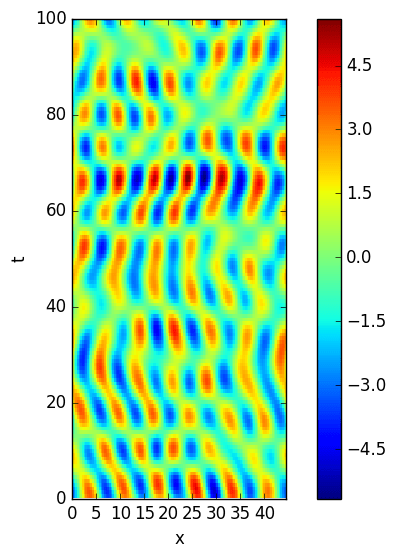
\includegraphics[width=\textwidth,height=.32\textheight]{MNG_T100L44_init}
\end{minipage}
\begin{minipage}[height=.32\textheight]{.45\textwidth}
\centering \small{\texttt{(b)}}
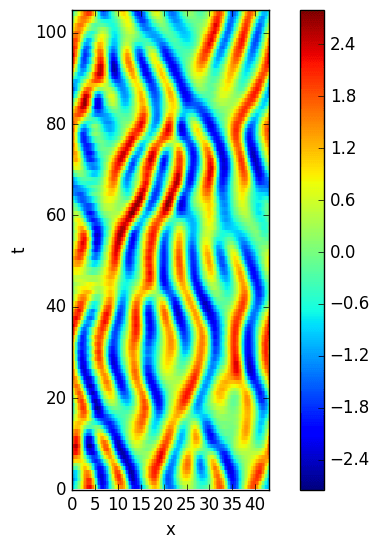
\includegraphics[width=\textwidth,height=.32\textheight]{MNG_T100L44_final}
\end{minipage}
\caption{ \label{fig:MNG_spacetime_smoothed}
(a) Smoothed and $\bar{L}=2\pi\sqrt{2}$ modulated ``noise''
initialized on a spacetime domain
$(L_0,T_0)=(5\bar{L},100)=(44.4,100)$. Initial residual $F^2 = 1808$.
(b) Resultant \twot\ after meeting tolerance
$F(\tau)^2= 1.86<10^{-3} F(0)^2$.
$(L_f,T_f)=(43.066,105.08) = (L_0 - 1.363,T_0 + 5.08)$.
The computation took only 7 CPU seconds on my laptop.
}
\end{figure}

\begin{figure}
\begin{minipage}[height=.32\textheight]{.45\textwidth}
\centering \small{\texttt{(a)}}
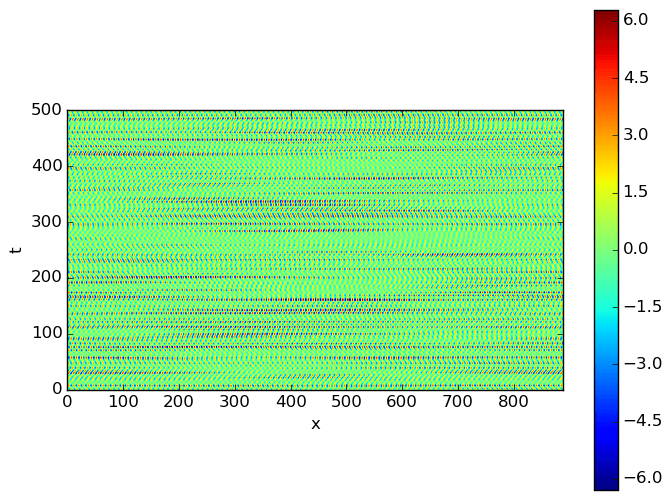
\includegraphics[width=\textwidth,height=.32\textheight]{MNG_T500L888_init}
\end{minipage}
\\
\begin{minipage}[height=.32\textheight]{.45\textwidth}
\centering \small{\texttt{(b)}}
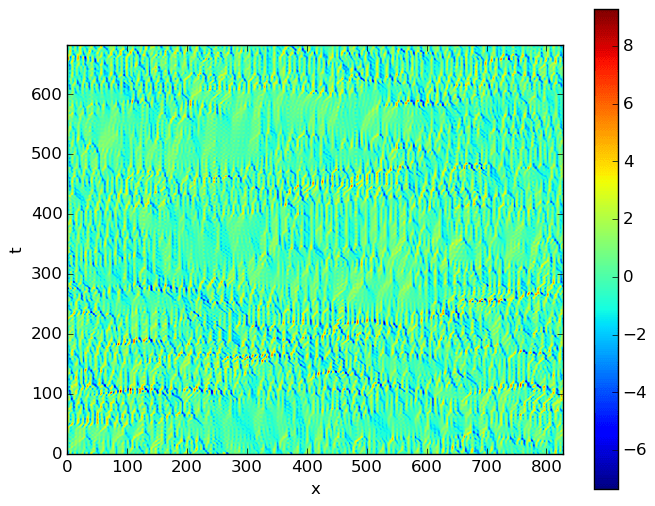
\includegraphics[width=\textwidth,height=.32\textheight]{MNG_T500L888_final}
\end{minipage}
\begin{minipage}[height=.32\textheight]{.45\textwidth}
\centering \small{\texttt{(c)}}
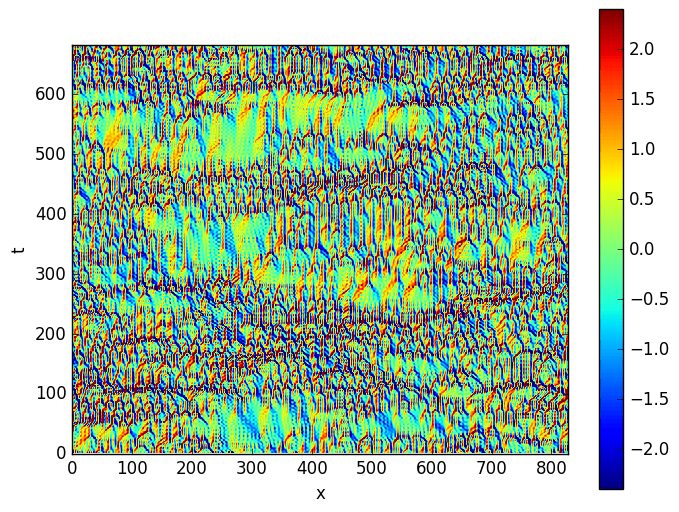
\includegraphics[width=\textwidth,height=.32\textheight]{MNG_T500L888_capped}
\end{minipage}
\caption{ \label{fig:MNG_spacetime_capped}
(a) Smoothed noise initialized on a spacetime domain $T=500$,
$L=100\,\bar{L} \approx 889$, where $\bar{L}=2\pi\sqrt{2}$.
Initial residual $F^2 = 16635$
(b) Resultant spatiotemporal field after one-hundred thousand adjoint descent
steps $F^2_f = 3.66$, $T_f = 682.62$, $L_f=828.31$.
(c) The same $u(x,t)$ as in (b), except with the displayed values constrained
between $-2.4 \leq u(x,t) \leq 2.4$. Computation time was approximately an hour
and ten minutes.
}
\end{figure}


While laying in bed for hours I had what I at the time thought was a good idea which begged the question
``If I can add a term to \refeq{eqn:MNGspacetime_reform_mvf} so that it knows its working with solutions
with \SOn{2} symmetry. Why cannot do the same for solutions with \Zn{2} symmetry?"

The general idea is this.
I know how to act the reflection symmetry onto the equations, can I not create
an ansatz or modify the cost functional that mimics the way L{\'o}pez
\etal\rf{lop05rel} deal with rotational symmetry?

The first idea was borne from the fact that the \KSe\ under reflection are still equal to zero
by equivariance,
\beq
-u_{\zeit}(-\conf,\zeit)
-u_{\conf \conf}(-\conf,\zeit)
-u_{\conf \conf}(-\conf,\zeit)
-u(-\conf,\zeit)u_{\conf}(-\conf,\zeit)=0,
\ee{KS_reflected}
So is there not a way to use this to reformulate (yet again) my problem in such
a way that I achieve a complex representation for solutions with \Zn{2}
symmetry?

\PCedit{%2018-04-17
The reflection operator $\Refl$ acts on coordinate $x$ as $\Refl x=-x$, and on
the velocity field $u$ (dimensionally $[x]/[t]$) as $\Refl u(x,t)=-u(-x,t)$.
Relation $\Refl^2 = 1$ induces\rf{DasBuch}
linear decomposition $u(x) = u^+(x)+ u^-(x)$, $u^\pm(x)= P^\pm u(x) \in
\bbU^\pm$, into irreducible subspaces $ \bbU = \bbU^+ \oplus \bbU^-$, where
\beq
    P^+=(1+\Refl)/2
    \,,\qquad
    P^-=(1-\Refl)/2
\,,
\ee{P1P2projMNG}
are the antisymmetric/symmetric projection operators.
Applying $P^+,\,P^-$ on the \KSe\ \refeq{e-ks} we have\rf{KNSks90}
\bea
 u_t^+ &=& - (u^+u^+_x + u^-u^-_x )
                - u^+_{xx} - u^+_{xxxx}
    \continue
 u_t^- &=& - (u^+u^-_x + u^-u^+_x )
                - u^-_{xx} - u^-_{xxxx}
\,. \label{KSD1MNG} \eea If $u^- = 0$, \KS\ flow is confined to the
antisymmetric $\bbU^+$ subspace, \beq
 u_t^+ = - u^+u^+_x
                - u^+_{xx} - u^+_{xxxx}
\,,
\label{KSU+MNG}
\eeq but otherwise the nonlinear terms in \refeq{KSD1MNG}
mix the two subspaces.
}

Let's first write \refeq{KS_reflected} in a more suggestive form:
\beq
\exp{\ii \pi}(F(u(-\conf,\zeit))) = \Refl \circ F(u(-\conf,\zeit))
\eeq

The first idea was okay, well $0+0 = 0$ so let's see what that yields in terms of the cost functional,
let $\Refl$ denote the operation of reflection, then
\beq
\tilde{F} \equiv F + \Refl \circ F,
\eeq
leads to a {\color{red} completely wrong, just elaborating on my though process} cost functional,
\beq
G = \frac{1}{2}\tilde{F}^{\dagger} \tilde{F} =  \frac{1}{2}((1+e^{\ii \pi})F)^{\dagger} ((1+e^{\ii \pi})F) \,
\ee{costfunctionaltestone}
but carrying out this calculation leads to the trivial result $G=0$ due to cancellation. Likewise, a definition
\beq
\tilde{F} \equiv F + \Refl \circ F,
\eeq
just leads to an extra factor of $4$ in the original cost functional equation, but would technically alter the adjoint
direction, explicitly
\bea \label{costfunctionaltesttwo}
G &=& \frac{1}{2}\tilde{F}^{\dagger} \tilde{F} \continue
  &=&  \frac{1}{2}((1-e^{\ii \pi})F)^{\dagger} ((1-e^{\ii \pi})F) \continue
  &=& \frac{1}{2}F^{\dagger} (1-e^{-\ii \pi})(1-e^{\ii \pi})F \continue
  &=& 2 F^{\dagger}F
\eea
therefore there would be no change in the adjoint direction $-J^{\dagger} F$ outside of a scalar
multiple.

I haven't given up hope yet however, as these formulations forgot the implicit flipping $x \rightarrow -x$
that is contained within the scalar field itself $u(-\conf, \zeit)$. I think that we can exploit this.

When not using the fundamental domain, a reflection applied to a \ppo\ produces an equivalent solution but
not an invariant solution. This is because in terms of a spatiotemporal tile, the "top" and "bottom" (fundamental
domains) get switched. Therefore in order to have an invariant representation of the solution, we need to translate
in time by $T_p$. In other words, this is how the reflection operation acts on a \ppo when viewed as a periodic orbit,
and not from the fundamental domain perspective.
\beq
\Refl \circ
\begin{bmatrix}
 -u(-\conf,\zeit) \\
 u(\conf,\zeit)
\end{bmatrix}
=
\begin{bmatrix}
u(\conf,\zeit) \\
-u(-\conf,\zeit)
\end{bmatrix}
\ee{reflection_operation}

As we can see, the "bottom" $0 \leq t \leq T_p$ has been switched with the
"top" $T_p \leq t \leq 2 T_p$, therefore in order to enforce invariance under
\Zn{2} symmetry we also need to impose a time translation.
\beq
T \circ \Refl \circ
\begin{bmatrix}
 -u(-\conf,\zeit) \\
 u(\conf,\zeit)
\end{bmatrix}
=
T \circ
\begin{bmatrix}
u(\conf,\zeit) \\
-u(-\conf,\zeit)
\end{bmatrix}
=
\begin{bmatrix}
 -u(-\conf,\zeit) \\
 u(\conf,\zeit)
\end{bmatrix}
\ee{invariant_reflection_operation}

So what if we compose a function, that enforces this? Will it enable a symmetry
constrained calculation much like the mean velocity frame equation? With
\beq
\tilde{F} = (1 + T \circ \Refl\,\circ)F \,,
\ee{reflection_invariant_F}
the cost functional becomes
\beq
G = \frac{1}{2}\tilde{F}^{\dagger} \tilde{F}
  =  \frac{1}{2}((1 + T \circ \Refl \circ)F)^{\dagger} ((1 + T \circ \Refl \circ)F) \,
\ee{invariant_cost_functional}
which I do not think can be simplified. However, this affects the adjoint
descent in a non-trivial way. It requires $\tilde{F}$ be equal to zero, not
only that $F=0$.

\renewcommand{\Refl}{\ensuremath{\sigma}}



These ideas arose due to the nature of handling how to keep \ppo\ type {\twots} invariant
under symmetry. For a generic solution of the \KSe\ that has not been compactified in time, the general
symmetry group would be $\On{2} \times \mathbb{R}$, as any time translation is valid as the equations
are autonomous. Once we compactify time and assume doubly periodic solutions, then we should compactify
time as well such that the general symmetry group of doubly periodic solutions is $ G \equiv \On{2} \times \SOn{2}$.

When viewed from this context we can identify the isotropy subgroups of $G$ for each type of solution.
These are not symmetry actions which the solutions are equivariant under but rather the symmetry actions
that the solutions are \emph{invariant} under.

\beq
G_{x} = \{g \in G : g x = x \}
\ee{symmetry_invariance}

With this definition, the isotropy groups of the different types of solutions have the following isotropy
groups:
\begin{table}[h!]
\centering
\begin{tabular}{c|c}
\hline
RPO & $\{ e, e \}$ \\
PPO & $\{ e, e \} \cup \{ \sigma, \pi \}$ \\
ANTI & $\{ e, e \} \cup \{\sigma, e \}$ \\
\hline
\end{tabular}
\end{table}
where $\sigma$ represents the reflection operation of $\Zn{2}$ and $\pi$ is
the proper rotation by $\pi$, or equivalently the non-identity element of
$\Cn{2}$. Therefore, for \ppo\, type solutions we \textbf{cannot} write the
isotropy group as $\Zn{2}\times\Cn{2}$ as we need an even smaller subgroup.
For the antisymmetric \po s $\in\bbU^+$ the isotropy group is
$\Zn{2}\times{e}$, and for \rpo\, 's there is only the trivial isotropy
group.

This is sort of backwards in the way that we usually view symmetries of solutions, but I believe its because
we usually list the symmetries that a solution is equivariant under and not invariant under.
The logic behind this is that any infinitesimal transformation
(spatial or time translation) will not leave the solution invariant; therefore,
the only possible isotropy subgroups are discrete subgroups of $\On{2} \times \SOn{2}$.


\begin{figure}
\begin{minipage}[height=.32\textheight]{.5\textwidth}
\centering \small{\texttt{(a)}}
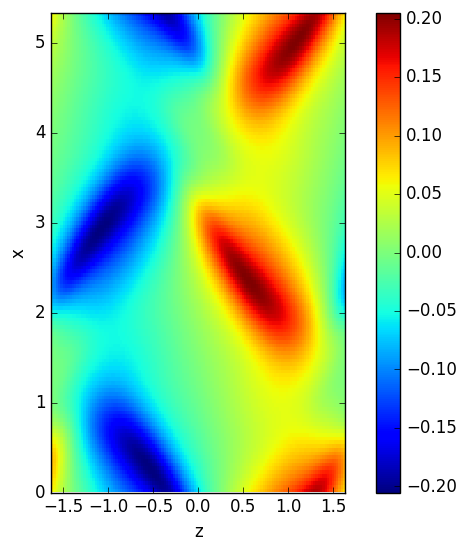
\includegraphics[width=\textwidth,height=.32\textheight]{MNG_nbeq}
\end{minipage}
\begin{minipage}[height=.32\textheight]{.5\textwidth}
\centering \small{\texttt{(b)}}
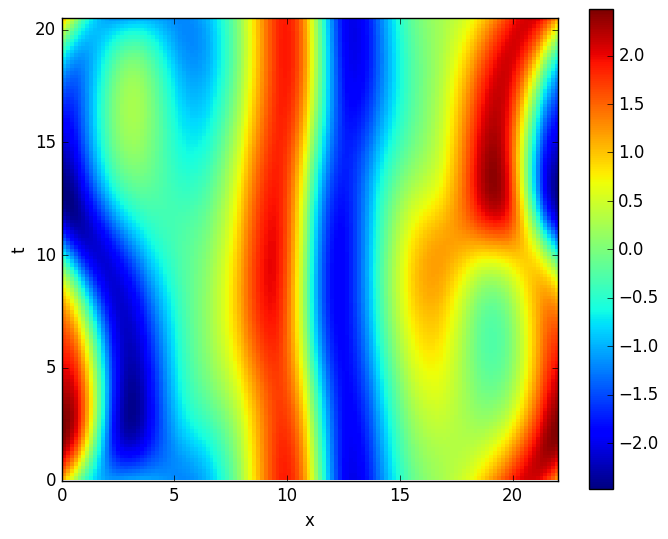
\includegraphics[width=\textwidth,height=.32\textheight]{MNG_ppo1_init}
\end{minipage}
\begin{minipage}[height=.32\textheight]{.5\textwidth}
\centering \small{\texttt{(c)}}
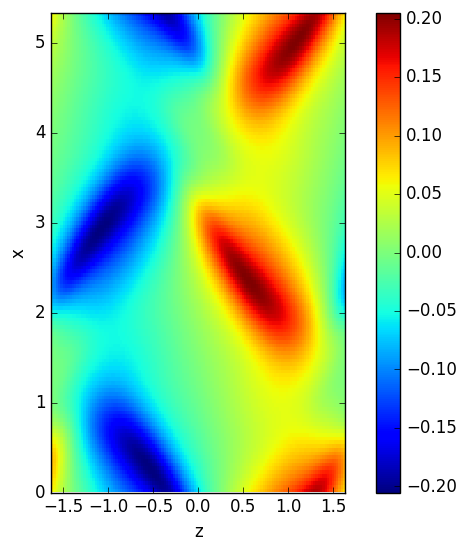
\includegraphics[width=\textwidth,height=.32\textheight]{MNG_nbeq_SR}
\end{minipage}
\begin{minipage}[height=.32\textheight]{.5\textwidth}
\centering \small{\texttt{(d)}}
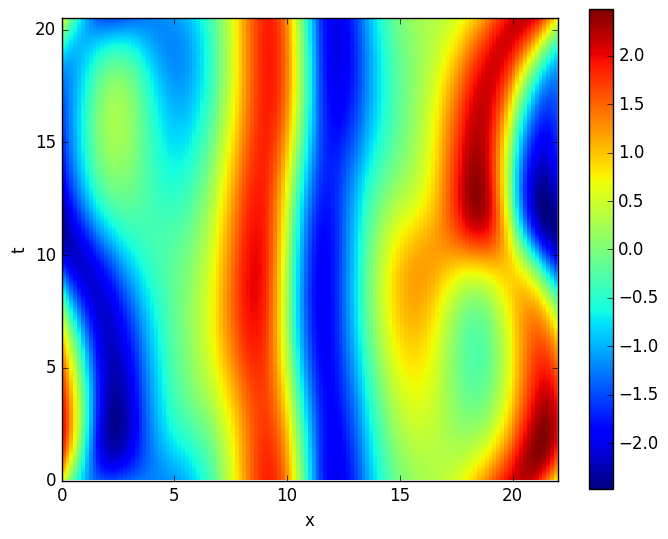
\includegraphics[width=\textwidth,height=.32\textheight]{MNG_ppo1_SR}
\end{minipage}
\caption{ \label{fig:MNG_shiftreflect}
(a) Plot of  the $z$ component of the vector
velocity field $w(z,x)$ at the wall-normal midplane $y=0$, $y \in [-1,1]$
from ``newbie" equilibrium of \pCf.
(b) The shortest preperiodic orbit \KS\ \PPOtwot{22}{10.2}. %, $L=22$ domain size.
(c) Shift and reflected $-w(-z,x+\frac{L_x}{2})$ version of (a).
(d) Shift and reflected $-u(-x,t+\frac{T}{2})$ version of (b).
}
\end{figure}

It turns out that the subgroups are identical and they provide a great chance for
an analogy between \pCf\ and the \KSe. In \reffig{fig:MNG_shiftreflect}
we take the wall normal
midpoint $y=0$ of the newbie equilibrium, and then plot the $z$ component of the
velocity vector, $w(z,x)$ (the order of the variables has a purpose). We also
plot the spatiotemporal scalar field of the shortest preperiodic orbit $u(x,t)$.
Then in (c) we the apply shift-reflect symmetry from the plane Couette,
and in (d) we apply the spatial reflection and time translation symmetry on
the \KS\ solution.
Because both solutions are invariant under these symmetries (c) and (d) are
exact copies of (a) and (b) respectively, but if we compare the equations for the
symmmetry transformation we can see the analogy take shape.

\bea \label{shiftreflect_comparison}
s_1 w(z,x) &=& -w(-z,x+\frac{L_x}{2}) \continue
\sigma \tau u(x,t) &=& = -u(-x, t+\frac{T}{2})
\eea

Therefore, the two dimensional spatial cross section $(z,x)$ of the $z$ component
of the velocity field of \pCf\ has the same symmetry as the
two dimensional \emph{space-time} preperiodic orbit of the \KSe.

The implication of this is that there is now a very precise definition of what
we mean by preperiodic orbit. It is a {\twot} that satisfies
shift(in time) and reflect(in space) symmetry equivalent to two spatial
dimensional plane Couette cross-section.

Therefore not only do we believe all of the machinery available to us from \refrefs{SCD07,GHCW07}
is applicable to spatiotemporal discrete symmetry subgroups in the \KSe, but also we believe
this fact to be a bridge to the gap between spatiotemporal \KSe\ and \pCf.

The next topic of discussion was about how to approximate the time scale for large
{\twots}, as the spatial scale is already pretty well understood as
being the most unstable wavelength of the \KSe. We've been using an approximation
of the temporal scale of about ten to twenty dimensionless time units but we discussed
and thought of a number of ways we can approximate the time scale.

\begin{itemize}
\item Count and average the number of maxima and minima in time strips of the scalar
    field originating from a large {\twots} to give an average wavelength
\item Count the number of maxima and minima in space, and see if and when this number changes.
    Numerically, this would be tracking when the spatial waveform has a "birth or death" event.
\item Combine or compare the previous two methods to see if \PCedit{if what?}
\item Use the "slope" of traveling wave solutions, exponents of $EQ_2$ (dynamically relevant)
    \eqv.
\item Use Lyapunov time


Figured out how shift and reflect subspace for complex Fourier representation (\ppo\ subspace).
It's much easier than I previously thought and was doing this morning, which was taking the real-valued
expression and substituting complex exponentials for sines and cosines.
First the complex spatiotemporal Fourier transform, $m$ is the spatial index, $n$ is the time index

\beq
u(\conf,\zeit) = \sum_{m=-M/2,n=-N/2}^{m=N/2-1,n=N/2-1} \Fu_{nm}e^{\ii(q_m \conf + \omegaj \zeit)},
\eeq

which we then perform shift and reflect symmetry operation on,

\beq
\tau \Refl u(\conf,\zeit) = \sum_{m=-M/2,n=-N/2}^{m=N/2-1,n=N/2-1} -\Fu_{nm}e^{\ii(q_m (-\conf) + \omegaj (\zeit+\frac{T}{2}))},
\eeq

which after some simplification can be written,

\beq
\sum_{m=-M/2,n=-N/2}^{m=N/2-1,n=N/2-1} (-1)^{n+1} \Fu_{nm}e^{\ii(q_m (-\conf) + \omegaj \zeit)}
\eeq

We can't equate them just yet, but I found it most useful to make the transformation $m\rightarrow -m$ in
the original sum rather than the sum after the symmetry operation, this transformation yields the following
equation,

\beq \label{shiftreflect_ppo_complex}
(-1)^{n+1} \Fu_{nm} = \Fu_{n,-m} \,.
\eeq

Now using this, in combination with the two-dimensional conjugacy relation for the two dimensional
Fourier transform of a real valued field $\Fu_{nm} = \Fu_{-n,-m}^{\dagger}$, we can figure out
the invariant subspace, or at least the non redundant set of Fourier coefficients that we need
to reproduce $u(\conf,\zeit)$.

In order to explain this, I will do it pictorially, as the
spatiotemporal Fourier transform is easiest to represent in two
dimensions (i.e. a matrix).

\begin{table}[h!]
\centering
\begin{tabular}{|c|c|c|c|c|}
\hline
\quad  $n\;\setminus\; m$
                  & $0$  & $1,\ldots,M/2-1$                & $-\frac{M}{2}$ & $-M/2+1,\ldots,-1$ \\
\hline
$0$               & $0$  & $\Fu_{0m}$                     & $0$            & $-\Fu_{0,m}$        \\
\hline
$1,\ldots,N/2-1$  & $0$  & $\Fu_{nm}$                     & $0$            & $(-1)^{n+1}\Fu_{nm}$ \\
\hline
$\frac{-N}{2}$    & $0$  & $0$                             & $0$            & $0$                 \\
\hline
$-N/2+1,\ldots,-1$ & $0$  & $(-1)^{n+1}\Fu_{nm}^{\dagger}$ & $0$           & $\Fu_{nm}^{\dagger}$ \\
\hline
\end{tabular}
\end{table}
where the coefficients $\Fu_{nm}$ in this table only imply positive indices, $n>0$ and $m>0$. So in order to
reconstruct the original field $u(\conf,\zeit)$ we only need the spatiotemporal modes consisting of indices $ n \geq 0$
and $m > 0$. The rest of the table is purely instructions on how to recreate the spatiotemporal spectrum so that the
inverse Fourier transform can be applied.

Almost done implementing the new complex valued codes for the shift-reflect
subspace and spatiotemporal \rpo\ codes, or so I thought before the previously
described investigation.

For the shift-reflect complex-valued code it seems that the $L_2$ norm is a much better
measure that it was in any of the previous codes. My favorite test case, \PPOtwot{22}{10.2}
on $L=22$ domain starts with an initial cost function residual of $\frac{1}{2}|F|^2 \approx 10^{-9}$
and is able to converge to within machine precision using adjoint descent alone in under one second.
This result uses a 32-by-32 discretization in space and time
which corresponds to the set of Fourier modes $n\geq0, m>0$; which corresponds to a set of 16-by-15
spatiotemporal modes.

There is a slight problem however because now generic smooth fields $u(\conf,\zeit)$ with
imposed shift-reflect symmetry, time and spatial scales, are generally terrible. There cost function
residuals typically start off in upper atmosphere, i.e. the thousands. The noticeable difference
between the modulated initial conditions and known preperiodic solutions is that typically there
are very long nonlinear streaks in the time direction for \ppo\ 's that I'll need to reliably
reproduce. One attempt at this is to limit the time scale to be the entire domain i.e. start with only the $n=0,1$ modes on a spatiotemporal domain, but
its not working too well.

\begin{figure}
\begin{minipage}[height=.32\textheight]{.5\textwidth}
\centering \small{\texttt{(a)}}
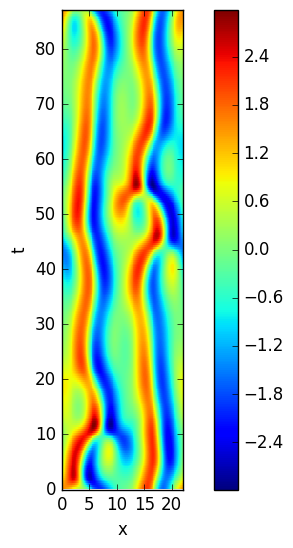
\includegraphics[width=\textwidth,height=.32\textheight]{MNG_ppo10_init}
\end{minipage}
\begin{minipage}[height=.32\textheight]{.5\textwidth}
\centering \small{\texttt{(b)}}
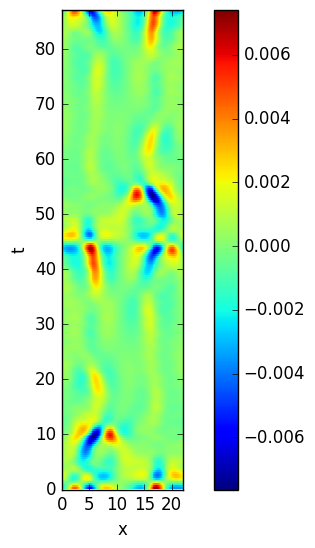
\includegraphics[width=\textwidth,height=.32\textheight]{MNG_ppo10_init_SRtest}
\end{minipage}
\begin{minipage}[height=.32\textheight]{.5\textwidth}
\centering \small{\texttt{(c)}}
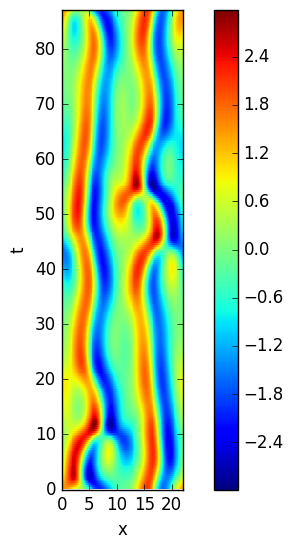
\includegraphics[width=\textwidth,height=.32\textheight]{MNG_ppo10_final}
\end{minipage}
\begin{minipage}[height=.32\textheight]{.5\textwidth}
\centering \small{\texttt{(d)}}
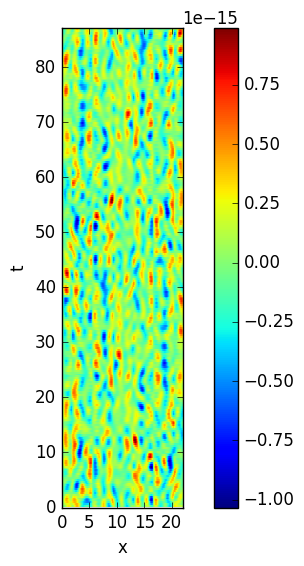
\includegraphics[width=\textwidth,height=.32\textheight]{MNG_ppo10_final_SRtest}
\end{minipage}
\caption{ \label{fig:MNGSRppo10fixed}
(a) Spatiotemporal $u(\conf,\zeit)$ generated via time integration of
\PPOtwot{22}{43.6}.
(b) The difference between (a) and its shift-reflection
(c) The resulting spatiotemporal fixed point after passing (a) through direct-matrix code,
$L_f=22.0004274064$, $T_f=87.2203435133$.
(d) The difference between (c) and its shift-reflection.
}
\end{figure}

The finite difference calculation that is used to approximate the matrix
vector product is just too inaccurate to be of use for the spatiotemporal
problem. Comparing the norms of the two vectors, the exact product, $|J \delta \mathbf{x}|$,
and its approximation,
$|\frac{F(x+\delta \mathbf{x})-F(x)}{|\delta x|}|$ they're off by almost exactly $|\delta x|$,
which makes me feel like I had made some stupid mistake but changing this in the GMRES code
makes it completely worthless.

I believe the best pursuit is going to be use matrix-free methods on the front end of
the calculation and then pass the possible solution to least-squares Newton, explicit
matrices and all unless I can find another matrix-free calculation that is more accurate
than finite-difference arnoldi inside of the GMRES routine.

Just because I believe it will work I am going for the first option. Automate my
code so that it produces initial conditions in the various subspaces, runs them through
the adjoint descent method, and if a tolerance is reached it then solves the Newton's
method equation by explicit construction of the linear system.

\begin{figure}
\begin{minipage}[height=.32\textheight]{.5\textwidth}
\centering \small{\texttt{(a)}}
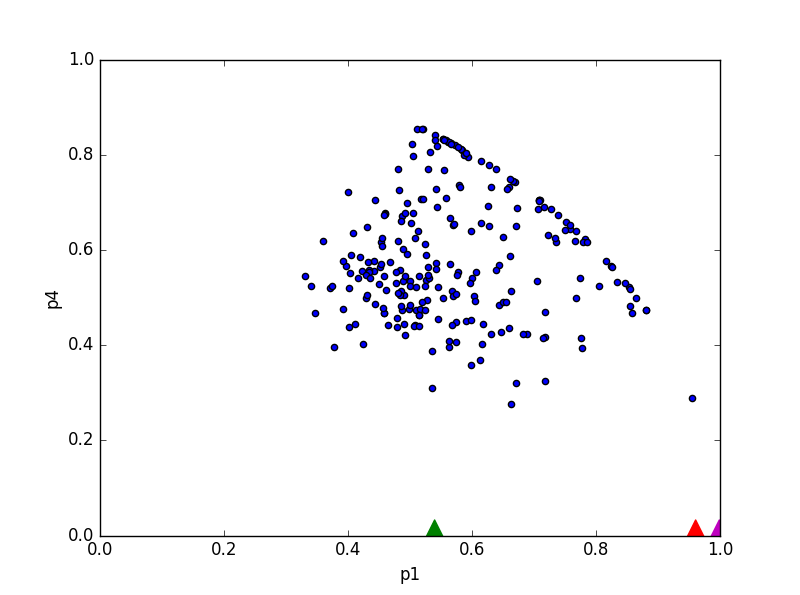
\includegraphics[width=\textwidth,height=.32\textheight]{MNG_P1P4}
\end{minipage}
\begin{minipage}[height=.32\textheight]{.5\textwidth}
\centering \small{\texttt{(b)}}
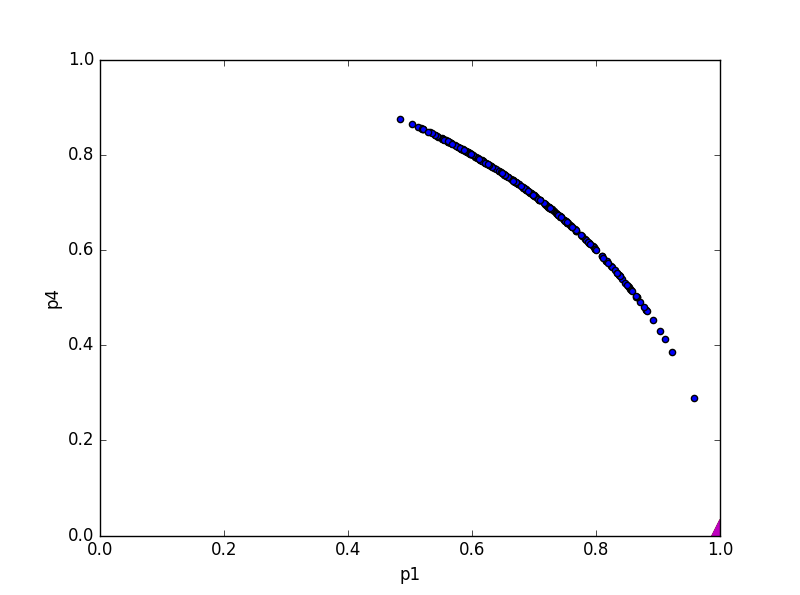
\includegraphics[width=\textwidth,height=.32\textheight]{MNG_P1P4_proj}
\end{minipage}
\caption{ \label{fig:MNGSRorganization}
Organization of \ppo\ solutions from $L=22$ domain projected into two dimensions using projection operators that form the shift-reflect subspace. The horizontal axis is defined by $P_1 = \frac{|u^{++}|}{|u|}$ , and the vertical axis
is defined by $P_4 = \frac{|u^{--}|}{|u|}$.
(a) Time integrated \ppo\ s (blue dots) and equilibria
(triangles: (red,green,magenta) for (first,second,third) \eqva\ )
(b) Projecting all solutions onto the $\bbU^{++} \oplus \bbU^{--}$ shift reflect subspace and then plotting using the same axes.
}
\end{figure}

He suggested that I look at the (time) Floquet multiplier spectrum as he believes
I might be finding periodic orbits at saddle-node bifurcations. I tried
to test this quickly but numerical underflow prevents me from seeing such
things unless I implement the algorithm from Ding and Cvitanovi{\'c}\rf{DingCvit14},
 I believe.

Much more work on automation code, just finding small inconsistencies
from testing, working on converging the \ppo\ \twot\ solutions from
Xiong's main \texttt{h5} file before moving onto randomly generated initial
conditions. The main idea from this kind of testing is namely,
to see if there are any errors in the automation code, but also see the
number of points needed for faithful time discretizations; the \ppo\ solutions
are numbered based on their temporal periods in the file so I'm hoping that
after some number that either the code will fail or not look accurate, because
I am using a 32-by-32 space-by-time discretization for all of the initial conditions.

Qualitatively, it seems that 32 points in time, (16 real valued modes) works well
up until $2\,T_{ppo}=140$ solutions, depending on the different structures present.
Convergence with this same number of modes can be achieved for periods larger than this,
so I will have to take an in-depth look at the spatiotemporal spectra to see if there is anything
discernable about these solutions.

For a variety of domain sizes and periods, I will slowly increase the length until I cannot
find anything (as described by a number of failed trials) that converges.

As my code allows for any additive factor of two increase
in the discretization size in either time or space, I'll have to describe the quantitative
way to increase said discretizations in an orderly manner. At each new starting domain length,
I will have a minimum number of spatially discretized points, and then gradually increase the
temporal discretization as the numerics seem fit. I.e., there will be a systematic description
to the growth of the discretizations instead of just multiplicative factors of two, because
this grows too quickly.

I believe I fixed all of the issues in the matrix-free \rpo\ code so now all that is left
before the computers can take over is to do testing on the initial condition generation from
a modulated spatiotemporal tile, and  seeing
if there is any way I can weigh the cost functional to penalize moving towards the $\bbU^{++}$
symmetry invariant subspace where \eqva\ live.

Otherwise other than perhaps some small efficiency, notational changes,
and antisymmetric subspace $\bbU^+$ codes the only thing left on the
table are the notions of spatiotemporal stability on compactified
spacetime and why the methods are picking out certain solutions.

As far as I'm concerned domain size and periodic
boundary conditions seemed to be axiomatic. Why attempt to perform
periodic orbit theory on the \KSe\ with $L=22$ instead of $L=22.030238210398$? My main
point is to elucidate this grievance that I just can't seem to get through to Burak.

The conventional applications of the periodic orbit theory to \KS\ start by
\textit{a priori} fixing the domain size.
What I am suggesting is that instead we let the equations themselves
dictate the periodic domain sizes which satisfy the \KS\ spatiotemporally.

Another argument is, sure, the
solutions \emph{might} (as there might be a breakdown or some other bifurcation)
be able to be continued in domain size using pseudo arc length continuation; but isn't
the whole reason behind this project due to the lack of advancement in the theory of turbulence
calculations and periodic orbit theory on large computational domains anyway?

It is hard to see how various \eqv\ solutions are related to each other from
the color-coded plots. Perhaps plotting them inside the cube Fig.~5.1\,(d) of
Cvitanovi{\'c}, Davidchack and Siminos\rf{SCD07}, reproduced here as
\reffig{SCD07f:KS22Equil}, is informative?

For $E>0$ \eqva\ and \reqva\ are organized by the {\eqv} points of
\refeq{SCD07eq:stdks}
\beq
c_{+}=(\sqrt{E},0,0)\,,\qquad c_{-}=(-\sqrt{E},0,0)
\,,
\ee{EqvEqvPts}
as explained in ChaosBook\rf{CBook:PDEs}, Example~30.6. {\em Equilibria of
equilibria.}

Now rescale $u$ in \refeq{SCD07eq:stdks} as
\(u \to u_p\sqrt{\expctE_p}\):
\beq
{\textstyle\frac{1}{2}}u_p^2
    + \frac{1}{\sqrt{\expctE_p}} (- c u_p + u_{p,x} + u_{p,xxx})=1
\,,
\label{rescal:eq:stdks}
\eeq
The {\eqv} points of \refeq{SCD07eq:stdks} are now
\beq
c_{+}=(1,0,0)\,,\qquad c_{-}=(-1,0,0)
\,,
\ee{EqvEqvPtsRsc}
so all \reqva\ should line up nicely, like
ducks in a row.
You can do the same thing for any \twot\ $p$ by rescaling the \KSe\ \refeq{e-ks}
by the \twot\ $p$ energy density \refeq{twotEnergy}.

I do not remember Lan and me doing this, but it looks like the symbolic
dynamics for all \eqva\ and \reqva\ could be a $\pm$ for each turn around the
stable manifold of $c_{\pm}$.

Currently running testing to determine how many spatiotemporal modes are needed for accurate representations of
{\twots}. Running tests where $L=23$ with the number of spatial modes is $m=16$ which
has been shown before to be adequate at this domain size. Although I have code running I have yet to find to most
convincing way of demonstrating where the temporal discretization is adequate, convergence doesn't seem to be the
best means of demonstrating this because solutions can converge with a small temporal discretization but when
viewed qualitatively sometimes even the converged solutions do not look like what I would expect.

After further testing, imposing the correct spatial scale as determined by the spectrum of the \KSe\
$\tilde{L} = 2\pi \sqrt{2}$ leads to many \eqva\ solutions so imposing the incorrect spatial scale is almost more
beneficial much like imposing a larger than normal magnitude of the spatiotemporal field $u(x,t)$.

Extracted information from \refref{Canuto88} on what I thought was one of the gaps in my code
which was the fact that it seemed to perform much better as a fully aliased pseudospectral
calculation rather than a de-aliased calculation. I feared that this would bring criticism
so as I tried to armor myself by actually \emph{reading}. My argument is that while aliasing
can be devastating for temporal evolution due to the contamination of the higher Fourier
mode components by their aliases, ($k' = k + N$) where $N$ is the number of collocation
points, the spatiotemporal problem should be fine as long as the calculation is well
resolved enough. In fact, this is likely why I have solutions that "converge" on larger
spatial domains than the discretizations can seem to resolve.

Aliasing commments:
\begin{quote}
For evolution problems  one must address the issue of the temporal numerical
stability of the calculation. Collocation approximations must be formulated
with more care than Galerkin approximations. The reason is that for evolution
problems with quadratic conservation properties, the Galerkin formulation
will automatically yield semi-discrete quadratic conservation laws.
\end{quote}

\begin{quote}
Numerous comparisons have been performed for aliased and de-aliased
calculations of the periodic, multidimensional Navier-stokes equations.
Useful discussions may be found in
\rf{Orszag72,FoxOrs73,Montigny82,Kerr85}.  All of these authors conclude
that with sufficient resolution, aliased calculations are quite acceptable.
\end{quote}


\begin{quote}
Moser, Moin and Leonard\rf{MML83} caution against aliased calculations.
They present a single, poorly resolved, aliased calculation and compare it with three
de-aliased calculations, one poorly resolved, one moderately resolved, and one well
resolved. Their single aliased result is certainly much worse than their well resolved,
de-aliased case, but their poorly resolved, de-aliased case is no better than the aliased
one. Hence, their conclusion is not supported by their evidence.
\end{quote}

In light of these comments and discussions I believe that de-aliasing is more
important in the context of accurate temporal evolution, but not required in
the spatiotemporal fixed point problem as long as the patterns are
sufficiently resolved. One way of thinking about this is that in the
discretization of the spatiotemporal \KSe\ we could add a term that
represents the aliasing,
\[
\sum_{m',n'}\sum_k\neq 0,j\neq 0 a_{m-m'+kM,n-n'+jN}a_{m+kM,n+jN}
\,,
\]
as it is implicit in the fully aliased representation of the equations.

I believe the spectrum of the \KSe\ plays a role, and it might be wise to at
least dealias the temporal convolution sum as there is less of a precedent
for ignoring it; In the spatial case we can at least claim the hyperdiffusion
term diminishes the amount of corruption in the spatial wave number, but this
is harder to motivate for the temporal terms.
More motivation from Canuto, Hussaini, Quateroni and Zhang\rf{Canuto88} are
their fig.~7.1 and fig.~7.4, where the fully aliased but more resolved terms seem
to beat out even the dealiased computations in energy conservation of the KdV
equation for fig.~7.1.
Their fig.~7.4 is a reproduction of the effects of aliasing in the transition
to turbulence in channel flow by  Krist and Zang\rf{KrZa87}. Only the high
resolution (aliased) seems to be physically representative of the actual
solution, and even the dealiased computation on a coarser discretization
(while better than the equivalent aliased discretization) still does not
prevent artificial oscillations. This is also a temporal evolution problem
which we are not dealing with.

I believe I found the minimal hook and streak patterns (or at least
members of the same families) today. This was accomplished by using the
hybrid-methods that I used to trawl. Previously, I was only using
Gauss-Newton to converge subdomains as it worked but the hook required
adjoint descent before applying Gauss-Newton in order to converge.

Solution hook = \emph{rpo\_L13.07\_T10} was found by using a family
member of the shortest \ppo\ in time at $L=22$ whose energy was a local
maximum. This ended up being at $L=20$, but this turns out to not matter.
What matters in the end is that I use hybrid methods and not just
Gauss-Newton to try to converge the tiles; just like how I had done for
all of the {\twots} beforehand. The expedient results of
just using Gauss-Newton and finding ``defects" and ``gaps" had led me
astray.

Similar story to that of the hook; applying hybrid numerical methods
allowed me to find an \eqv\ solution whose spatial extent is
approximately $2\pi$, or $\pi$ in the fundamental domain of the
antisymmetric subspace $\bbU^+$.

Numerical continuation of the hook and gap solutions provide continuous
families of solutions of which it seems the Predrag is correct that the
``defect" type solution and ``hook" type solution are of the same family.
As a means of trying to identify some criterion by which to choose
members of said families I produced plots of members of the continuous
families adjacent to plots of the entire family's energy, spatiotemporal
averaged energy dissipation and production. There is some slight
numerical discrepancy but they should be equal in theory; It could be the
quadrature rule that I am using to calculate $<u_{\conf\conf}^2>_{L\period{}}$
and $<u_{\conf}^2>_{L\period{}}$, where $< \star >_{L\period{}}$ indicates
spatiotemporal average.

I thought it might be possible to identify each family by picking out the
constitutive member that had maximal or minimal dissipation and
production values; but for the numerical continuation of the gap solution
there doesn't seem to be any local maxima or minima. The benefit of this
type of analysis is that while there isn't any local maxima or minima for
the gap family, as I increase $L$ to its upper limits (in terms of being
able to converge the solution) the period of the solution grows extremely
quickly; in my mind making it more and more of an isolated solution. The
reason I hold this belief is that if we contemplate the family of gap
solutions in the context of the \KSe\ as a dynamical system, an
incredibly long period in this instance is actually prohibitive due to
the fact that the antisymmetric subspace $\bbU^+$ is a flow invariant
subspace. The idea I have is that the it is possible for \po 's to shadow
generic trajectories but as the period increases, it is essentially a
statement akin to ``the trajectory stays near the flow invariant subspace
for longer and longer periods of time" which (although I hesitate to use
this word) probabilistically doesn't seem likely.

In summary I suppose my thinking is that due to the fact that
antisymmetric \po 's lie in a flow invariant subspace $\bbU^+$ that
trajectories can neither leave nor enter then the period is a sort of
measure of how isolated these \po 's must be. In this regard I think that
the more relevant quantities would be a respective densities of scalar
quantities than the quantities themselves (average energy, dissipation,
etc.).

The numerical continuation of defect1 = \emph{rpo\_L13.2\_T15}  tile,
\reffig{fig:MNG_ppo_subdomains}\,(b), the first tile I entitled 'defect'
seems to be a member of the family of the reflection of the ``hook"
family: they are the same family up to discrete symmetry. My attempt
to demonstrate this is to take three representatives of each family in
\reffig{fig:MNG_leftright_family}, and show that at similar
spatiotemporal domains the solutions look very similar up to spatial and
temporal translations.
In this respect, one can see the family progresses from ``defect"
 to ``hook" to \reqv\, as $\tilde{L}$ increases.

My thought process on how to interpret this family goes as follows:
I don't know whether to interpret the ``hook" as a transition describing
breakdown of the \twot\ into a \reqv, or maybe as ``spatiotemporal
heteroclinic connection" but I am unsure if such a statement makes sense
in the absence of dynamics. Therefore I thought that maybe it makes sense
in terms of spatiotemporal symbolic dynamics. If one was playing sudoku
with spatiotemporal symbolic dynamics and there were symbols for defect
and \reqv, I think ``hook" would be a symbol that could fit in the
middle. Now, this doesn't really make sense because $\text{hook}\equiv
\text{defect}$ because they are members of the same family; it just gets
too complicated too quickly to extrapolate any ideas currently, much more
work required.

\begin{figure}
\begin{minipage}[height=.18\textheight]{.30\textwidth}
    \centering \small{\texttt{Defect1}}
    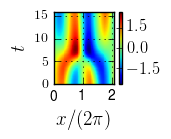
\includegraphics[width=\textwidth,height=.14\textheight]{MNG_rpo_L13d2_T15}
\end{minipage}%
\begin{minipage}[height=.18\textheight]{.30\textwidth}
\centering \small{\texttt{(a)}}
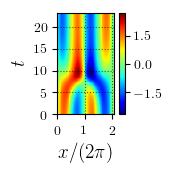
\includegraphics[width=\textwidth,height=.20\textheight]{MNG_rpo_L12p996_T23}
\end{minipage}%
\begin{minipage}[height=.18\textheight]{.30\textwidth}
\centering \small{\texttt{(b)}}
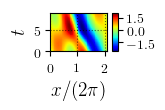
\includegraphics[width=\textwidth,height=.13\textheight]{MNG_rpo_L13p096_T8}
\end{minipage}%
\begin{minipage}[height=.18\textheight]{.30\textwidth}
\centering \small{\texttt{(c)}}
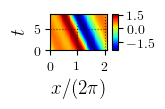
\includegraphics[width=\textwidth,height=.13\textheight]{MNG_reqv_L13p106_T8}
\end{minipage}
\\
\begin{minipage}[height=.18\textheight]{.30\textwidth}
    \centering \small{\texttt{hook}}
    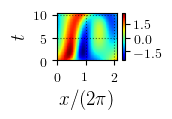
\includegraphics[width=\textwidth,height=.13\textheight]{MNG_rpo_L13p07_T10}
\end{minipage}%
\begin{minipage}[height=.18\textheight]{.30\textwidth}
    \centering \small{\texttt{(d)}}
    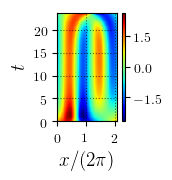
\includegraphics[width=\textwidth,height=.20\textheight]{MNG_rpo_L12p995_T23}
\end{minipage}%
\begin{minipage}[height=.18\textheight]{.30\textwidth}
    \centering \small{\texttt{(e)}}
    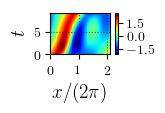
\includegraphics[width=\textwidth,height=.13\textheight]{MNG_rpo_L13p095_T9}
\end{minipage}%
\begin{minipage}[height=.18\textheight]{.30\textwidth}
    \centering \small{\texttt{(f)}}
    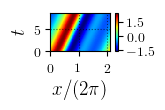
\includegraphics[width=\textwidth,height=.13\textheight]{MNG_reqv_L13p105_T8}
\end{minipage}
\caption{ \label{fig:MNG_leftright_family}
(a) \twoT\ \emph{rpo\_L12.996\_T23},
(b) \twot\ \emph{rpo\_L13.096\_T8},
(c) \reqv\ \emph{reqv\_L13.106\_T8}.
These three solutions were produced by numerical continuation in spatial
domain size of \twot\ defect1 = \emph{rpo\_L13.02\_T15}  tile
(see  \reffig{fig:MNG_ppo_subdomains}).
(d) \twoT\ \emph{rpo\_L12.995\_T23},
(e) \twot\ \emph{rpo\_L13.095\_T8},
(f) \reqv\ \emph{reqv\_L13.105\_T8}.
These three solutions were produced by numerical continuation in spatial
domain size of \twot\ hook = \emph{rpo\_L13.07\_T10} tile.
\twoTs\
(a) \emph{rpo\_L12.996\_T23} and
(d) \emph{rpo\_L12.995\_T23}
are the one and the same $\PO{(13.0,23)}\in\bbU^+$, differing only by
relative space and time shifts. The reflection symmetry is broken by the
nearby solution drifting either to the left or to the right, so (e,f)
belong to the right-drifting reflection of the left-drifting branch of
the solutions (a,b), \ie, they belong to the same branch of the
solution after the reduction of the spatial reflection symmetry.
In general, solutions can be distinguished or identified only after they
are sectioned and sliced, as done in \reffig{fig:MNG_hookequalsdefect}.
}
\end{figure}

\begin{figure}
\begin{minipage}[height=.32\textheight]{.8\textwidth}
\centering \small{\texttt{(a)}\qquad\qquad\texttt{(b)}}
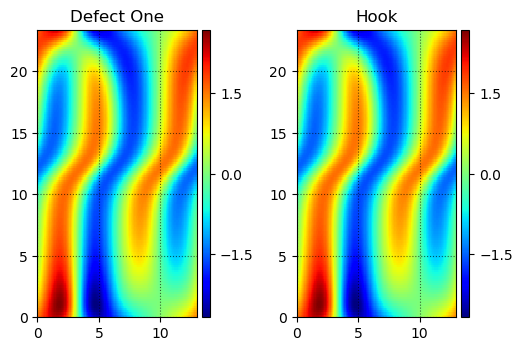
\includegraphics[width=\textwidth,height=.32\textheight]{MNG_hookequalsdefect}
\end{minipage}
\caption{ \label{fig:MNG_hookequalsdefect}
Continued from \reffig{fig:MNG_leftright_family}.
Sliced and sectioned minimal \twot\ solutions (not scaled relative to
others in repository; horizontal axis is $L$);
(a) Defect1 = \RPOtwot{13.2}{15} %\emph{rpo\_L13.2\_T15}
tile,
\reffig{fig:MNG_ppo_subdomains}\,(b), numerically continued to
$(\speriod{},\period{})=(12.996,23.373682)$.
(b) Reflection of the hook  = \RPOtwot{13.07}{10} %\emph{rpo\_L13.07\_T10}
tile numerically
continued to $(\speriod{},\period{}) = (12.996,23.373670)$.
}
\end{figure}

\begin{figure}
\begin{minipage}[height=.20\textheight]{.8\textwidth}
\centering \small{\texttt{(a)}}
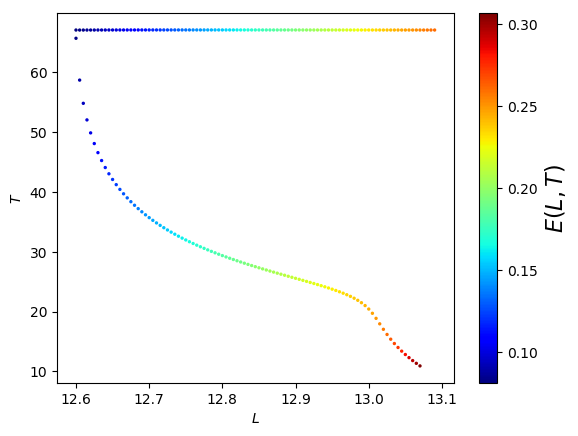
\includegraphics[width=\textwidth,height=.32\textheight]{MNG_hook_space_cont}
\end{minipage}
\caption{ \label{fig:MNG_hook_spatial_cont}
Bifurcation diagram plotted in $(\speriod{},\period{})$ plane.
Two branches resulting from numerical continuation in $L$ of
the hook  = \RPOtwot{13.07}{10} %\emph{rpo\_L13.07\_T10}
tiles family. $L$ was decreased until the
Gauss-Newton method failed; at which point, the numerical continuation
began increasing $L$ to test for hysteresis. This can be seen by the fact
that the bifucation diagram has two branches.
}
\end{figure}

\begin{figure}
\begin{minipage}[height=.20\textheight]{.8\textwidth}
\centering \small{\texttt{(a)}}
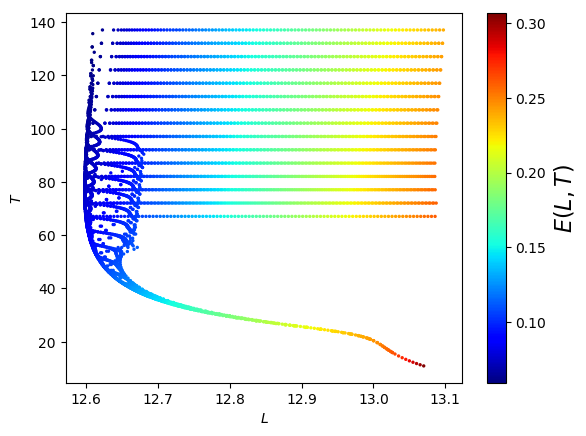
\includegraphics[width=\textwidth,height=.32\textheight]{MNG_st_cont}
\end{minipage}
\caption{ \label{fig:MNG_hook_st_cont}
Bifurcation diagram plotted in $(\speriod{},\period{})$ plane; numerical continuation of all points in \reffig{fig:MNG_hook_spatial_cont}.
These points were acquired by increasing $T$ and then decreasing $T$ via numerical continuation of both the lower and upper spatial continuation branches. The step size that $T$ was changed by was $\Delta T = 5$; smaller step sizes and smaller ranges seem to indicate that each branch is a one dimensional family.
}
\end{figure}

\begin{figure}
\begin{minipage}[height=.20\textheight]{.8\textwidth}
\centering \small{\texttt{(a)}}
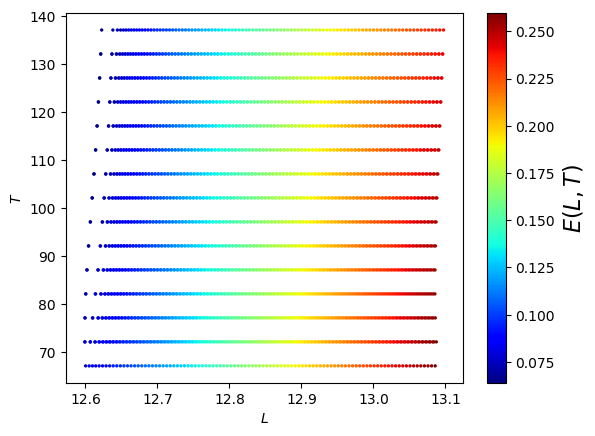
\includegraphics[width=\textwidth,height=.32\textheight]{MNG_upper_dT5}
\end{minipage}
\caption{ \label{fig:MNG_upper_dT5}
Bifurcation diagram plotted in $(\speriod{},\period{})$ plane; numerical continuation of upper branch of \reffig{fig:MNG_hook_spatial_cont}.
These points were acquired by increasing $T$ and then decreasing $T$ via numerical continuation of the upper spatial continuation branch. The step size that $T$ was changed by was $\Delta T = 5$; smaller step sizes and smaller ranges seem to indicate that each branch is a one dimensional family.
}
\end{figure}


\begin{figure}
\begin{minipage}[height=.20\textheight]{.30\textwidth}
\centering \small{\texttt{(a)}}
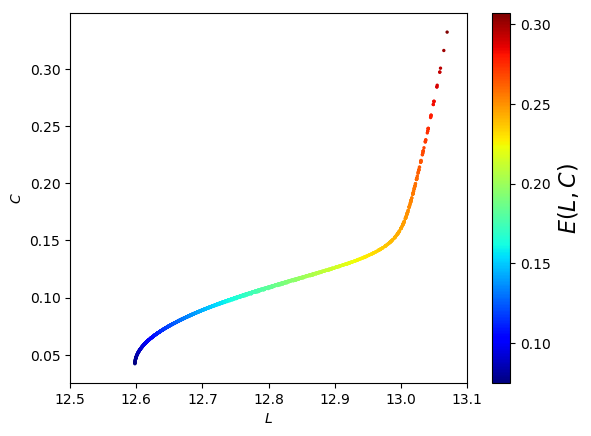
\includegraphics[width=\textwidth,height=.16\textheight]{MNG_LC_dT1}
\end{minipage}
\begin{minipage}[height=.20\textheight]{.30\textwidth}
\centering \small{\texttt{(b)}}
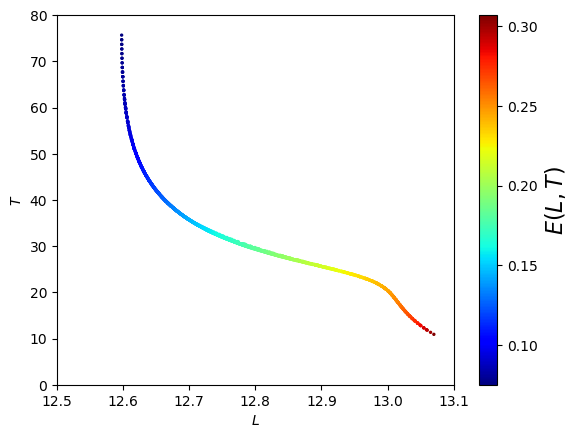
\includegraphics[width=\textwidth,height=.16\textheight]{MNG_LT_dT1}
\end{minipage}
\begin{minipage}[height=.20\textheight]{.30\textwidth}
\centering \small{\texttt{(c)}}
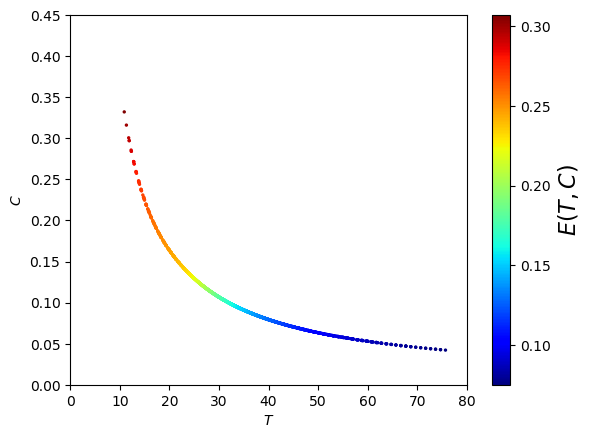
\includegraphics[width=\textwidth,height=.16\textheight]{MNG_TC_dT1}
\end{minipage}
\caption{ \label{fig:MNG_lower_dT1}
Numerical continuation of the lower spatial continuation branch of
\reffig{fig:MNG_hook_spatial_cont} by decreasing $T$ by 10 with step
sizes of $\Delta T = 1$. Plots in (a)$(L,C)$ plane (b) $(\speriod{},\period{})$ plane
(c) $(T,C)$ plane. Spatiotemporal energy is color coded.
}
\end{figure}

\begin{figure}
\begin{minipage}[height=.20\textheight]{.30\textwidth}
\centering \small{\texttt{(a)}}
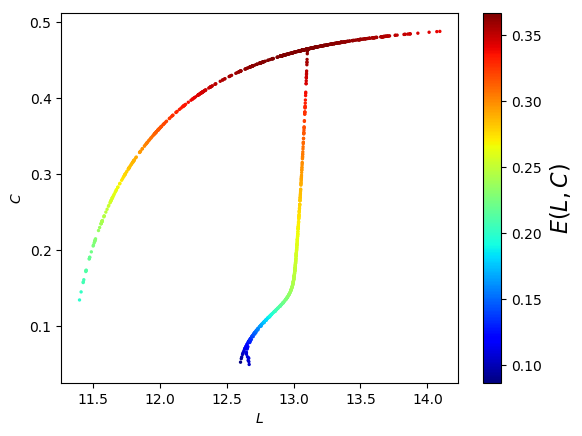
\includegraphics[width=\textwidth,height=.16\textheight]{MNG_LC_dT5}
\end{minipage}
\begin{minipage}[height=.20\textheight]{.30\textwidth}
\centering \small{\texttt{(b)}}
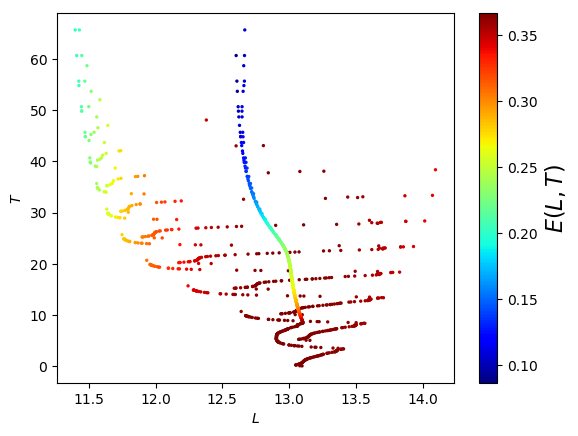
\includegraphics[width=\textwidth,height=.16\textheight]{MNG_LT_dT5}
\end{minipage}
\begin{minipage}[height=.20\textheight]{.30\textwidth}
\centering \small{\texttt{(c)}}
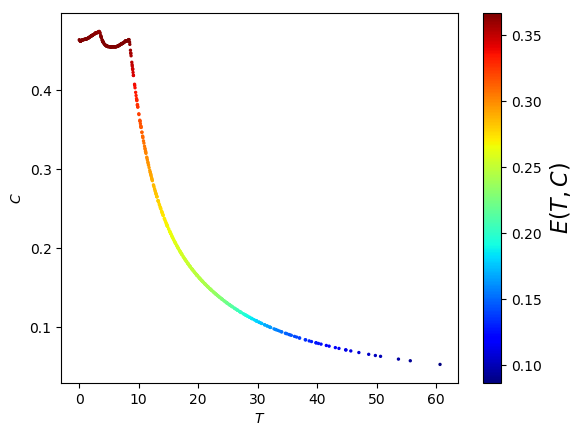
\includegraphics[width=\textwidth,height=.16\textheight]{MNG_TC_dT5}
\end{minipage}
\caption{ \label{fig:MNG_lower_dT5}
Numerical continuation of the lower spatial continuation branch of
\reffig{fig:MNG_hook_spatial_cont} by decreasing $T$ by as much as possible
(while still remaining positive) with step
sizes of $\Delta T = 5$. Plots in (a) $(L,C)$ plane, (b) $(\speriod{},\period{})$ plane, and
(c) $(T,C)$ plane. Spatiotemporal energy is color coded.
}
\end{figure}

\PCpost{2018-08-22}{
Matt's trial run of the thesis proposal presentation.
Matt, can you complete these notes?
\begin{itemize}
  \item Burak: Summarize in intro how people used to do this traditionally in
turbulence (past 20 years). You are developing a statistical mechanics approach
to spatiotemporal states in terms of building blocks.
  \item Burak: emphasize the bridge between small structures and large domains.
Similar to homogenous turbulence in large cube.
  \item John: shorten introductory ``what am I going to do?''
  \item Burak: Can do this visually - will also save time.
  \item Burak: can go through slides faster. When you name a symmetry, give a picture,
the picture will explain it.
  \item Burak: in slide of \twots, put pictures of examples.
  \item Burak: in \KS\ slide need b.c.'s, explain terms by annotating the
  equation, make comparison to Navier-Stokes.
  \item Burak: \rpo s; moves with mean speed
  \item Burak: write what symmetry a given solution has
  \item Burak: brag about your domains being much larger than $L=22$
  \item Spatial scale  $\sqrt{2}$ comes from competition of unstable diffusion and
stable hyperdiffusion. John: Where does the time scale comes from? Predrag:
one scale is the Lyapunov time of $\approx 0.4$ for the current scale conventions.
I think it has nothing to do with the actual time scale.
  \item John, Predrag: generate a few large spacetime domain solutions, look at
magnitudes of
\\
(1) spatial Fourier components, averaged over time - should peak at
$k_{max}=2\pi/\sqrt(2)$, fall off exponentially for large wave numbers.
\\
(2) time Fourier components, averaged over space - does it peak anywhere?
does it have a shoulder, beyond which it fall off exponentially for large frequencies?
  \item Predrag Xiong and predecessors work on \KS\ inertial manifolds should
serve as a guide here. Correctly scaled spectra (dimensions scales linearly with $L$,
for example) all fall on the same curve.
  \item John: How are you going to do tilings? By Photoshopping?
  \item Matt: I'll start with my symbolic dynamics - from a given symbol array I'll
generate approximate solution by corresponding tiles, the anneal it.
        \MNGedit{Patterns whose boundaries are very different (in some norm)
        might serve to help with grammar.}
  \item Burak: emphasize your success - your solutions are robust. Already achieved
the qualitative confirmation that large solutions can split into small domains.
  \item John: Inability to use Newton-Krylov methods sounds wrong; in his
  experience cost functions are relatively smooth in all parameters.
  \MNGedit{I suppose if I'm not including calculations, numerical
  evidence, etc., I should just not bring topics up; better to focus on
  other details.}
  \item Include figures that show initial conditions and the solutions
  they converge to. Also show how a ``random'' looking initial condition
  can converge but a ``good-looking'' (looks close to \KS\ solution)
  initial condition can fail.
  \item Ashley: Don't necessarily have to look at minimal {\twots} as library of converged solutions are technically all
  ``tiles'' as well just of larger size.
  \item Burak: Numerical continuation of library of solutions can serve
  to flush out spatiotemporal \twots.
\end{itemize}
}

\item[Andre Wibisono Talk]
Universal language for describeing phenomena,
Learning, economoics, Optimal Transport, Neuroscience, Statistical mechanics,
statistics,biology,physics (Laws of physics as principle of least action in spacetime).
Find best parameter $x$ that minimizes some loss function. (cost function).

Convex Optimization in $\mathbb{R}^n$ in continuous and discrete time. Want to
design ``fast'' algorithms to solve $\min f(x)$. Assuming differentiability, convexity,
gets us a guarantee on convergence properties of the different methods.

Many algorithms are discretizations of dynamics in continuous time, for example
gradient descent and gradient flow. Talking about convergence rates, differences
between continuous and discrete time.

Gradient descent
\beq
x_{k+1} = x_k - \epsilon \nabla f(x_k)
\eeq

Gradient Flow
\beq
\dot{X}_t = -\nabla f(X_t)
\eeq

Nice properties for convex, nonconvex f, some conditions on bounded $\nabla^2 f$.
Can say a lot about convergence.

\beq
x_{k+1} = x_k -\epsilon \nabla f(x_k)
\eeq

Theorem: If $f$ is convex and $\frac{1}{\epsilon}$ smooth then gradient descent scales like
$\mathcal{O}(\frac{1}{\epsilon k})$

\beq
\dot{X}_t = -\nabla f(X_t)
\eeq

Theorem: If $f$ is convex (upper bound on Hessian) then gradient descent scales like
$\mathcal{O}(1/(t))$.

\ie these have same convergence rates if $t = \epsilon k$.

How to design (provably) fast dynamics for $\min f$. Can we get faster than gradient
flow? What is the \emph{fastest} dynamics? Not actually well defined, definition of
\emph{fast} is dependent on $t$ parameterization; reparameterizing
via speeding up time speeds up algorithm.

The sped up gradient flow $\tau = \frac{t^{p-1}}{p-1}$ (specific form dependent on convex
$f$ then gradient flow takes

\beq
\dot{Y}_t = -t^{p-2}\nabla f(Y_t)
\eeq

What is sped-up gradient descent?
\beq
y_{k+1} = y_k - \epsilon k^{p-2}\nabla f(y_k)
\eeq

This does not get better than $\mathcal{O}(1/k)$
Faster dynamics from optimization,
Recaling gradients
\beq
\dot{X}_t = -\nabla f(X_t)/||\nabla f(X_t)||^{\frac{p-2}{p-1}}
\eeq

Acceleration and speeding up time.
\beq
\ddot{X}_t + \frac{p+1}{t} \dot{X}_t + t^{p-2}\nabla f(X_t)=0
\eeq

First, look at rescaled gradient flow

\beq
\dot{X}_t = -frac{\nabla f(X_t)}{||\nabla f(X_t)||^{\frac{p-2}{p-1}}} = arg min ( <\nabla f,v > + 1/p ||v||^p )
\eeq

Faster when the gradient is small. (This might be worth looking at).

$p = \infty$ is ``normalized gradient flow''.

Convergence $\mathcal{O}(frac{1}{t^{p-1}})$. Same as gradient flow when $p=2$.
Proof provided by convexity and Fenchel-Young.

He is skipping details to get to accelerated flow. How to implement
as an algorithm. Proximal method, Higher-order gradient descent, rescaled gradient descent.
Proximal is an implicit method (backwards discretization of rescaled gradient).

\beq
x_{k+1} = arg min { f(x) + \frac{1}{\epsilon p} ||x-x_k||^p}
\eeq

\beq
x_{k+1} = arg min { f_{p-1}(x;x_k) + \frac{1}{\epsilon p} ||x-x_k||^p}
\eeq

Instead of minimizing $f$, minimize the taylor expansion up to terms $p-1$ order.
Examples of this are, $p=2$ leading to regular gradient descent, $p=3$ Cubic newton.

Assumption that f is smooth of order $p$ then convergence rate is
$\mathcal{O}(\frac{1}{\epsilon k^{p-1}})$.

New stuff. If function is \emph{strongly smooth} (all gradients up to $p$th order smooth), then,

\beq
x_{k+1} =x_k -\epsilon^{\frac{1}{p-1}} \frac{\nabla f(X_t)}{||\nabla f(X_t)||^{\frac{p-2}{p-1}}}
\eeq

Proximal method. Higher gradient descent. Rescaled gradient descent. Lower bound given
by Nemirovski, Yudin, Nesterov. Using assumption that algorithm generates $x_k \in x_0 +
Lin(\nabla f(x_0),\cdots,\nabla f(x_k))$. This has order $\mathcal{O}\frac{1}{\epsilon k^2}$

Rescaled gradient and cubic-regularized require that Hessian is bounded but we can get
better without this assumption with the accelerated gradient descent.


\textbf{Accelerated Descents}
\bea
x_{k+1}&=& y_k - \epsilon \nabla f(y_k) \continue
y_k &=& x_k + \frac{k-1}{k+2}(x_k-x_{k-1})
\eea

gradient descent ``with momentum''.
function value can oscillate, gradient descent is monotonic. Achieves
optimal convergence rate.

Gradient descent is very intuitive, but it is not optimal.
Now let's go to continuous time limit,
\beq
dd x_t + 3/t dot xt + \nabla f(x_t)=0
\eeq

For accelerated gradient descent (AGD). Can show that oscillatory dynamics both
in function value and trajectory. Convergence rate proofs via Lyapunov function.
Question, whhy the dynamics, why the optimality. There is non constant damping.
With $1/t$ damping for convex f and constant damping for strongly convex f. (strongly
convex is bounded Hessian).

How would you come up with this? Use a lagrangian formulation that generates
almost all of the algorithms that we know.
Lagrangian, principle of least action, optimal curves satisfy Euler-Lagrange equation.

Lagrangian that he uses:
\beq
L(x,v,t) = t^3(1/2||v||^2 - f(x))
\eeq
Reference to Yezzi talk from last week ``Accelerated optimization of PDE framework''.
If we speed up time in the AGD then it has $\mathcal{O}(1/t^p)$. Can we implement this?
not quite he says. Reference to Bregman divergence; working on Euclidean space with
metric given by the Hessian. Write the NGF as ``mirror flow''
\beq
\cdot \nabla h(x_t) = -\nabla f (x_t)
\eeq
can be discretized as mirror descent (MD) as
\[
x_{k+1} = \mbox{arg min}_{x\in R^n} \{ <\nabla f, x-x_k>
         + \mbox{Bregman divergence term} \}
\,.
\]
Accelerated mirror descent by Nesterov (2005).
Can ask, what is Lagrangian for accelerated mirror flow (AMF)?
\beq
\ddot{} x_t + 3/t dot xt + (\nabla^2 h(X_t + t/2 \dot{X}_t))^{-1} \nabla f(x_t)=0
\eeq

AMF is generated by the Bregman Lagrangian.
Speeding up AMF with speed up time rescaling.

How to implement (polynomial rate AMF) Can be unstable.
Therefore borrow Nesterov's trick and indroduce an aux sequence to stabilize
the algorithm. ``What actually works'' Accelerated higher-order gradient
descent (AHGD) has correct convergence rate.

Can also accelerate rescaled gradient descent (easier). Again due to Nesterov.
AHGD is the discretized form of accelerated mirror flow.

Can convert to Bregman Hamiltonian, looks like Lyapunov function; use symplectic
structure?. Madison, Paulin, Teh, O'Donoghue, Doucet 2018 (different Hamiltonian).

What's still unclear, the Lagrangian works, but still don't know if its best.
Need to formulate optimal dynamics for optimization.

In my personal experience when looking for numerical methods
that are commonly used in nonlinear optimization procedures fall
into two classes: descent methods and iterative methods. I thought I
was pretty exhaustive on the types of numerical optimization methods
(specifically descent methods) that were out there but after this talk
I realize that I came across the most common but not the most cutting
edge. That being said, this talk
helped provide me with some of the more recent, cutting edge algorithms
in the descent method category, giving me a new list of numerical methods
I add to my numerical methods suite after sufficient time.
The list of different descent methods mentioned looks something like,

\begin{itemize}
\item proximal method
\item ``mirror prox'' method
\item higher-order gradient gescent
\item rescaled gradient descent
\item accelerated gradient descent
\item accelerated mirror descent
\item accelerated higher-order gradient descent
\end{itemize}

These are all methods I can try; in addition to these descent
algorithms I can try different direct and iterative methods as well such as,

\begin{itemize}
\item Cubic regularized Newton
\item BiCGSTAB
\end{itemize}

As opposed to the more common Newton and GMRES methods. I think
The most promising of these numerical that I can try out are the
so called accelerated methods, which use the acceleration techniques
of the past derived by Nesterov\rf{Nesterov83}
applied to newer optimization algorithms.

Implemented a number of new numerical methods to see if any of them could
compete with what I currently have. Out of the three classes of solvers,
(descent methods, direct methods, iterative methods) iterative methods
have work terribly for me. Therefore in order to see if its just my innate
disability to be able to use these methods I am running a suite of tests
using built in optimization algorithms in SciPy.

On the other numerical front, I implemented two different types of Levenberg-Marquardt
algorithms, the first one\rf{FZlevmar13} performed much better than \refref{WHlevmar84},
and much better than the BiCGSTAB algorithm I also implemented; but for whatever
reason the Gauss-Newton with back-tracking performs better in all cases I have tried
so far.

I also tried more testing with the accelerated adjoint descent that I had recently forgone
in favor of using a lower order integration scheme in fictitious time with preconditioning,
I'm thinking I'll likely stick to that as well.

The main portion of today's work was to implement the gluing algorithm that takes any
two \twot\ solutions with the same solution and glues them together, with a slough of
options as to how one specifically wants to do this, namely, whether to concatenate in
space or time, whether to pad the boundaries between the two solutions with buffer
zones, and how to smooth out the glued together data. The smoothing still needs some fine
tuning; I'm using circular convolution with an anisotropic Gaussian that is wider in the
dimension by which two solutions were glued. Currently trying to run through some test
cases. The two shortest \ppo\ solutions concatenated in time after adjoint descent
looks interesting but Gauss-Newton squashes it into an equilibrium. Definitely needs
some more fine tuning on the smoothing front.

Worked on symbolic dynamic initial condition
generation and thinking through gluing codes

The general idea is to take the library of solutions that I have found
and then automate the process that glues them together; \ie
the automation will contain the following subroutines:
\begin{enumerate}
\item Determine symmetry subgroup of the solutions.
\item Choose solutions and direction (space or time) to glue.
\item Make sure the discretizations match such that the final result
is a rectangular grid.
\item Use Fourier smoothing, Gaussian mollifiers, or insertion of
zeros to pad the two solutions and connect them or any combination
of these procedures.
\item Determine $(\speriod{},\period{},\sigma)$ based on averaging.
\item Use either hybrid adjoint-descent Newton or adjoint descent
Newton Krylov to converge the approximate solution.
\end{enumerate}

I have an inkling that liberal use of inserting streaks and traveling
wave type solutions might be used to help glue solutions together as
but I don't have motivation for this other than intuition currently.

Implement a number of various means for rediscretization,
reordered a bunch of processes.
List of rediscretization processes, ``Residual guided rediscretization'':
 Lower $N$ and $M$ while $|F|^2$ is decreasing
``Converged Solution guided rediscretization'': Lower $N$ to minimum
value dependent on period, incrementally increase until solution converges,
then do
the same with $M$.

The first of these is the cheap, expedient procedure that should
 be used to produce initial conditions that
have a smaller discretization that one started with; The second
tries is a much more expensive procedure
because it tries to find the minimal discretization for \emph{converged}
solutions; therefore, it requires
a bit of computational time. From testing it seems much better to
 increase the discretization at all points
in the calculation, and then as the very last preprocessing step,
 decrease the discretization.
The motivation for this increased cost is because the second
 procedure has repeated gluings in mind; not only
do we want a converged solution, but also the converged solution
with minimal discretization. Because the convergence
seems to be much more finicky with respect to changes in the
spatial discretization when working at a fixed
length $L=22$.

A correction was made that more fairly weights solutions
depending on their initial parameters; I was mistakenly
creating initial conditions where solutions with drastically
different periods were receiving equal number of points
in the final discretization, as opposed to being weighted by
how much they contribute to the final periods. In other
words I wasn't incorporating the correct scales in the
initial conditions.

In terms of specific testing, the main parameters that I tested were,
\begin{itemize}
\item Rediscretization before and after adjoint descent
\item The size of the discretization of the buffers
\item The method of creating the buffers
\item The use of the ``residual-guided'' rediscretization
\end{itemize}

which lead to the following conclusions. It's always better to rediscretize before
before numerical methods. A moderate buffer size is $5$, a moderate number of points and
likely should be proportional to the total number of points; still testing.
Use of the residual guided rediscretization routine should always
be used on the dimension perpendicular to the gluing dimension first.
Some (seemingly) improved lower bounds on the number of points in the discretization
is something like $M = 2^(\log_2 L + 1)$ and $N = 2^(\log_2 L -1)$.
Main point: less sensitive to changing (reducing) the maximum frequency
mode (less points in time).


\begin{figure}
\begin{minipage}[height=.30\textheight]{.6\textwidth}
\centering \small{\texttt{(a)}}\\
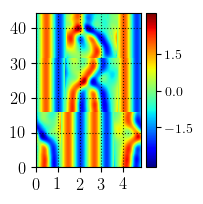
\includegraphics[width=.8\textwidth,height=.3\textheight]{MNG_ppo_tiling_init_pretruncation_1}
\end{minipage}
\begin{minipage}[height=.30\textheight]{.6\textwidth}
\centering \small{\texttt{(b)}}\\
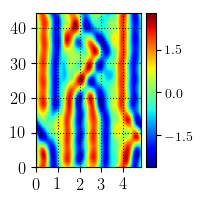
\includegraphics[width=.8\textwidth,height=.3\textheight]{MNG_ppo_tiling_init_1}
\end{minipage}
\begin{minipage}[height=.30\textheight]{.6\textwidth}
\centering \small{\texttt{(c)}}\\
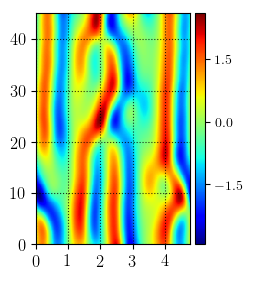
\includegraphics[width=.7\textwidth,height=.3\textheight]{MNG_ppo_tiling_final_1}
\end{minipage}
\begin{minipage}[height=.30\textheight]{.6\textwidth}
\centering \small{\texttt{(d)}}\\
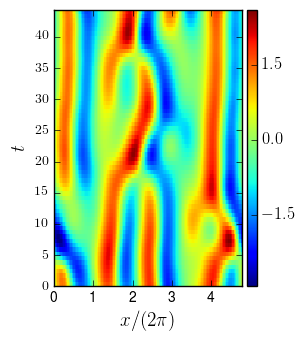
\includegraphics[width=.75\textwidth,height=.3\textheight]{MNG_ppo_L30_T44}
\end{minipage}
\caption{ \label{fig:MNG_ppotiling_one}
(a) Gluing together the three subdomains from \reffig{fig:MNG_pposubdomains_zero}
in the temporal direction. This is the initial condition for the fundamental domain
of a \twot\ with shift-reflection symmetry.
(b) The convergent result of the numerics with initial condition (a).
(c) \reffig{fig:MNG_frankenstein} \twot\
\PPOtwot{30}{44} %\emph{ppo\_L30\_T44}
included for comparison to (b).
}
\end{figure}

\begin{figure}
\begin{minipage}[height=.3\textheight]{.32\textwidth}
\centering \small{\texttt{(a)}}
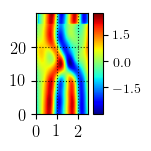
\includegraphics[width=1.0\textwidth,height=.25\textheight]{MNG_HOD_init}
\end{minipage}
\begin{minipage}[height=.3\textheight]{.32\textwidth}
\centering \small{\texttt{(b)}}
\includegraphics[width=1.0\textwidth,height=.29\textheight]{MNG_HOD_final}
\end{minipage}
\begin{minipage}[height=.3\textheight]{.32\textwidth}
\centering \small{\texttt{(c)}}
\includegraphics[width=1.0\textwidth,height=.17\textheight]{MNG_HOD_ppo_final}
\end{minipage}
\caption{ \label{fig:MNG_hod_tile}
(a) An initial condition in attempt to find the ``hook on defect tile''
used in the tilings \reffig{fig:MNG_ppotiling_zero} and
\reffig{fig:MNG_ppotiling_one}. It has been slightly modified by
including the addition of two streaks at the top of the tile, in
time.
(b) The converged \twot, its spatial shift after a prime period is close to zero, and it looks like it could be
close to a \twot, invariant under shift-reflection;
(c) The converged \PPOtwot{??}{??} fundamental domain \twot, confirmation of (b).
}
\end{figure}

After last week's plumbers union meeting I had a conversation with Michael Krygier, who works mostly
on numerical Taylor-Couette. We had a chat that inspired me to get back into investigating iterative methods
and I had an epiphany. My the truth was obscured because of the conventional computation in the literature, almost
everyone in the field that uses Newton-Krylov or other iterative methods
approximates $J^t \delta x \approx \frac{F^{t+\delta t}(x+\delta x)-F^t(x)}{|\delta x|}$. It's due to the fact that I
had seen this equation or approximation ubiquitously that I was blinded to a \emph{far} better way of performing
this computation, one that in fact \emph{I already use in the adjoint descent!}.
Namely, because the dependence on
$T$ is completely explicit in the spatiotemporal \KSe\ and doesn't rely on
implicit forward-time mappings (\ie time-integration),
all I have to do is compute the action of the matrix
$J = \frac{\partial F}{\partial x}$ on a vector $\delta x$! I can't believe
I haven't realized this until today. It's literally (up to a transpose)
how I've been employing the adjoint descent method
for many months now, but like I said the literature blinded
me I suppose.

What I mean by ``compute the action of the matrix $J$ on a vector $\delta x$''
is to decompose the matrix multiplications
into elementwise operations dependent on the spatiotemporal
Fourier mode indices. It's actually ridiculously easy and I'm just baffled
but how I didn't see it when it was right in front of my eyes.
The mathematical equation that follows is,

\beq
J\cdot x = (\ii \omegaj -q_m^2 + q_m^4 + \frac{\ii q_m S}{T})x_{n,m} + \ii q_m \mathcal{F}diag(u)\mathcal{F}^{-1}x \,.
\eeq

Such an equation can be evaluated without the use of any matrices whatsoever (the linear term with $S$ is for solutions with continuous
symmetry. There is no error or approximation (up to machine precision)
by performing the calculation in this matrix-free way (yet another boon of spatiotemporal formulation), such that the application
translates nicely to iterative methods that require the matrix-vector product, such as Newton-Krylov-Hookstep.

I messed around with a calculation but just came to the same conclusion I had previously reached, namely if the adjoint variable $v$
is chosen to be the \KSe\ then the variational derivative of the formal Lagrangian in the Ibragimov sense corresponds to the adjoint
descent direction. This is perhaps why it works so well for me. \ie the variational derivative obeys the equation

\bea
\frac{\delta L(u,v)}{\delta u} &=& -v_t + v_{xx} + v_{xxxx} - uv_x \continue
\frac{\delta L(u,-F(u))}{\delta u} &=& F_t -F_{xx} -F_{xxxx} + u F_x \equiv -J^{\dagger} F
\eea

\item[Pseudospectral spatiotemporal formulation of two dimensional Kolmogorov flow]
I believe I have derived most of the numerically relevant equations except for the specific constraints due to
discrete symmetries. Will write the ``Feynmann equation'' in pseudospectral representation, a formula for the matrix
vector product $Jx$ and a formula for the adjoint $-J^{\dagger} F$ tomorrow

\item[ETDRK4 for Jacobians]
I tried to pursue what Simon taught me in regards to calculating Jacobians when a certain numerical
integration scheme is already instantiated and known to work well. The gist of the calculation is a
lot of algebra to explicitly write the equation

\beq
\partial_t J_{n} = \frac{\partial x_{n+1}}{\partial x_n} J_n \,
\eeq

where the dependence of $x_{n+1}$ in terms of $x_n$ depends on the
underlying equations as well as the integration scheme. I haven't gotten this
to work yet likely due to the number of areas for algebra errors to occur.

I messed around with a calculation but just came to the same conclusion I had previously reached, namely if the adjoint variable $v$
is chosen to be the \KSe\ then the variational derivative of the formal Lagrangian in the Ibragimov sense corresponds to the adjoint
descent direction. This is perhaps why it works so well for me. \ie the variational derivative obeys the equation

\bea
\frac{\delta L(u,v)}{\delta u} &=& -v_t + v_{xx} + v_{xxxx} - uv_x \continue
\frac{\delta L(u,-F(u))}{\delta u} &=& F_t -F_{xx} -F_{xxxx} + u F_x \equiv -J^{\dagger} F
\eea

\item[Pseudospectral spatiotemporal formulation of two dimensional Kolmogorov flow]
I believe I have derived most of the numerically relevant equations except for the specific constraints due to
discrete symmetries. Will write the ``Feynmann equation'' in pseudospectral representation, a formula for the matrix
vector product $Jx$ and a formula for the adjoint $-J^{\dagger} F$ tomorrow

\item[ETDRK4 for Jacobians]
I tried to pursue what Simon taught me in regards to calculating Jacobians when a certain numerical
integration scheme is already instantiated and known to work well. The gist of the calculation is a
lot of algebra to explicitly write the equation

\beq
\partial_t J_{n} = \frac{\partial x_{n+1}}{\partial x_n} J_n \,
\eeq

where the dependence of $x_{n+1}$ in terms of $x_n$ depends on the
underlying equations as well as the integration scheme. I haven't gotten this
to work yet likely due to the number of areas for algebra errors to occur.

As a test of the new matrix-free GMRES code that utilizes
the matrix free exact evaluation of the matrix vector product
$J \cdot y \equiv \frac{\partial \mathbf{F}}{\partial \mathbf{x}}\cdot y$, I took
an old initial condition with a larger-than-necessary discretization. As a proof
of concept, I took the $N\times M$ discretization to be of the same order of magnitude
of the two dimensional Kolmogorov flow calculations, namely $N=M=128$. While technically
the true number of variables is halved due to the shift-reflect symmetry of the solution,
it still offered a good demonstration of why I felt this was necessary.

Starting from the same initial condition, (not utilizing adjoint descent at all)
GMRES and Gauss-Newton were run until machine precision convergence of the cost function.
Even though it only took one Newton step to converge, the time saved by GMRES is very
exciting. Specifically, the GMRES routine took 5.13613756917 seconds to converge, while Newton
took 640.616473401 seconds. In other words, the matrix free iterative method is 124.727280914
times as fast as the direct matrix-forming Newton's method. I would argue that this is
very significant and might allow the search for \twots\ on very large domains. There is
a slight cavaet, however; for numerical stability the GMRES routine does not include the spatial
domain size $L$ as a variable. Although I believe that this is not the right thing to do, I believe
there is an argument to be made as to why this is acceptable. The argument I would make is this:
towards the end of the adjoint descent procedure (when it stalls likely due to gradients becoming
small) the order of magnitude of the changes to the domain size is of order $10^{-7}$, so I believe
one should heavily favor the numerical stability in favor of minimal changes to the domain size, especially
because the solutions come in continuous families anyway.

On the other fronts, while I got preconditioned GMRES to work
the list of numerical schemes that don't seem to show nearly as much
promise include,

\begin{itemize}
\item restarted GMRES
\item BiCGSTAB
\item BFGS
\item L-BFGS
\end{itemize}

and so it isn't all good news. The main requirement for the GMRES routine
to work seems to be a relatively high dimension of the Krylov subspace, compared
to similar efforts in CFD. The solution that I tested required a maximum of about
one hundred dimensions, compared to the 8002 computational variables, which is approximately
one percent of the computational variables.

%%%%%%%%%%%%%%%%%%%%%%%%%%%%%%%%%%%%%%%%%%%%%%
\begin{enumerate}
\item To solve $J \delta x = -F(x)$, for $\delta x$, follow this procedure
\item Set $q_0 = b = -F(x)$, where $F$ is the \KSe\
\item Perform arnoldi iteration to produce orthonormal
matrix $Q_n$ that spans Krylov subspace and the upper Hessenberg matrix $H_n$
which satisfy the following relation, $JQ_n = Q_{n+1}H_n$. The shape of $Q_n$
is $dim(\mathbf{x}) \times n$ and the shape of $H_n$ is $(n+1)\times n$. (Described
in more detail below)
\item Solve nonlinear optimization problem $|| \beta e_1 - H_n y|| =0$ for $y$
\item produce GMRES correction via $\delta x = P^{-1} \cdot Q_n \cdot y$
\end{enumerate}
%%%%%%%%%%%%%%%%%%%%%%%%%%%%%%%%%%%%%%%%%%%%%%
The right preconditioned arnoldi iteration (with modified Graham-Schmidt for orthogonalization)
is written as follows in pseudo code.

for $j = 1, \cdots, m$
\bea
z_{j+1} &=& P^{-1} \cdot q_j \continue
q_{j+1} &=& J \cdot z_{j+1}
\eea
for $i = 1, \cdots j$
\bea
H_{i,j} &=& <w,q_i> \continue
q_j &=& q_j - H_{i,j}*q_i
\eea
end for
\bea
H_{i+1,i} &=& ||q_j||_2 \continue
q_j &=& q_j/||q_j||_2
\eea
end for


%%%%%%%%%%%%%%%%%%%%%%%%%%%%%%%%%%%%%%%%%%%%%%
\item[BFGS algorithm]
The Broyden-Fletcher-Goldfarb-Shanno algorithm that I attempted to implement can be written as
follows. It requires the calculation of a Hessian (of the scalar cost function)

For a quadratic model for the cost function, here designated as $f$,
\beq
m_k(p) = f_k + \nabla f_k^{\top} p + \frac{1}{2} p^{\dagger} B_k p
\eeq
the BFGS algorithm provides a minimization routine via the following,

Given $x_0, \epsilon$ and inverse Hessian $H_0$,

\begin{enumerate}
\item \textbf{While} $||\nabla f_k|| > \epsilon$
\item $p_k = -H_k \nabla f_k$
\item $x_{k+1} = x_k + \alpha_k p_k$ (Alpha given by Wolfe curvature conditions, will describe below)
\item $s_k = x_{k+1} - x_k$
\item $y_k = \nabla f_{k+1} - \nabla f_{k}$
\item $z_k = \frac{1}{y_k^{top}s_k}$
\item $H_k = (\mathbb{I}-z_k s_k y_k^{\top})H_k(\mathbb{I}-z_k y_k s_k^{\top}) + z_k s_k s_k^{\top}$
\end{enumerate}

The Wolfe conditions that determine the ``step size'' $alpha_k$ are given by the following,
find $alpha_k$ such that the following hold,

\bea
f(x_k + \alpha_k p_k) &\leq& f(x_k) + c_1 \alpha_k \nabla f_k^{\top} p_k \continue
\nabla f(x_k + \alpha_k p_k)^{\top} p_k &\geq& c_2 \nabla f_k^{\top} p_k
\eea
%%%%%%%%%%%%%%%%%%%%%%%%%%%%%%%%%%%%%%%%%%%%%%%%%%%%%%%%%%%%%%%
\begin{enumerate}
\item $r_+ = s_i (\alpha_i - \beta)$
\item end for
\item $p_k = -r$
\item $x_{k+1} = x_k + \alpha_k + p_k$ (alpha from wolfe conditions)
\item if $k>m$
\item Discard $(s_{k-m},y_{k-m})$
\item end if
\item $s_k = x_{k+1} - x_k$
\item $y_k = \nabla f_{k+1} - \nabla f_k$
\item $p_k = -H_k \nabla f_k$
\item $x_{k+1} = x_k + \alpha_k p_k$ (Alpha given by Wolfe curvature conditions, will describe below)
\item $s_k = x_{k+1} - x_k$
\item $y_k = \nabla f_{k+1} - \nabla f_{k}$
\item $z_k = \frac{1}{y_k^{top}s_k}$
\item $H_k = (\mathbb{I}-z_k s_k y_k^{\top})H_k(\mathbb{I}-z_k y_k s_k^{\top}) + z_k s_k s_k^{\top}$
\end{enumerate}


\item[L-BFGS algorithm]
The following is an adaptation of the BFGS algorithm that makes it possible to optimize the
same quadratic model without holding full matrices in memory.

\begin{enumerate}
\item Let $m$ be the maximum number of column vectors to hold in memory
\item \textbf{While} residual $>$ tolerance and $k<$ maximum step number
\item $q = \nabla f_k$
\item If $k>m$,
\item for $i = k-1 ,\cdots , k-m$
\item $z_i = \frac{1}{y_i^{\top} s_i}$
\item $a_i = z_i s_i q$
\item $q = q - a_i*y_i$
\item end for
\item $r = H_k^{0}q$
\item for $k-m-1,\cdots, k-1$
\item $\beta = z_i y_i^{\top} r$
\item $r_+ = s_i (\alpha_i - \beta)$
\item end for
\item $p_k = -r$
\item $x_{k+1} = x_k + \alpha_k + p_k$ (alpha from wolfe conditions)
\item if $k>m$
\item Discard $(s_{k-m},y_{k-m})$
\item end if
\item $s_k = x_{k+1} - x_k$
\item $y_k = \nabla f_{k+1} - \nabla f_k$
\item $p_k = -H_k \nabla f_k$
\item $x_{k+1} = x_k + \alpha_k p_k$ (Alpha given by Wolfe curvature conditions, will describe below)
\item $s_k = x_{k+1} - x_k$
\item $y_k = \nabla f_{k+1} - \nabla f_{k}$
\item $z_k = \frac{1}{y_k^{top}s_k}$
\item $H_k = (\mathbb{I}-z_k s_k y_k^{\top})H_k(\mathbb{I}-z_k y_k s_k^{\top}) + z_k s_k s_k^{\top}$
\end{enumerate}

\item[BiCGSTAB algorithm]
Just to include this as a final algorithm,

Given $r_0= b - Ax_0, \alpha_0 = \rho_0 = w_0 =p_0 = 1$
\begin{enumerate}
\item \textbf{While} residual $>$ tolerance
\item For $i = 1, \cdots , $
\item $\rho_i = <r_0, r_i>$
\item $\beta = \frac{\rho_i}{\rho_{i-1}} \frac{\alpha_i}{w_i}$
\item $u = r_i + \beta q_i$
\item $p_i = u + beta(q_i +beta*p_i)$
\item $y = P^{-1}p_i$
\item $v = J y$
\item $\alpha = \rho_i / <r_0,v>$
\item $q_i = u - alpha v$
\item $z = P^{-1}(u+q_i)$
\item $x_{i+1} = x_i + alpha * z$
\item If $x_{i+1}$ satifies tolerance, exit, else
\item $r_{i+1} = r_i - \alpha J z$
\end{enumerate}


\item[Pseudospectral spatiotemporal formulation of 2-D Kolmogorov flow]
The equations governing two dimensional Kolmogorov flow can be written in terms
of velocity field $\mathbf{u}$(eliminated later) and vorticity $\omega$ in the
following manner. For now I will just write the homogeneous equations, with
forcing easily added afterwards

\beq
\omega_t - \hat{z}\cdot(\nabla \times (\mathbf{u}\times \omega \hat{z})) - \frac{1}{Re}\nabla^2 \omega = 0
\eeq

The only difficult part of rewriting this equation in terms of $(2+1)$ spatiotemporal Fourier coefficients
(assuming periodic boundary conditions) is the nonlinear term, not only due to the cross products
but the necessity to express the velocity field in terms of the streamfunction, and consequently the
vorticity field as $\mathbf{u} = \nabla \times (\nabla^{-2} \omega)$
which is possible due to the two dimensional approximation. The operator $\nabla^{-2}$ is the inverse
of the Laplacian, which is technically singular; I asked around and the standard practice is to essentially
define it in fourier space as $\frac{1}{|\mathbf{k}|^2}$, where $|\mathbf{k}|^2 = k_x^2 + k_y^2$. For
numerical purposes its apparently common practice to say that the inverse of the $k_x = k_y = 0 $
term equals $1$. In other words, $1/0 = 1$. It's just a means of approximating the operator in
spectral space.

Although \refref{ChaKer12} give nice formula that is almost entirely of Fourier coefficients, I find it
more useful to completely eliminate the velocity field components $\mathbf{u} = (u,v)$ from the equation.

Therefore, the pseudospectral (homogeneous) spatiotemporal equation takes the form,

\bea \label{eqn:2DK_spectral}
\ii \omega \Omega &+& \ii k_x \mathcal{F}[\mathcal{F}^{-1}(\frac{\ii k_y}{|\mathbf{k}|^2} \Omega)* \mathcal{F}^{-1}(\Omega)] \continue
                  &-& \ii k_y \mathcal{F}[\mathcal{F}^{-1}(\frac{\ii k_x}{|\mathbf{k}|^2} \Omega)*\mathcal{F}^{-1}(\Omega)] \continue
                  &-& \frac{|\mathbf{k}|^2}{Re} \Omega = G(\Omega,T,L_x,L_y) = 0
\eea

Likewise, if allowed to write differentiation operators via $D_t,D_x,D_y$, etc, then the jacobian
takes on the form in pseudospectral representation,

\bea \label{eqn:2DK_spectral_jac}
J   &=& D_t + D_x \mathcal{F}[diag(D_y \nabla^{-2} \omega)\mathcal{F}^{-1} + diag(\omega)D_y \nabla^{-2}\mathcal{F}^{-1}]\continue
    &-& D_y \mathcal{F}[diag(D_x \nabla^{-2} \omega)\mathcal{F}^{-1} + diag(\omega)D_x \nabla^{-2}\mathcal{F}^{-1}] \continue
    &-& \frac{\nabla^2}{Re}
\eea

By taking the complex conjugate and multiplying by the Feynman equation \refeq{eqn:2DK_spectral},
the expression for the adjoint descent direction, $-J^{\dagger}G$.

\bea \label{eqn:2DK_adjointdescent}
-J^{\dagger}G  &=& [D_t + \mathcal{F}diag(D_y \nabla^{-2} \omega)\mathcal{F}^{-1} D_x \continue
               &-& \mathcal{F} \nabla^{-2} D_y diag(\omega)\mathcal{F}^{-1}D_x \continue
               &-& \mathcal{F}diag(D_x \nabla^{-2}\omega)\mathcal{F}^{-1} D_y\continue
               &+& \mathcal{F} \nabla^{-2} D_x diag(\omega)\mathcal{F}^{-1}D_y \continue
               &-& \frac{\nabla^2}{Re}] \cdot G
\eea


\item[Jacobian integration from ETDRK4 scheme]
The Exponential time differencing in conjunction with Runge-Kutta 4th order\rf{ks05com} as
an integration scheme for stiff equations has used by many people to integrate the \KSe.
I recall sifting through the Kuramoto-Sivashinsky literature and almost everyone used this integrator,
due to its ability to handle the stiffness of the linear term and explicitly evaluate the nonlinear term.

Something that I never saw, however, was a calculation that directly follows, which is taking the
derivative of the time integration scheme itself to provide a reliable integration scheme
for Jacobian's. I recall in Ruslan's codes he uses some sort of interpolation to produce
the Jacobian but I think maybe Burak has already done this. I can't say for certain because I haven't been
through all of the codes in the repository.

Regardless, the ETDRK4 scheme evaluates the stiff, linear portion of the \KSe\ via what are
essentially integrating factors, and then calculate the nonlinear terms accordingly.

Given $v$, a set of spatial Fourier coefficients, the scheme can be written
relatively succinctly via the use of a number of constant operators in the problem
which are created by various numerical combinations of the exponentiated linear operator
of the \KSe. I'll leave the details to the reader in \refref{ks05com}, but for any given
discrete time step, we can write, (using $n$ as a discrete time subscript)

\bea
N(v_n) &=& \frac{-\ii \mathbf{q}}{2}\mathcal{F}((\mathcal{F}^{-1}(v_n))^2) \continue
a_n &=& E_2*v_n + Q*N(v_n)\continue
N(a_n) &=& \frac{-\ii \mathbf{q}}{2}\mathcal{F}((\mathcal{F}^{-1}(a_n))^2)\continue
b_n &=& E_2*v_n + Q*N(a_n)\continue
N(b_n) &=& \frac{-\ii \mathbf{q}}{2}\mathcal{F}((\mathcal{F}^{-1}(b_n))^2)\continue
c_n &=& E_2*v_n + Q*(2*N(b_n)-N(v_n)\continue
N(c_n) &=& \frac{-\ii \mathbf{q}}{2}\mathcal{F}((\mathcal{F}^{-1}(c_n))^2)\continue
v_{n+1} &=& E*v_n + f_1*N(v_n) + 2f_2*(N(a_n)+N(b_n))+f_3 N(c)
\eea

Now, we can take the derivative of the last equation for $v_{n+1}$ with respect to $v_n$,
to get the velocity gradient matrix, $A(v_n) \equiv \frac{\partial v_{n+1}}{\partial v_n}$

The derivatives of each of the nonlinear functions looks like the following via the chain rule
\bea
\frac{\partial N(x_n)}{\partial v_n} &=& (-\ii \mathbf{q} \mathcal{F} \continue
                                     &*&(diag(\mathcal{F}^{-1}(x_n))\mathcal{F}^{-1}))*\frac{\partial x_n}{\partial v_n}
\eea

Because of the nested nature of the Runge-Kutta integration scheme, a pattern quickly emerges such
that it becomes smart to define the following, let the velocity gradients matrix evaluated at
each variable, $a_n,b_n,c_n,v_n$ be represented by $A_v, A_a, A_b, A_c$. With this and the
following substitutions,
\bea
\tilde{A}_v &=& (E_2 + Q A_v) \continue
\tilde{A}_a &=& A_a(E_2 + Q A_v) \continue
\tilde{A}_b &=& A_b(E_2 + Q \tilde{A}_a) \,,
\eea

it becomes much easier to write an explicit expression for the desired quantity,

\beq
A(x_n) = \frac{\partial v_{n+1}}{\partial v_n} = E + f_1 A_v + 2 f_2[\tilde{A}_a + \tilde{A}_b] \\
+ f_3 A_c[ E_2 \tilde{A}_v + 2Q\tilde{A}_b - Q A_v]
\eeq

I believe that this equation, in accordance with the equation
\beq
\dot{J} = AJ
\eeq

should yield an accurate integration scheme for finding Jacobian's and hence stability multipliers
or exponents for periodic orbits.


Trying to put the finishing touches on the written document for my thesis proposal.
While sourcing some of my written statements I stumbled across something interesting
in \refref{witt99hol}, displayed in the quote,

\begin{quote}
We believe that the longer time scales for the excited modes arise from the metastability
of the cellular solutions (which are stable for small L) undergoing continuous creation
and annihilation events (``space-time defects'')\rf{ChowHwa95}
\end{quote}

It is \refref{ChowHwa95} that is the earliest reference to ``space-time defects'' that I have
found. The lion's share of the work presented is regarding wavelet-based simulation
as well as statistical computations but there are certain ideas that could possibly
be useful for my needs.

Both of these papers discuss spatial and temporal scales as well as reframe
dynamics in terms of ``metastable cellular solutions'', ``space-time defects'' and
in \refref{ChowHwa95} they reference the system (\KSe) being ``frustrated'' by the existence
of multiple ``metastable cellular states''.

I haven't delved too deep into either paper but on the surface it seems like there
is some low-hanging fruit that can be picked for spatiotemporal purposes.

\begin{figure}
\begin{minipage}[height=.3\textheight]{.32\textwidth}
\centering \small{\texttt{(a)}}
\includegraphics[width=1.0\textwidth,height=.25\textheight]{MNG_HOD_init}
\end{minipage}
\begin{minipage}[height=.3\textheight]{.32\textwidth}
\centering \small{\texttt{(b)}}
\includegraphics[width=1.0\textwidth,height=.29\textheight]{MNG_HOD_STREAK_init}
\end{minipage}
\begin{minipage}[height=.3\textheight]{.32\textwidth}
\centering \small{\texttt{(c)}}
\includegraphics[width=1.0\textwidth,height=.17\textheight]{MNG_HOD_STREAK_final}
\end{minipage}
\caption{ \label{fig:MNGhodstreak}
(a) Initial condition from \reffig{fig:MNG_HOD_tile} that converges to
a solution that is believed to be a numerical continuation of (b) from \reffig{fig:MNGsymb11}. (b) An initial condition
resulting from concatenating a streak-pair with (a), that
numerically converges to (c).
}
\end{figure}

\begin{figure}
\begin{minipage}[height=.3\textheight]{.32\textwidth}
\centering \small{\texttt{(a)}}
\includegraphics[width=1.0\textwidth,height=.25\textheight]{MNG_HD_init}
\end{minipage}
\begin{minipage}[height=.3\textheight]{.32\textwidth}
\centering \small{\texttt{(b)}}
\includegraphics[width=1.0\textwidth,height=.29\textheight]{MNG_HD_STREAK_final}
\end{minipage}
\begin{minipage}[height=.3\textheight]{.32\textwidth}
\centering \small{\texttt{(c)}}
\includegraphics[width=1.0\textwidth,height=.17\textheight]{MNG_HD_STREAK_final}
\end{minipage}
\caption{ \label{fig:MNGhdstreak}
(a) Initial condition that has not been shown to numerically converge. (b) An initial condition
resulting from concatenating a streak-pair with (a), that
numerically converges to (c).
}
\end{figure}


I've been reading the Least Squares Shadowing method developed in \rf{Wang14}
and mentioned in both \rf{LaShMe18,Lasagna17}. I had a former roommate explain
adjoint methods and their application in an engineering context. Typically from
what I have seen in adjoint methods is that engineers acknowledge that solving
for the full velocity field is hard so they write the adjoint equations such
that there are only a few control variables being varied instead of a very high
dimensional flow field. I believe this is because engineers are predominately
searching for stable equilibria by varying control parameters such as: airfoil
geometry, drag coefficient, etc.

I think I need to read the Lasagna papers more thoroughly to see how the LSS
method is applied to chaotic systems. I believe Wang's method only applies for
finding the derivatives of observables w.r.t scalar control variables, in my
case this would be the domain size, period, spatial shift (or energy, or another
conserved quantity yet to be discovered).

Trying to get back into the swing of things by pursuing Lan's method
of plotting partial derivatives in order to develop some intuition regarding the admissible
spatial and temporal combinations of tiles in order to develop the symbolic dynamics.

I don't have anything worth showing really but I'm starting to believe that the spatial
itineraries might be decoupled from the temporal ones; I haven't really developed
an idea as to what is the best way to plot these yet, but following \rf{DoLa14}
and plotting in the $u,u_x$ plane and taking temporal cross sections of \spt\ \twots\
shows patterns similar to spatial equilibria ($T=0$ system). I believe this makes
sense as spatially conjoining two tiles means that each time instance must be periodic in space;
therefore I believe the intuition is something like follows: To glue two tiles $0$,$1$ spatially,
then at each instant in time the combination needs to be topologically equivalent to a spatial
equilibrium $01$. This is really hard to demonstrate other than rather vague attempts such
as the time dependent trajectory in $(u,u_x,u_t)$ space needs to intersect $(u,u_x,0)$ plane
to be able to glue spatially; this always seems to be the case so I believe a first
trial would be to continuously attempt to glue \eqva\ to an orbit and see if it can
be repeated ad nauseam. This could be misguided due to unwarranted projections, but
currently plotting trajectories as functions of space and time is far too obfuscating
to be useful. (similar to plotting trajectories prior to quotienting continuous symmetry
or plotting Fourier coefficients).

I believe this best way to proceed is to tile repetitively in space or time and then analyze the
corresponding partial derivative plots.

My intentions for future edits of the paper; general
additions like including figures and citations are left out
in favor of more explicit goals.

Others would know better than me, but my gut is telling me that
if the paper is titled ``Spatiotemporal tiling of the \KS\ flow''
then incorporating Gutkin and Osipov is consistent with this message.
I foresee this process unfolding in two ways:
1. The paper is aimed at the overarching topic of spatiotemporal tiling,
for example, ``Spatiotemporal tiling of both discrete and continuous nonlinear
dynamical systems'' and the computational details such as adjoint method, GMRES,
etc. are left to another, more technical, paper.
2. The focus of the paper is the \KSe\ and the methods with which new solutions
have been found and can be constructed. This would go over the specific numerical
methods for finding solutions as well as gluing and tiling. I don't think \spt\
cats fits into this message personally.

For the second option I propose the following outline for the paper

\begin{enumerate}
\item Abstract
\item Intro
\item \KSe\ literature review
\item \Spt\ \KSe\ in Fourier basis (\texttt{sFb.tex})
\item \Spt\ symmetries
\item \Spt\ symbolic dynamics concept
\item Descent methods
\item Iterative methods
\item Gluing methods
\item Tiling methods
\item (If possible) symbolic dynamics quantitatively explained
\item Conclusion
\end{enumerate}
with the following reserved for appendices of either the paper or
thesis
\begin{itemize}
\item Variational methods
\item Matrix-free computations
\item Preconditioning
\item Fourier transform conventions and selection rules
\end{itemize}
with the caveat that if the Ibragimov-type study pans out, then
the results would be moved to the variational methods section which
would in turn be inserted between symbolic dynamics concepts and
descent methods. This is the narrative that I believe has the most
continuity. There is not much application of discrete Lagrangian methods
similar to \refref{KraMaj15}. While I believe this work is formulated
as a variational problem, almost all of the key components of discrete Lagrangian
methods are missing. For example, we do not formulate discrete jet bundles, discrete
action principles, discrete Noether's theorem, etc. These results are inherently
different from our calculation because they work in a discretized configuration
space $(x,t)$ and define everything in terms of finite differences on these
grid points.

The second option is more akin to how I believe my thesis will be structured
and so I am biased to approve of this format more. Due to the already
exorbitant length of \texttt{GuBuCv17.tex} I think that actually there
should be three papers: A \spt\ cat paper, a \spt\ \KS\ paper, and a
``grand narrative'' paper which builds on the results of the first two.



After some thought I realized that the
method I was using to produce the initial
conditions for the gluing procedure was
a terrible idea and the truncation of the
Fourier modes was much better than the use
of convex combinations and Fourier truncation.

The reason for this is that although the smoothing
of the piecewise linear functions would result in
a continuous field that would like the constituent
\twots\ together the tangent space would be terribly
wrong. I attribute the success of the gluing in spite
of this to the potency of the \spt\ numerical methods (adjoint
descent, etc.)

I will propose an improvement (whose implementation
I will reserve for after the paper is written due to
the amount of work involved).

The method by which I believe that solutions should be
glued, or at least the initial \twots\ should be
joined is to solve a supplementary problem which
fills in a zero padded region by virtue of approximately
solving the BVP problem induced by the connection of the boundaries
of each \twot.

Specifically, because we are more concerned with the
tangent space being correct we will utilize Neumann
boundary conditions for the BVP. Because of these
boundary conditions the ``natural'' choice for the
discretization of this connecting region is to
either used finite difference methods or
Chebyshev collocation methods. The former
is rather expedient and perhaps would be better
for this additional optimization problem because
it will not result in an exact solution either way.

The reason we know that the intermediate area
cannot have a tangent space that satisfies the \KSe\
everywhere locally is because we are connecting two
\twot\ solutions. For instance, integration of the
IVP initiated at either boundary would (theoretically)
result in the \twot\ being repeated ad infinitum.

There is still indecision on my part as to the
precise method by which the problem could be solved.

The first, a fully \spt\ method, would allow for
use of the currently implemented (with modifications
to incorporate the boundary conditions) numerical
methods. The idea is to merely follow the typical
procedure except the basis would be either Fourier-Chebyshev
or Chebyshev-Fourier depending on the gluing direction.

The second (more straightforward in my mind) method
would be to apply the variational Newton descent formalism
to a Chebyshev basis with Neumann BC. This would be
easily accomplished by using a Chebyshev basis and
differentiation operator instead of the finite difference
methods. The only difference between the spatial gluing
and temporal gluing cases would then be
the tangent space equations,
namely, whether we are using \refeq{e-Fks} or \refeq{e-ksX}
in the variational Newton descent equation.

As I'm writing this I don't think the \spt\ method would
really be that difficult. The only difference from the
current \spt\ method would be to incorporate Chebyshev
transforms and modify the differential
operators to accomodate the boundary conditions.
For instance, if tackling Neumann BC
in time then for an $N$ by $M$ time by space discretization
(Fourier in space, Chebyshev in time) then the
correct form of the equation would take the spectral
coeff
Let $u_t(A)$ and $u_t(B)$ represent the first time
derivative evaluated on the ``boundary'' of each solution.
In matrix notation we have the following
<<<<<<< .mine

Fluid flows are well described by the Navier-Stokes equation. Instead of
beginning research with a partial differential equation with three
spatial dimensions, it is wiser to begin with simpler partial
differential equation, e.g. ``Navier-Stokes'' in one spatial dimension,
in order to gain some intuition about the larger picture.


One of the simplest partial differential equations that exhibits
spatiotemporal chaotic behavior is the \KS\ [henceforth KS]
system\rf{KurTsu76,siv}, which is used to model a number of different
phenomena, such as unstable flame fronts. The equation for the velocity
of such a flame front
$u(\conf, \zeit)$ on a periodic domain, $u(\conf, \zeit)= u(\conf + L,
\zeit)$.
\beq
    u_\zeit + \frac{1}{2}(u^2)_\conf + u_{\conf \conf} + \nu u_{\conf \conf \conf \conf} = 0 \, \quad x \in [0, L]
\eeq
The terms each contribute differently to the dynamics: $u_{\conf \conf}$
contributes to instability, $u_{\conf \conf \conf \conf}$ provides
damping, and $u^2_{\conf}$ transfers energy between large and small
scales (e.g. between Fourier modes with small and large wavenumbers).

The equations can be made dimensionless by scaling out the 'viscosity'
$\nu$ with transformations $\conf \rightarrow \conf\nu^{1/2}, \zeit
\rightarrow \zeit\nu , u \rightarrow u\nu^{-1/2}$. Hence the
\KSe\ takes the non-dimensionalized form:
\beq
     u_\zeit + \frac{1}{2}(u^2)_\conf + u_{\conf \conf}
     + u_{\conf \conf \conf \conf} = 0 \, \quad x \in [0, L\nu^{-1/2}]=[0,2\pi\tildeL]
\ee{ks}
In these dimensionless units, periods of periodic solutions are also
rescaled following the relation: $T_p = \frac{T^{*}_p}{\nu}$.

Possible avenues of study of the equation and its behavior include
varying $L$ while keeping $\nu = 1$, or varying $\nu$ while keeping $L =
1$ or $2\pi$.

The \KS\ equation have a number of different symmetries, namely: spatial
translational invariance, temporal translation invariance, reflection
invariance, and Galilean invariance. In order to exploit the periodicity
of the equations, we recast the field in its Fourier representation
\beq
u(\conf, \zeit) =
\sum_{k = -\infty}^{\infty} \Fu_k e^{iq_kx} \quad \mbox{where } \, q_k = \frac{2\pi}{L}
\,.
\eeq
The \KSe's representation in terms of spatial Fourier modes is then:
\beq
\dot{\tilde{u}}_k = (q_k^2-q_k^4)\Fu_k-i\frac{q_k}{2}\sum_{m=-\infty}^{\infty}\Fu_m\Fu_{k-m}
\,.
\eeq
The hyper-viscosity term $-q^{4}_k$ term, damps the higher modes such
that a truncation of Fourier modes still yields accurate results, however
different numbers of modes can inherently change the nature of the
solution in the asymptotic limit.

One can also look at the antisymmetric subspace of the full \statesp\
defined by $u(\conf,\zeit)=-u(-\conf,\zeit) \in \bbU^+$. The subspace
$\bbU^+$ can be described with the case of purely imaginary Fourier
coefficients $\Fu_k \rightarrow i\Fu_k$, such that the evolution equation
becomes:
\beq
\dot{\tilde{u}}_k
= (q_k^2-q_k^4)\Fu_k-\frac{q_k}{2}\sum_{m=-\infty}^{\infty}\Fu_m\Fu_{k-m}
\,.
\eeq
By doing so, one eliminates the continuous translational symmetry that is
present in the full \statesp\ formulation.


There are plenty of ways to visualize the evolution of solutions to the
\KSe, however not all visualizations are equal in terms of insight or
usefulness. In our applications, pretty plots of the spatiotemporal
dynamics of $u(\conf, \zeit)$ are usually not the most useful for further
analysis; projections of trajectories in $\infty$\dmn\ \statesp s are often
more useful.
Furthermore, Poincar\'e return maps often offer more information than the
full \statesp\ pictures, specifically about the fractal structure of
strange attractors.


By setting $u_t = 0$ and integrating over \refeq{ks} once, one arrives at
\beq
\frac{1}{2}u^2 + u_\conf + u_{\conf \conf \conf} = c
\,,
\eeq
which we can write as $3$ ODEs in $\conf$,
\beq
u_\conf = v ,\quad v_\conf = w , \quad w_\conf = u^2 - v -c
\,.
\eeq
This equation exhibits a reversal symmetry, $\conf \rightarrow
-\conf , u \rightarrow -u , v \rightarrow v , w \rightarrow -w$.
The third equation can be rewritten as
\beq
(u+w)_x = u^2 - c
\,.
\eeq
For us the interesting dynamics occurs for $c>0$. The sets of bounded
solutions are complex and fractal in nature. The equilibria in this
regime are given by $c_+ = (\sqrt{c},0,0)$ and $c_- = (-\sqrt{c},0,0)$.
One can acquire the Floquet multipliers by linearizing the flow around
one of the equilibria; the opposite equilibria will exhibit a reversed
stability profile due to the 'time' reversal symmetry previously
mentioned.

For fixed system size $L$, the only surviving equilibria have periodicity
equal to $L$. The corresponding equilibrium condition is then:
\beq
q^2_k (1-q^2_k)\Fu_k + i\frac{q_k}{2}\sum_{m=-\infty}^{\infty}\Fu_m \Fu_{k-m} = 0
\,.
\eeq
On a finite periodic domain, the spatially periodic equilibria have periods which
are multiples of $L$. There is a bifurcation every time $\tildeL$
crosses and integer value, i.e. when $\tildeL = n$, $n$-cell states are
generated through pitchfork bifurcations.
    %\PC{2016-08-15}{\tildeL\ has not been defined anywhere}

In the full \statesp\ they form an invariant circle due to translational
invariance.

In the antisymmetric subspace $\bbU^+$ the aforementioned equilibria
correspond to two points, which are half-period translations of each
other:
            %\PC{2016-08-08}{you have not yet defined `the antisymmetric
            %subspace', this remark cannot be understood here..}
\beq
\nonumber
u(\conf, \zeit) = -2\sum_k \Fu_{kn}\sin{(kn\conf)} \quad \mbox{where,} \quad \Fu_{kn} \in \mathbb{R}
\eeq
The spatially periodic solutions is finite, due to the finite allowance
of zeros of analytic functions on a finite-dimensional compact manifold.


The time-evolution stability matrix evaluated at an \eqv\ $\ssp_q$ is
constant, therefore the Jacobian follows by exponentiation:
\beq
\nonumber
\J^{t}\,(\ssp_q) = e^{At} \quad \mbox{where,} \quad A = A(\ssp_q)
\,.
\eeq
For small $\tildeL<1$, $u(\conf, \zeit) = 0$ is a globally attractive
stable equilibrium. As $\tildeL$ increases, there is a sequence of
bifurcations that affects the dynamics in an unstable and `turbulent'
manner.

Long wavelength perturbations are linearly unstable, while short
wavelength perturbations are strongly contractive. For example, an
equilibrium solution can be very unstable in 5 eigen-directions, but with
strong contraction in higher, stable eigen-directions. In particular, the
equilibrium $u(\conf,\zeit)=0$ has Fourier modes as linear stability
eigenvectors. The Fourier modes who satisfy $|k|<\tildeL$ are unstable.
The most unstable mode has $k$ closest to $\frac{\tildeL}{\sqrt{2}}$.

Truncation of higher Fourier modes can by justified through the following
analysis: If the initial $\Fu_k$ are small then the bilinear term $\Fu_m
\Fu_{k-m}$ can be neglected. Then the equations become decoupled linear
equations whose solutions are exponentials. There are then a finite
number of modes growing with time. These unstable modes excite the higher
modes through the bilinear term. However, higher modes are highly damped.
Therefore the intermediate wavelengths play an important role in
maintaining a dynamic, on-average equilibrium, but truncation can be
employed so long as all important modes are kept. A consequence of this
is that an infinite-dimensional problem has become finite dimensional.

There is no chance of reversing the evolution because of the high (in
principle infinite) number of highly-contracting modes. The time reversal
turns these into highly unstable modes.

\Eqva\ are important because they play two different roles:
\begin{itemize}
\item More unstable directions implies less time spent by an orbit in its neighborhood.
\item Orbits spend large fractions of time in neighborhoods of equilibria with only a few unstable directions.
\end{itemize}

The best coordinate system to use are generated by the
stable/unstable manifolds. It would be best to find a coordinate
 transformation to new, curvilinear coordinates where the dynamics
  take place but it's not known if this can be done, let alone if it can be done globally.



The space average of a function $a(\conf, \zeit)$ periodic on the interval $L$ is given by
\beq
\left<a\right> = \left<a\right>(\zeit) = \frac{1}{L}\oint a(\conf,\zeit)\,dx
\eeq
Total derivatives vanish via spatial periodicity, and integration by parts yields
\beq \nonumber
\left<f_x\right> = 0, \quad \left<f_xg\right> = -\left<fg_x\right>
\eeq
The mean value of time dependent $\left<a\right>(\zeit)$ is given by
\beq
\bar{a} = \lim_{t\to\infty}\frac{1}{t}\int_{0}^{t}\,d\tau \,\left<a\right>
\eeq
The average value of a function on a periodic orbit only requires the
integration over one period. For an equilibrium the time
average is equal to the space average, which is in turn equal to the
value of the function evaluated at the equilibrium.

For the \KSe\ the local velocity square, ${u^2}/{2}$, can be interpreted
as the kinetic energy density when used in the spatial average equation.

Because the Fourier modes are eigenvectors of the translation operator,
the energy is a diagonalized quadratic norm in Fourier space.
\beq
E = \sum_{k=1}^{\infty} E_k , \quad E_k = \frac{1}{2}|a_k|^2
\eeq
By applying a time derivative, a substitution of variables and
integration by parts, one arrives at
\beq
\dot{E} = P - D , \quad P = \left<u^2_x\right>, \quad D = \left<u^2_{xx}\right>
\eeq
As the time averaged energy density on a generic orbit is expected to go
to a constant, on average the power-in $P$ and the dissipation rate$D$
balance each other.

In the Fourier basis the conservation of energy can be written
\beq
\sum_{k=-\infty}^{\infty}\,(q^2_k-q^4_k)\overline{E}_k
\eeq
Therefore $\overline{E}_k$ have to decrease faster than $q^{-4}_k$.

There are three main methods by which one can attempt to integrate a PDE:
\begin{itemize}
\item Discretize the configuration space by means of a grid of $N$ points
    and approximate the derivatives $u_\conf$, $u_{\conf \conf}$, and
    $u_{\conf \conf \conf \conf}$ with a finite difference scheme of
    appropriate order.
\item Integrate the equations for a finite number of (truncated) Fourier
    modes, paying attention to the stability of the integrator and
    stiffness of the equations.
\item Pseudo-spectral integration of the equations: at each step calculate
    the nonlinear term in configuration space and then bring
    the result back to Fourier space.
            %\PC{2016-08-08}{I thought you compute the nonlinear term in the
            %configuration space, then Fourier transform it?}

\end{itemize}



In this report I will describe my efforts towards implementing MATLAB
code that allows for spatial integration of the \KSe. The big caveat is
that I have still not been able to accomplish this, at least as of the
time of the current version of this report.


The one spatial dimension \KSe\ is given by
\beq
    u_\zeit + u u_\conf
    + u_{\conf \conf}+\nu u_{\conf \conf \conf \conf} = 0 \,,
    \label{e-MNGre1}
\eeq
The terms of this equation all play different roles: $u_{\conf \conf}$
is an ``anti-diffusion'' term, that pumps energy into the system and
feeds instabilities on large length scales,
$u_{\conf \conf \conf \conf}$ which provides damping on small  length scales, and
the nonlinear, inertial term $u u_\conf$ which transfers energy between
large and small scales. The ``hyper-viscosity" $\nu$ plays through
the dimensionless parameter $\tildeL = L/(2\pi \sqrt{\nu})$ a role analogous
to the role that the Reynolds number $Re$ plays in the Navier-Stokes equation.

When the \KSe\ is taken with spatially periodic boundary conditions
$u(\conf + L, \zeit) = u(\conf, \zeit)$,  $u(\conf, \zeit)$
can be interpreted as  the vertical velocity
field of a ``ring of fire'', produced by a Bunsen burner, for example. A
number of studies\rf{kstroy89,kstroy92,ksgreene88,Mks86,DoLa14}
explore the steady solutions of this system, i.e., where $u_t = 0$.
These solutions are important when viewed from a topological perspective,
as the equilibria play a role in the organization of the \statesp.


In order to get into spatial integration of a time-strip, one must first generate the time strip. Because of the spatial periodicity of $u(\conf, \zeit)$, the time evolution of solutions is best done in Fourier space. The \KSe\ in Fourier space takes the form,

\beq
\dot{\tilde{u}}_k = (q_k^2-q_k^4)\Fu_k-i\frac{q_k}{2}\sum_{m=-\infty}^{\infty}\Fu_m\Fu_{k-m}
\label{e-MNGre2}
\eeq

The term with $-q_k^4$ serves to damp higher Fourier modes, which allows accurate and stable results even when truncating the infinite number of Fourier modes, a notion that makes numerical implementation feasible. Also, because $u(x,t)$ is a physical and hence, a real quantity, there also exists the relation between Fourier coefficients $u_{-k}=u_k^{*}$. Therefore for a truncation that keeps $N$ Fourier modes, we can rewrite the Fourier space equation as,

\beq
\dot{\tilde{u}}_k = (q_k^2-q_k^4)\Fu_k-i\frac{q_k}{2}\sum_{m=0}^{N/2-1}\Fu_m\Fu_{k-m}
\label{e-MNGre3}
\eeq

To integrate this equation numerically, we first start with spatially
discretizing the \KS\ system by Fourier expanding the field
$u(\conf_n,\zeit)= u_n(\zeit)$ over $N$ points of a periodic spatial
lattice $\conf_n = n L/N$,
\bea
  \Fu_k(\zeit) &=& \frac{1}{N} \sum^{N-1}_0 u_n(\zeit) e^{-iq_k\conf_n}
  \,=\, \frac{1}{N} \sum^{N-1}_0 u_n(\zeit) e^{-i 2 \pi k n /N}
  \,,\quad
q_k = \frac{2 \pi k}{L}
\continue
  u_n(\zeit) &=&\sum_{k=-N/2+1}^{N/2}\Fu_k(\zeit) e^{iq_k\conf_n}
    \,=\, \sum_{k=-N/2+1}^{N/2}\Fu_k(\zeit) e^{i 2 \pi k n /N}
\,,
\label{e-MNGre4}
\eea

where $k$ ranges from $-N/2+1$ to $N/2$ due to how MATLAB's Fast
Fourier Transform (FFT) handles an even number of configuration space points.
 In order to have a completely symmetric spectrum, one would need to have an
 odd number of configuration space points, which depending on the number and
  size of prime factors, would increase the computation time.

Following in the footsteps of others, MATLAB code \texttt{kursiv.m}
originating from Kassam and Trefethen\rf{ks05com}, is adapted in order
to provide accurate time-evolution data of $u_n(\zeit)$. The scheme used
 in this implementation is a combination of two different methods,
 Exponential Time Differencing (ETD) and Fourth Order Runge-Kutta (RK4)
 to form a new schema aptly abbreviated ETDRK4. All of this is applied in
 \texttt{ksint.m} which was written by Xiong and Ruslan. This generates the
  time evolution data for spatial Fourier modes with $k = \pm 1, \pm 2, \ldots, \pm 15$.
   The amplitudes for the $k=0$ and $k=-N/2$ ($N$ even), are taken to be zero.

In order to get the correct fields $u$, $u_x$, $u_{xx}$, and $u_{xxx}$,
one must reorder the values produced by \texttt{ksint.m}, this is because
the real and imaginary components of $\Fu_k$ are stored separately in the
array returned by the function. In order to comply with MATLAB's Inverse
Fast Fourier Transform (IFFT), the correct way to order the coefficients,
$\Fu_k$, based on mode number $k$ is,

\begin{tabular}{c||c|c|c|c|c|c|c|c}
\hline
k : & 0 & 1 & ... & N/2 & -N/2+1 & -N/2+2 & ... & -1 \\
\hline
\end{tabular}

The velocity field $u(\conf,\zeit)$ is retrieved via application of
MATLAB's Inverse Fast Fourier Transform (IFFT) on each column of
time-evolution data, which correspond to different times. The first three
spatial derivatives of the velocity field are retrieved through the
spectral method known as spectral differentiation via the equations
     \PC{2016-08-15}{Shouldn't $u_k$ be $\Fu_k$ in \refeq{e-MNGre5}?}
\bea
    u_{\conf}( \conf, \zeit) &=&
                \mathcal{F}^{-1} \left\{i q_k \Fu_k \right\} \,, \quad
    u_{\conf \conf}( \conf, \zeit) =
                \mathcal{F}^{-1} \left\{(i q_k)^2 \Fu_k \right\} \,, \quad \continue
    u_{\conf \conf \conf}( \conf, \zeit) &=&
                 \mathcal{F}^{-1} \left\{(i q_k)^3 \Fu_k \right\} \,, \quad
                 \label{e-MNGre5}
\eea
A  as we shall see in \refsect{sect:MNGspatInt}, the values of the
spatial derivatives on a time strip are required for spatial integration.

The initial conditions for the time evolution of $\PPO{10.2}$ were
provided by Xiong Ding's \texttt{ks22h02t100E.mat}.

In order to begin spatial integration, we will expand the time periodic
data generated from time integration into its discretized temporal Fourier
 modes. First we will start with the expansion of a time periodic function
 $u(\zeit) = u(\zeit + T)$, in terms of its temporal Fourier modes.

\beq
    u(\zeit) = \sum_{k = -\infty}^{\infty}
    \Fu_k e^{i \omega_k \zeit} \, , \quad \mbox{where }
    \omega_k = 2 \pi k / \period{}
\,.
\label{e-MNGre6}
\eeq

The Fourier coefficients $\Fu_k$ can be retrieved by inverting \refeq{e-MNGre6},
\beq
    \Fu_k = \frac{1}{T} \int_0^{\period{}} d\zeit\ u(\zeit)
            e^{- i \omega_k \zeit}
            \label{e-MNGre7}
\eeq

The discrete version of these relations can be obtained with the
approximation $\int_0^T dt \rightarrow \sum_{n=0}^{N-1}\Delta t$,
$\Delta t ={T}/{N} $, namely for the discrete Fourier transform,

\bea
    \Fu_k &=& \frac{1}{N} \sum_{n=0}^{N-1} u(t_n) e^{-i \omega_k t_n} \,,
    \mbox{where } t_n = n T / N \continue
          &=& \frac{1}{N} \sum_{n=0}^{N-1} u(t_n) e^{-i 2 \pi n k / N}
          \, , \continue
          &=& \frac{1}{N} \mathcal{F} \{ u (t_n) \} \, ,
\label{e-MNGre8}
\eea
and likewise for the inverse discrete Fourier transform,
\bea
    u(\zeit_n) &=& \sum_{k = - N/2+1}^{N/2} \Fu_k
    e^{i \omega_k \zeit_n} \, \quad \continue
               &=&\, \sum_{k = - N/2+1}^{N/2} \Fu_k e^{i 2 \pi k n / N}
\label{e-MNGre9}
\eea
The next step is to derive the form that \KSe\ takes in terms
of spatial Fourier modes. First we define,
\beq
    u^{(0)} \equiv u \, , \quad
    u^{(1)} \equiv u_{\conf} \, , \quad
    u^{(2)} \equiv u_{\conf \conf} \, , \quad
    u^{(3)} \equiv u_{\conf \conf \conf}
\label{e-MNGre10}
\eeq
which allows us to write the \KSe\ as a system of equations,
\bea
    u^{(0)}_{\conf} &=& u^{(1)} \continue
    u^{(1)}_{\conf} &=& u^{(2)} \continue
    u^{(2)}_{\conf} &=& u^{(3)} \label{e-MNGre11} \\
    u^{(3)}_{\conf} &=& - u^{(0)}_{\zeit} - u^{(2)} - u^{(0)} u^{(1)}
                        \nonumber
\,.
\eea
Now we write the equivalent expression in its Fourier representation,
taking into consideration a truncated number of Fourier modes $N$.
\bea
    \frac{\partial}{\partial \conf} \Fu^{(3)}_k &=&
        - i \omega_k \Fu^{(0)}_k
        \, - \Fu^{(2)}_k
        \, - \sum_{m = 0}^{N/2-1} \Fu^{(0)}_{m} \Fu^{(1)}_{k-m}
         \continue
    \frac{\partial}{\partial \conf} \Fu^{(2)}_{k} &=& \Fu^{(3)}_{k} \, , \continue
    \frac{\partial}{\partial \conf} \Fu^{(1)}_{k} &=& \Fu^{(2)}_{k} \, , \label{e-MNGre12} \\
    \frac{\partial}{\partial \conf} \Fu^{(0)}_{k} &=& \Fu^{(1)}_{k} \, , \nonumber
\eea
The rationale behind the truncation in this context is currently not as
solid as opposed to the time-integration of a (spatial Fourier mode
discretization). There is no longer a term in our equations that damps
the higher modes. There isn't any term that provides energy either, but
the damping was a good control of numerical accuracy. Burak has
proposed to introduce an artificial diffusion term of form $\epsilon
u_{tt}^{(3)}$ into the fourth equation in \refeq{e-MNGre11}. In the Fourier
space this would take the form $-e w_k^2 \Fu_k^{(3)}$, where $e$ is known
as an \textit{artificial diffusion constant}. In our numerics, implementing this with
$e=10^{-4}$ produced no significant effect. According to Burak, a value
$e=10^{-4}$ is still a very large value for the artificial diffusion
constant. Therefore, I did not include this term in most of my computations.

The nonlinear term can be handled in a couple of different ways. The first is to
directly calculate the convolution sum; this is undesired as it is slow and more
importantly does not treat floating-point truncation errors well. The second method
is to calculate it via pseudo-spectral method,

\beq
\sum_{m=0}^{N/2-1} \Fu^{(0)}_m \Fu^{(1)}_{k-m} = \frac{1}{N} \mathcal{F} \left\{ u^{(0)} u^{(1)} \right\} .
\label{e-MNGre13}
\eeq

The third option is to calculate it in a fully spectral manner via the circular
convolution function included in MATLAB, \texttt{cconv}. It's hard to tell which is
the best from looking at the values produced because they are all similar up to numerical
accuracy, but I would believe the pseudo-spectral method is the best because of how the
circular convolution function works, the lack of speed of the convolution sum.


An additional procedure can be applied to the pseudo-spectral method in order to
combat what is known as \textit{aliasing}. Aliasing is byproduct of discretization,
wherein the amplitude of higher frequency (or similarly high wavenumber) modes
can affect the amplitudes of lower modes. The happens when higher modes are
misrepresented as lower modes. For $k = -N/2+1, \ldots, N/2$ and  $j \in \mathcal{Z}$,

\bea
e^{\frac{i 2 \pi \left( k+jN \right) }{N}} &=& e^{\frac{i 2\pi k }{N}}*e^{i 2\pi j}\\
 &=& e^{i 2\pi k }. \nonumber
\eea

In order to account for this, one must apply a dealiasing formula to the computation
 of the pseudo-spectral term. One way of accomplishing this is to zero-pad the
 corresponding Fourier mode data before computing the IFFT which results in $u^{(0)}$ and $u^{(1)}$.
  For example, the number of Fourier mode coefficients is increased from $N$ to $2N$
  by including $N$ zero-valued coefficients. The IFFT is then applied which produces
   $u^{(0)}$ and $u^{(1)}$ arrays each of length $2N$. Element wise multiplication
    is used with these new arrays of length $2N$ to produce an array equal to the
    product $u^{(0)} u^{(1)}$. The product is then brought back to Fourier space via FFT.
     The final step is taking the new Fourier mode data, an array of $2N$ Fourier
     Coefficients, and extracting the coefficients belonging to modes $k = -N/2+1, \ldots, N/2$.


The actual implementation concerning the integration of these equations was to use the
MATLAB's stiff-ODE integrator \texttt{ode15s}. This integrator has higher accuracy than
some of its counterparts, such as \texttt{ode23s} and \texttt{ode23tb}. The integrator is
designed to be used with its own variable step size algorithms in order to deal with the
stiffness of equations, however, linearly space steps can be used if so desired. The error
 tolerances can also be controlled using \texttt{ode15s} while using a variable step size.

so that the relative tolerance is much more useful when dealing with small numbers. If the
 relative tolerance is set to be too low, accumulated round off errors will dominate the
 inaccuracy, while if it is set too high the local discretization errors will dominate.

The integrator requires a separate MATLAB file, \texttt{velocityfunction.m} whose
input is $\Fu^{(i)}_{k}$, for $i = 0,1,2,3$ according to \refeq{e-MNGre10} and whose
 output is $\frac{\partial}{\partial \conf}\Fu^{(i)}_{k}$ i.e. it is the implementation of \refeq{e-MNGre12}.

Once the integrator has finished running, my current MATLAB code
\\
\texttt{timeperiodic.m} converts the spatial evolution of the Fourier
coefficients $\Fu_k^{(i)}$ $i = 0,1,2,3$ into the four (discretized)
spatial fields $(u,
u_\conf, u_{\conf \conf}, u_{\conf \conf \conf})$ via the use of
MATLAB's IFFT.

\subsubsection{Spatial integration results}

\begin{figure}[h]
  \begin{minipage}[height=.20\textheight]{.48\textwidth}
    \centering \small{\texttt{(a)}}
    \includegraphics[width=\textwidth,height=.20\textheight]{MNGF0xint5}
  \end{minipage}
  \begin{minipage}[height=.20\textheight]{.48\textwidth}
    \centering \small{\texttt{(b)}}
    \includegraphics[width=\textwidth,height=.20\textheight]{MNGF1xint5}
  \end{minipage}
  \\
  \begin{minipage}[height=.20\textheight]{.48\textwidth}
    \centering \small{\texttt{(c)}}
    \includegraphics[width=\textwidth,height=.20\textheight]{MNGF2xint5}
  \end{minipage}
  \centering
  \begin{minipage}[height=.20\textheight]{.48\textwidth}
    \centering \small{\texttt{(d)}}
    \includegraphics[width=\textwidth,height=.20\textheight]{MNGF3xint5}
  \end{minipage}
   \caption{
   Spatial integration $x=[0,5]$ of temporal Fourier mode amplitudes plotted on a
   $\log_{10}$ scale. (a) $\Fu^{(0)}_{k}$, (b) $\Fu^{(1)}_{k}$,
   (c) $\Fu^{(2)}_{k}$, and (d) $\Fu^{(3)}_{k}$.
            }
  \label{fig:MNGrfig1}
\end{figure}

In its current form, my code is only able to give somewhat sensible
results for short spatial integrations $\conf = [0, L]$, $L = \approx 1$,
where the period of the desired spatially periodic solution is known to
be $L=22$.

This can be seen by looking at the Fourier coefficient amplitudes over
the course of spatial integration, see \reffig{fig:MNGrfig1}. The spectrum
seems to flatten, i.e. the amplitudes of the higher modes grow
dramatically as the spatial extent of the integration is increased.

Considering these limitations I work around the fact that there is a
limited spatial extent on which my integrator seems to work. The way that
I decided to deploy my code was the take increase the number of
configuration space points to 64 in order to increase the resolution and
then integrate the 64 corresponding time-periodic strips over $x = [0,
22/64] = [0, 0.34375]$. I then combine the results such that the
resulting figure attempts to represent spatial integration for $x =
[0,22]$. This technique is not able to exploit the variable step size of
the integrator, as the strips would be of varying sizes and hence the
compilation would not be a very meaningful visualization.

\begin{figure}[h]
  \begin{minipage}[height=.40\textheight]{.35\textwidth}
    \centering \small{\texttt{(a)}}
    \includegraphics[width=\textwidth,height=.45\textheight]{MNGcompxint22}
  \end{minipage}
  \begin{minipage}[height=.40\textheight]{.35\textwidth}
    \centering \small{\texttt{(b)}}
    \includegraphics[width=\textwidth,height=.45\textheight]{MNGppo1timeint}
  \end{minipage}
   \caption{Comparison of (a)compilation of 64 spatial integration strips integrated over $x=[0,0.34375]$ and (b) time integration of \PPO{10.2} integrated over time $T = [0,4\,T_{\PPO{10.2}}$, for system size $L=22$}
  \label{fig:MNGrfig2}
\end{figure}

The \reffig{fig:MNGrfig2} is a comparison between the spatial integration
of \refeq{e-MNGre12} using the compilation method I employed in
\texttt{timeperiodic.m} and the time integration of \refeq{e-MNGre3}
using the ETDRK4 numerical scheme implementation of MATLAB file
\texttt{ksint.m}. The behavior of these figures seem to exhibit similar
patterns up to a what appears to be a reflection in the time direction,
implying that there is some unaccounted symmetry. This can be seen by
what I call the ``tails" of the pattern in the middle being pointed in
opposite directions for time and space integration.
        \PC{2016-08-15}{in your {\bf 2016-08-11 Matt} blog entry you seem
        to say that you have now corrected this, and replaced figures by
        the correct ones?}

The hope for my code is to be capable of spatial integration of infinite
 extent. My results are disappointing to me to say the least, having been
  thrown for loops by what should have been insignificant details, but
  I hope to use what I've learned in terms of coding in the future.

Some possible means of improving the equations is to look for better ways to
 dealias the pseudo-spectral term or to use the same method but require it to be more rigorous (e.g. more zero-padding).

Second would be to write an integration scheme that could produce more
accurate results. My first thought is to apply the ETDRK4 schema to spatial
 integration, however, I'm not sure if this would work with a system of
 equations rather than a single PDE.

Another possible, yet dubious and not warranted, course of action is to
 find a different way to apply damping in the equations, as the steady growth of the Fourier amplitudes is the main cause of all of my problems.

To find doubly-periodic spatiotemporal solutions to the \KSe
 while allowing the domain size,
period, and any extra parameters (e.g. shift due to SO(2) rotations)
to change, we use a Fourier-Fourier
basis due to the expected exponential convergence behavior
of the (spatiotemporal) Fourier coefficients to zero
if a sufficient number of discretization points is used as
the spatiotemporal functions are smooth in space
and time.

The Kuramoto-Sivashinsky equation is a dissipative partial differential
equation in one spatial dimension.
In a dimensionless form, it can be written as,
\beq
u_t(\conf,\zeit)
= -u_{\conf \conf \conf \conf,\zeit} - u_{\conf \conf,\zeit} - u u_{\conf,\zeit}
\eeq
The explorations into the geometry of its {\statesp}\rf{SCD07}, the
dimension of a possible inertial manifold\rf{DCTSCD14}, and many other
studies have been done on it as it proves itself an interesting case
study of chaotic dynamical systems in continuous variables. The steady
solutions were studied by Michelson\rf{Mks86} as well as Dong and
Lan\rf{DoLa14} in attempts to categorize the geometry and symbolic
dynamics of solutions on the $T=0$ line. Generally, most studies have
been spatiotemporal, with the time being a continuous parameter that
induces a dissipative semi-flow $t \geq 0$. In this case study, we pose
the problem of finding spatiotemporal invariant solutions by assuming
doubly periodic initial conditions, transforming to a Fourier-Fourier
basis, and then solving the truncated set of nonlinear algebraic
equations

\beq \label{eqn:SpacetimeFourier}
(-i\omegaj +(-\wavek^2 + \wavek^4)) \akj
+ \frac{i\wavek}{2}\sum_{k',j'=-\inf,-\inf}^{\inf,\inf}\akj
a_{k-k',j-j'}
=0
\eeq

The numerical details of the solving this equation are explained in \refsect{section:Methods}, where
we elect to use a real valued equivalent form of \refeq{eqn:SpacetimeFourier}. Before the numerical
procedure of solving these equations is tractable, we need to inquire into the nature of the symmetries
of the \KSe and how they affect the spatiotemporal spectrum of Fourier coefficients first.

\MNG{2020-01-20}{ [Introduction] % Version 2
\begin{description}
\item[The problem at hand]
\item[ECS are important]
\item[Minimal cells]
\item[Hard to visualize, use KSE]
\item[Large is too hard, new approach]
\end{description}
Chaotic or turbulent processes categorize one of the
few outstanding problems to be solved in classical physics.
While deterministic, the complexity of the problem
can be categorized by infrequent or lack of analytic results.
It is often necessary to rely on models which capture the
important quantitative properties and behavior of the underlying
process. These models often take form as nonlinear partial
differential equations which are hyperbolically unstable.
The systems
whose spatial correlations decay sufficiently fast, and the
attractor dimension and number of positive Lyapunov exponents
diverges with system size are said\rf{HNZks86,man90b,cross93}
to be extensive, `spatio-temporally chaotic' or `weakly
turbulent.'
The Lyapunov exponents or equivalently the exponential instabilities
they quantify prevent prediction of future behavior outside a
finite time interval.
This behavior is so peculiar that it has permeated into popular culture,
where it is known as the butterfly effect. This behavior poses a serious
challenge which has effects everything from weather prediction to
air travel. While there is no specific reason other than the difficulty
for why this problem remains unsolved, the intricacies of turbulence
are typically swept under the rug of ``good enough'' models
which allow for suboptimal but sufficient engineering solutions.
The lack of forward progress motivates us to approach turbulence with a new
perspective, one that treats all continuous dimensions equally.

}
\MNGpost{2020-1-31}{WHY: reasons for a \spt formulation
\begin{description}
\item[Need new, bold ideas]
In light of all of these difficulties we believe that new, bold ideas are
required to resume forward progress. Specifically, we have begun a completely
{\spt} formulation of chaos which treats all continuous dimensions democratically.
The main idea is to discard the idea of a dynamical system completely; exponential
instabilities mean that conventional methods never could have worked. By converting to
a truly {\spt} formulation we have discarded dynamics and the inherent difficulties therein.
This allows us to quantify and characterize infinite space-time via shadowing
of fundamental {\spt} patterns.

\item[Treat each dimension equally]
Conventional methods treat spatial dimensions
as finite and fixed; meanwhile, time is treated as infinite.
One interpretation is that this is natural due to the
human familiarity with finite space, especially in regards
to experimental setups.
This assumption is actually a very unnatural one
in the context of state space. The fundamental reason
for this is that it disregards
the translational invariance of the equations and while there
are implicit physical scales, choosing a specific domain size
to study is completely arbitrary. This notion
must be reconsidered going forward as it is a very strict constraint
on the space of solutions and on the study of turbulence in general.
Finite spatial dimensions of course have practical import, but
these specific constraints should only be imposed after the
study of infinite space-time, as they represent special
cases of the general equations. The \spt\ formulation handles
this properly by treating all continuous dimensions as equal
by respecting all translational symmetries.
What are the differences and advantages of this?
The first key difference is that the governing equation
dictates the \spt\ domain size in an unsupervised
fashion; the decision of what specific domain size
to study is no longer present in the discussion.
This is another manner in which
time and space are being treated as equals; the parameters $(L,T)$
that determine the size of the \spt\ domain are both allowed to vary.
The values of these parameters
are determined by the requirement that the equations
must be satisfied locally at every lattice site.
This small detail, allowing the domain size $L$ to vary,
is not as trivial as it seems. At present it has not been seen in
the dynamical systems literature. The variation of the period $T$ is
common, however. The likely culprit behind this different treatment
is likely a result of the equations themselves. This difficulty
is especially evident in the \KSe, whose spatial derivative terms
are of higher order than the first order time derivative, but also
there is a spatial derivative present in the nonlinear component.

\item[describes infinite spacetime]
\item[No instability]
\item[characterize and quantify all patterns]
\item[tiles invariant?]
\item[simply can't use conventional methods in large limit]
\item[domain size determined by equation]
\item[Spacetime computations are easier to parallelize]
\item[beats conventional methods numerically]
    \begin{itemize}
    \item initial conditions
    The conventional method to generate initial conditions
involves time integration and recurrence functions, the latter simply
calculates the pairwise distance between all points in a time integrated
series.%schatz/grigoriev, kerswell, viswanath.
In the high dimensional limit, both
of these components are time consuming. This is yet another
component of the dynamical systems formulation that gets worse
as spatial sizes increase. There are two detrimental factors
that contribute towards this. The number of dimensions must increase
in order to accurately resolve the domain. The other factor is that
the growth of complexity of solutions can reduce the number of recurrences
drastically. There isn't really a manner to deal with the increasing
number of computational variables other than to wait for improvements
in computing power and memory availability. As for the recurrences, the
typical solution for increasingly rare events is to compute in parallel when
possible. The exponential growth in complexity makes even this proposition
a daunting one.
The \spt\ completely avoids this by constructing larger \twots\
from the combination of smaller \twots. That is,
we locate the fundamental tiles, which are easy to find due to their small
domain size, and then build them up to create larger \twots. The only
search required is the search for the fundamental tiles. To stress
this even further \textit{one of the challenges of turbulence
computations has been eliminated}. The reason
why the search for the fundamental tiles is classified as ``easy'' is because
in the small domain size limit there just aren't that many \twots; the dynamics
is relatively simple.
Recurrence functions also require the introduction of a norm,
typically chosen without taking the geometry of the state space into account.
Points that are close in this norm can be far apart in a dynamical sense (\ie, on opposite sides
of an unstable manifold). An arbitrary norm is also chosen in the \spt\
context but there are some subtle differences. For starters, the
norm introduced in the \spt\ formulation is not beholden to dynamics, as
there are no longer any dynamics to speak of.
Additionally, the norm in the \spt\ case measures the distance between \twots,
not just single state space points. This is not a statement of proof but rather
a suggestion that the underlying topology improves the reliability of
the chosen norm. Restated in a different manner, the \spt\ norm
takes both the magnitude and phase into account.
Another numerical advantage is that the \spt\ formulation is able to find solutions
of the \KSe\ starting from modulated random noise. The specifics
of ``modulated random noise'' are described in the numerical methods section
but it can essentially be thought of as randomly assigning values to \spt\
Fourier modes. The ability to find solutions from this starting point
is a radical improvement over the conventional capabilities. This is of course
in conjunction with allowing the \spt\ domain to change. The reaction to these
changes individually has induced skepticism and disbelief; together they comprise
a completely unheard of force.
    \item no instability
    \item generalizable
    \item many newfound capabilities
    \item memory, parallelizability.
    \end{itemize}
\end{description}


The \spt\ formulation also includes the improvement of a commonly
practiced numerical method known as pseudo-arclength continuation.
The general idea is to track a solution as a parameter is varied. In the
Navier-Stokes equations this is typically the Reynolds number.
The improvement is due to our common refrain: the lack of dynamical
instability and the topological constraint of \twots. There can
be more confidence that if the continuation fails it is due to the solution
not existing rather than not being able to converge due to dynamical instability.
}

\MNGpost{2020-01-31}{ WHAT?
\begin{description}
\item[KSe N-S comparison]
As previously stated, the testing grounds for these ideas will be the \spt\ \KSe
% Are we relabeling all equations?
\beq \label{e-ks}
u_t + u_{xx} + u_{xxxx} + u u_x = 0 \quad \mbox{where} \quad x \in [0,L], t\in [0,T]
\eeq
where $u = u(x, t)$ represents a \spt\ velocity field. This
equation has been used to model many different processes such as
the laminar flame front velocity of Bunsen burners.
This was chosen as the testing ground for our ideas because it has
a two dimensional space-time and has many similarities to the Navier-Stokes
equations. It is useful to relate the terms between the two equations via
the physical processes that they represent even though these processes aren't
The numerical challenge is to find
discretized velocity fields $u(x, t) \approx u(x_m, t_n)$
which satisfy the \KSe\ locally at every lattice site.

\item[2-tori, translational invariance, Fourier]
% Reformulate using Fourier modes
The translational invariance and periodicity make
\spt\ Fourier modes the natural representation of our equations.
The inherently infinitely dimensional equations are approximated
by a Galerkin truncation of the \spt\ Fourier modes.
The velocity field $u(x_m, t_n)$ with $x_m = \frac{mL}{M}$ and $t_n = \frac{nT}{N}$
can be described by a set of \spt\ \Fcs, represented as a vector $\Fu$. The indices
which indicate the \spt\ frequencies each mode represents are withheld as computational
details that would only bog us down at this stage of the discussion.
The \KSe\ \refeq{e-ks} in terms of the \Fcs\ $\Fu$ is a
system of differential algebraic equations
$\Fu$
\bea \label{e-kssFb}
%KSe in Fourier basis, pseudo-spectral form.
F(\Fu, L, T) &\equiv& (\omegaj - \wavek^2 + \wavek^4) \Fu + \frac{\wavek}{2} \FFT(\IFFT(\Fu)^2)\,.
\eea
The nonlinear term is computed in a \emph{pseudospectral} fashion: a method which computes the
nonlinear term as a product in physical space as opposed to a convolution in spectral space.
The definitions of each term is as follows; $\FFT$ and $\IFFT$ represent the forward and backwards
\spt\ Fourier transform operators. Spatial and temporal derivatives are calculated (most efficiently)
by element-wise multiplication with the appropriate power of the appropriate frequency vector.
Differentiation can be alternatively viewed as the ``lattice-wise'' multiplication of
the Fourier modes and a lattice of frequencies (this is sometimes referred to as the Hadamard product
or Schur product).

\item[Optimization problem]

\item[find library]
\item[large to small]
\item[small to large]
\end{description}
% Intro to the new possibilities/capabilities.
This attempt to overthrow the status quo includes multiple techniques
and methods that have not yet been witnessed in the literature.
The novelty of these methods result in newfound capabilities, which in turn allow for
new analyses. The utility and important properties of these methods
will be detailed later but we provide a preview here.

In this formulation we describe turbulence not as a series of temporal
snapshots but rather as a collection of {\spt} patterns. This formulation
is unconventional but appeals to our intuition; an example of {\spt} patterns
would be weather phenomena from the benign clouds to deadly hurricanes. Although
they technically represent movies, we treat space and time as equally as possible
by referring to these objects as {\spt} \emph{patterns}.
The claim is that when the laws of motion
have several commuting continuous symmetries (time-translation
invariance; space-translation invariance), all continuous symmetries
directions should be treated democratically, as $(1+D)$ different
`times'. The proposal is inspired by the Gutkin and Osipov \rf{GutOsi15}
modelling of chain of $N$ coupled particle by temporal evolution of a
lattice of $N$ coupled cat maps.
Specifically, we propose to study the evolution of \KS\ on the $2$\dmn\ infinite
{\spt}domain and develop a $2$\dmn\ symbolic dynamics for it: the
columns coding admissible time itineraries, and rows coding the
admissible spatial profiles.
We already have the two edges of this symbol plane - the $\speriod{}=22$ minimal
cell\rf{SCD07,lanCvit07} is sufficiently small that we can think of it as
a low-dimensional (``few-body'' in Gutkin and Klaus
Richter\rf{EPUR14,EDASRU14,EnUrRi15,EDUR15} condensed matter parlance)
dynamical system, the left-most column in the Gutkin and
Osipov\rf{GutOsi15} $2D$ symbolic dynamics {\spt} table (not a
1\dmn\ symbol sequence block), a column whose temporal symbolic dynamics
we will know, sooner or later. Michelson\rf{Mks86} has described the
bottom row. The remainder of the theory will be developed from the
bottom up, starting with small {\spt} blocks.


% Collection of twots
The first step required to construct our \spt\ theory
is to collect a library of \twots.
There are infinitely many such solutions but our search does not
need to be exhaustive, it only has to provide an adequate sampling
of the solution space. The notion of ``adequate'' is an inexact one,
broadly speaking, it consists of collecting \twots\ of various size and symmetry
types until all unique patterns have been accounted for.
Using this library the fundamental patterns will be determined by their
frequency in the library. It is possible to miss a specific pattern but this
is an indication that it is not fundamental and in all likelihood does not
account for any substantial porti An example of this
would be an isolated \twot in state space. It may have unique properties but
it doesn't get shadowed frequently enough to influence the infinite space-time
behavior.  The search ranges over all types of symmetries; the shadowing events within
the symmetric solutions are not symmetric themselves hence they may represent
fundamental tiles. This is important especially for {\rpo}s as they may contain tiles
whose local spatial drift is non-zero.


% Collection of tiles
By definition shadowing is not the exact realization of a \twot; it is a ``fuzzy window'' which
represents a local region of space-time that is in the proximity of
the \twot\ in question (in some norm). As the size of the shadowed \twot\
increases, so does the accuracy of the shadowing region. that is, away from
the boundary, the shadowing becomes exponentially more accurate.

Once a satisfactory library has been created, the search for tiles can begin. Visual
inspection of the library of \twots\ (enabled by the ease of visualization) helps
develop an intuition as to which patterns represent fundamental tiles.
 The tiles by our definition are subdomains which shadow large
\twots. It should be intuitive, therefore, to search for these tiles by numerically
``clipping'' them out of the larger \twots. This amounts to extracting sub-lattices from
the larger \twot\. This process is straightforward and intuitive; at least in the context
of a numerical method that can converge initial conditions that are periodic
in neither space nor time. These clippings are clearly
not \twots\ so they need to be run through the same numerical methods that were used
to converge the original \twot\ from which they originated. A successful outcome is not
guaranteed; this is likely a numerical property and not indicative of the importance of
the tile. The number of attempts to converge a tile should be proportional to
its frequency in our library. If a suspected tile repeatedly fails to converge then
either it is not a tile or it is not a minimal tile but a component of one; this latter
hypothesis would be evidenced by common occurrence of the suspected tile with another pattern.



% Gluing of fundamental solutions, tiles.
The next portion of the overarching \spt\ method assumes that not only a
large number of \twots\ have been found but also a handful of tiles.
The idea is to use these solutions as \spt\ building blocks in order to find new
solutions. Going even further, the eventual goal is to create a \spt\ symbolic dynamics
wherein the tiles are the alphabet. If this can be done then all solutions
are theoretically enumerable by \spt\ symbol blocks. This symbolic dynamics
has not been constructed as of yet but it is worth mentioning as it
serves as the overarching motivation.
This method of ``gluing'' solutions by combining them in space-time
presents not only a very attractive method for describing
\twots\ through fundamental physical behaviors but also for constructing
initial conditions to find arbitrary \twots.
This method in theory constitutes an improvement over both the dynamical systems formulation
as well as our own search using ``random'' initial conditions. This improvement
results from the ability to produce better initial conditions for our \spt\ searches.
The proof of concept for this method was the reproduction of a known
solution by gluing together tiles.

% What the tiles are going to be used for.
After the detailing and application of these methods we will have a
collection of fundamental tile solutions. With these tiles we layout out
case that infinite space-time can be described by these tiles. In addition,
we set the stage for how the investigation can process in a systematic manner.

%Gluing; tiles; fuzzy boundaries but exponentially close on interior.
}

\MNGpost{2020-1-31}{

The formulation of the \spt\ theory is dependent upon three main numerical processes;
finding \twots\ of arbitrary domain size, cutting out tiles from these \twots,
and gluing the tiles together. The first of these procedures requires the solving
of the optimization problem

There are many ways to solve this type of problem but before
we can begin solving the equation we need a method of generating
initial conditions.
As previously discussed, this work does not use
approximate recurrences; or time integration at all,
to generate initial conditions. Instead we simply
initialize a lattice of Fourier modes by first deciding
on the dimensions of the lattice and then assigning random %should I say reciprocal lattice? or not use lattice at all?
values to the modes. Random values in this case are
drawn from a normal distribution. The Fourier spectrum
is then rescaled to better represent the physical scales of the \KSe
and typical field magnitude of \twots. This modulation of
the spectrum is determined by two factors: the smoothness of
\spt\ solutions and the linear stability profile of
the \KSe. The smoothness or differentiability combined
with the bounded magnitude of the field implies that
the Fourier coefficients should decrease exponentially in
the in the infinite mode limit. Our heuristic
approach is not identical for space and time, so
we describe the process in detail. The rescaling
with respect to the spatial index linear stability profile of
the original dynamical equation is used as a rough
guide for the magnitude of the Fourier coefficients; the
easiest implementation is to just truncate the \spt\
modes at the boundary between linearly unstable
and linearly stable modes with respect to the
spatial index. For time, the strategy is the truncation of
nearly all of the modes. There is a time scale associated with
the problem, the Lyapunov time, but this simple strategy avoids the
calculation of this time. The intuition behind this choice is
that the general solution is comprised of many meandering "streaks";
shadowing of a one wavelength (in terms of physical scale) \eqv.
The truncation attempts to account for this approximately time independent
behavior in the locality of these streaks.

There are many different ways to approach this problem; we focus
on two different methods whose combination comprises
a robust numerical method.
The first
method substitutes an equivalent optimization problem
instead of directly solving $F=0$. The optimization
problem is formed by the construction
of a scalar cost function. Because we are concerned with
finding exact solutions to \refeq{e-kssFb} we elect
to simply use the $L_2$ norm of \refeq{e-kssFb} (with
a constant factor for convenience)
\beq
\mathcal{I}(\Fu, T, L) = \frac{1}{2}||F(\Fu, T, L)||_2^2 \,.
\eeq
There is no motivation for the specific choice of norm
or cost function other than they are simple choices which
satisfy our needs. The gradient of this cost function with
respect to a fictitious time, $\tau$, results in the fictitious
flow
\bea \label{e-descent}
\frac{\partial \mathcal{I}}{\partial \tau} &=& \nabla
\Big(\frac{1}{2}||F(\Fu, T, L)||_2^2\Big) \partial_{\tau}[\Fu, T, L] \continue
&=&
\Bigg(\Big[\frac{\partial F}{\partial \Fu}, \frac{\partial F}{\partial T},
\frac{\partial F}{\partial L} \Big]^{\top} F(\Fu, T, L)\Bigg) \cdot \partial_{\tau}[\Fu, T, L] \continue
&\equiv& \Big(J^{\top}F\Big) \cdot \partial_{\tau}[\Fu, T, L] \quad .
\eea
This equation \refeq{e-descent} by itself does not provide us with a descent direction
because the partial derivative of the independent variables with respect to $\tau$, $\partial_{\tau}[\Fu, T, L]$
remains undefined. Luckily, we are free to choose what it is. The only requirement
is a monotonically decreasing cost function. In other words, $\partial_{\tau}[\Fu, T, L]$
needs to be chosen such that $\frac{\partial \mathcal{I}}{\partial \tau}$ is
never positive. The most obvious choice is the
negative gradient of the cost function; this choice
corresponds to the gradient descent algorithm.
This is the most basic descent method, but it works very well when preconditioning is also included.
The details regarding the preconditioning are left out for brevity; it's a rough approximation to the
inverse of the linear portion of the equation. Regarding this choice of numerical method: originally,
we believed that our implementation represented a more sophisticated numerical method called the
\textit{adjoint descent algorithm} \rf{Faraz15}. Technically, the algorithm \emph{is} the adjoint
descent method, its just that with a lack of dynamics
the adjoint descent method collapses onto the gradient descent method. This fact wasn't realized
until much later but it worked so no harm no foul. If anything, this shows how much room there is
for numerical improvements. In any case, the choice that was made for the descent direction was
\beq
\partial_{\tau}[\Fu, T, L] = - \Big(J^{\top}F\Big) \,,
\eeq
such that
\beq
\frac{\partial \mathcal{I}}{\partial \tau} = -\Big|\Big| \Big(J^{\top}F\Big)\Big|\Big|_2^2 \leq 0 \,.
\eeq
It is clearly never positive but it can be equal to zero; this occurs at roots of $F$ but also local
extrema of $F$. The former is of course the desired state; the latter presents the problem of getting
stuck at local minima. Getting stuck at local minima is a very common problem in the field of optimization.
Instead of trying to eliminate this possibility we elect to merely account for this by termination of
the computation after a threshold is met. The actual
optimization process takes the form of numerical integration of the fictitious flow.
Numerical integration is of course affected by the integration scheme used. Luckily, we do
not care about the accuracy of the intermediate states as they are still approximations
and not exact solutions. The only true requirement is that the cost function must
monotonically decrease. Therefore we elected to use the simplest integration scheme: Euler's method.
Because this is first order and explicit, the accuracy depends on the step size. The step size
was determined by finding the first value of $\Delta x = 2^{-n}, n = 0, 1, \dots$ which reduced
the cost function. To again save time, this calculation was only performed once. Finding the optimal
distance to step using a line-search algorithm, for instance, drastically slows the
calculation. Another possibility would be to adapt the step size not at every step, but
at a finite number of checkpoints during the descent. These attempts always returned the
original step size such that these efforts are no longer attempted. If, at any point,
the numerical integration no longer decreases the cost function, then the step size
would be further reduced. The descent process was terminated whenever the step
size was reduced beyond a minimum value of $10^{-13}$. It could be argued that this threshold
should be changed to a larger value. Experientially it doesn't seem to affect the
calculation; further reduction of the step size almost always resulted in termination
of the descent. To increase the efficacy of our descent method, we also employed the
notion of preconditioning. The reason why we felt that preconditioning was warranted
was due to the stiff spatial derivative terms. The descent direction is dominated by
the components with high spatial frequencies but the magnitude of the corresponding
\Fcs\ are typically small. This can be counteracted by scaling the descent direction
such that the lower frequency modes are favored. The exact choice of preconditioner
is the inverse of the linear spatial derivative operators. This comes very cheap
as these operators are diagonal and is very effective for its price. Technically,
an absolute value is individually applied as to avoid division by zero. It is
also very beneficial to rescale the partial derivatives with respect to the
\spt\ domain parameters. The specific reason results from how poorly the
initial conditions approximate \twots. If nothing is done to control the
magnitude of these gradients, a very common occurence is that the solutions
are stretched out to incredibly large domains and either do not converge
or converge only to \eqva. These large \eqva, while perhaps desirable in
some circumstances, are not desired for our purposes as they are far
too unstable to be witnessed in infinite space-time.
The decision of when to cut off the gradient descent can
be determined in a variety of ways, the most common involve either the
absolute tolerance (magnitude of the cost function) or the relative tolerance
(change in cost function magnitude between steps).
We elect to use a combination of step limit and absolute tolerance. If the
cost function doesn't cross the threshold by the step limit then the descent is terminated.
Again these are some of the simplest conditions that ensure that the descent
will end in a reasonable amount of time.
The reason why this is acceptable is because the majority
of the heavy lifting is done by the back-end algorithm, the least-squares solver with backtracking.
In this context, the descent algorithm can be viewed as bringing approximate solutions
close enough to \twots\ such that the least-squares algorithm can converge them, akin
to \rf{Faraz15}/



The second portion of our hybrid numerical method is
to apply a least-squares solver to the root finding problem $F=0$. The first step is everyone's
favorite derivation, the derivation of Newton's equations from the linearization about a root of $F$
\beq
F(\Fu+\delta\Fu, T+\delta T, L+\delta L)\approx
F(\Fu, T, L) + J \cdot [\delta\Fu, \delta T, \delta L] + \dots \,.
\eeq
substitution of zero for the LHS (the root) yields
\beq \label{newton}
J \cdot [\delta\Fu, \delta T, \delta L] = -F(\Fu, T, L) \,.
\eeq
where
\beq
J \equiv \Big[\frac{\partial F}{\partial \Fu}, \frac{\partial F}{\partial T}, \frac{\partial F}{\partial L} \Big] \,.
\eeq
This equation is of the general form for a linear system $Ax = b$; it is convenient to refer the system of
equations in this form. Technically, this equation is solved a number of times, each time producing its own
least-squares solution which guides the field to \twot. We avoid this here just to keep the notation clean.
It is implicit in the definition of $J$ that this is a rectangular linear system; there are more columns in
$J$ than rows. The equations are augmented to include variations in $T,L$ and there are no components of the
\KSe\ associated with this. Two choices for how the handle this are: create and include additional constraints
on either the \Fcs\ or the \spt\ parameters, or solve the equations in a least-squares sense.
We chose to solve the equations in a least-squares manner. We are not focused on finding specific
solutions so we can get away with this. Another reason is that a common choice for the constraints
is to fix the translational degrees of freedom, that is, ensure that the solutions to the linear system
\refeq{newton} are orthogonal to the partial derivatives $\frac{\partial \Fu}{\partial x}$ and
$\frac{\partial \Fu}{\partial t}$. These constraints are suboptimal for two reasons: they specify a particular
member of a group orbit beforehand reducing the likelihood to converge and the orthogonality to the direction of
spatial translations is not well defined for \twots\ with discrete symmetry. As briefly mentioned, we also
include the notion of backtracking; that is, the least-squares step is repeatedly divided by a factor of
two until either the cost function decreases or the step size becomes too small. This saves time in comparison to
line searching methods which find the optimal step size which produces the largest reduction in the cost function.
 Now that the numerical methods have been detailed, we can move onto how we want to use them.


As mentioned multiple times the first step is to produce a library of \twots using the numerical methods developed above.
It was not known if we would even be able to find \twots\ given our formulation. It was
possible that the particular numerical methods chosen wouldn't work; of course, if the methods
described previously didn't work then we would not be reporting on them. To apply the numerical methods
an initial condition needs to be created which requires selection of the discretization size, the initial mode values,
the period and the domain size. In our searches the process was automated by searching over a range
of periods and domain sizes over the following ranges. For the period the range was wider, due to the
experience from the study of the equation at system size $L=22$. Periods were chosen from the range
$T\in [20, 180]$. Meanwhile, the spatial range was $L \in [22, 88]$. The discretization size
depended on the \spt\ domain size; more modes are needed to resolve larger solutions. The number
of lattice points in each dimension were typically chosen to be powers of two in order to exploit
the speed of fast Fourier transforms. A strict (well motivated) rule for the size of the lattice
was never developed so all that can be offered are approximate guidelines: The number of typical
spatial lattice points followed the formula
\beq
M = 2^{\text{int}(log_2(L)-1)}
\eeq
and for time
\beq
N = 2^{\text{int}(log_2(T))}\,.
\eeq
Once the initial condition is defined, it is passed to the gradient descent algorithm.
The tolerance of the cost function for the gradient descent was typically set at $10^{-4}$
and the step limit was set as a function of the size of the lattice, the maximum number of
steps being $16NM$. Once either the tolerance or step limit was reached, the approximate
solution would be passed to the least-squares algorithm, where the tolerance for termination
was $10^{-14}$ and the step limit was $500$. The relatively large step limit was because of
the allowance of back tracking, where the maximum amount of damping was
varied between $2^{-5}$, $2^{-8}$ by powers of two. A choice that we did
not elect to use but very well could have is to use each matrix inversion more than once.
This could be done by computing the inverse, and then iteratively using it to update
until the cost function no longer decreases. We believe that any numerical operation
that maintains the monotonic decrease of the cost function is fair game.


It is actually recommended to not use descent methods for small dimension problems; Newton
converges too quickly to not use and with backtracking the region of convergence can
increase substantially.



Another option would be to simply decrease the allowed damping, thus causing more failures,
but run more searches in parallel.


Searching through the library of collected \twots\ led to a number of candidates
for fundamental tiles. This was a natural result of picking out the most frequent patterns
that occur spatiotemporally. This section focuses on the numerical process of finding tiles;
it is almost self explanatory. The claim is that the tiles are \twots\ which shadow larger \twots.
Therefore we should be able to find these tiles by numerically clipping them out of larger \twots\
and then passing them to the same numerical routine used to converge the larger \twot. If
the original \twot\ has dimensions $x \in [0, L_0]$ and $t \in [0, T_0]$ and is defined on
a lattice $[x_m, t_n]$ then the process is as follows. Find the approximate domain on which
the shadowing occurs $x \in [0, x_{i}-x_{j}]$, $t \in [0, t_{p}-t_{j}]$; translational invariance allows
us to start from the origin. The tile is then defined on the corresponding lattice of size
$M', N' = M \frac{x_{i}-x_{j}}{L}, N * \frac{t_{i}-x_{j}}{T}$.
$M', N'$ are always taken to be even numbers for reasons specific to our computational codes.
This leaves us with a field defined on this subset of the original lattice;
this will never be doubly periodic. The discontinuities which result from
the clipping are handled by simple truncation of the higher
frequency \spt\ \Fcs.

If possible, clippings were made such that the result minimized the discontinuities at
the boundary. This is both numerically beneficial but also motivated by the notion
of tiles representing shadowing of small \twots.

This process suffices to find tiles such that any other methods that
improve the initial conditions are ignored.

The only step left is to converge these initial conditions numerically
just like how was done with the larger \twots.
This process continues until we believe that we have captured all
fundamental solutions depicting in our library of \twots.
This appeals to our intuition which begs the question: is there a quantitative
manner to know whether our tile collection is complete? The answer to this
question arises naturally as a consequence of the next component of this numerical method,
namely, the gluing of \twots\ and tiles.


It is one thing to claim that certain \spt\ \twots\ are building blocks; it is
another thing all together to be able to actually use them in this manner. We would like to
remind the audience that the ability to construct and find solutions in this manner
has not been witnessed in the literature. With this in mind our choices should
be treated as preliminary ones; it is entirely possible and likely that
many improvements could be made. This
description covers both the implementation that worked for us for the \spt\ \KSe,
as well as some alternatives.

Much like the clipping process used to find tiles combining solutions in space-time,
the overarching idea of gluing is straightforward and intuitive. We lean towards simplicity
such that the process of gluing and converging \twots\
is only slightly more complex than the original method of trawling for \twots.
With this in mind, what do we mean exactly when we say that we are gluing \twots?
As \twots\ are infinite space-time solutions the notion of gluing them doesn't
actually make sense; the actual entities being glued are the compact support
of these solutions. This is a familiar notion which has many different names:
Brillouin zone, fundamental domain, unit cell of a lattice, etc. To
distinguish between the infinite space-time \twots\ and their finite
representatives which we shall refer to as tiles.

The first step is to choose which \twots\ to glue and how to arrange them.
The general case is that we have a general $s_n \times s_m$ sized mosaic of tiles
with no particular attention given to whether or not the tiles fit well together.
The minimum requirement so that gluing is well defined operation is that
tiles must have equal number of grid points along boundaries being glued.
This creates a problem, however, as
different tiles will have different \spt\ dimensions $T,L$ because
they are fundamentally different solutions.
Therefore, the domains of each lattice are
different but the number of grid points is the same, hence, the grid spacings
are necessarily different. This problem actually
helps provide a precise meaning to the term ``gluing''.
Gluing is a method of creating initial conditions via the combination
of \spt\ tiles which approximates the corresponding non-uniform rectangular lattice
as uniform. The regularization of the lattice is a global
transformation but it introduces error in
the form of local tangent space distortions which, of course,
depend on the local change in mesh size.
% Should I just remove the derivation and replace it with the result?
In Fourier space, differentiation
is equivalent to multiplication of the \Fcs\ by the corresponding
frequencies. Using this fact, we can create a crude bound on the error
introduced to give us an idea as to how detrimental the approximation
is. In a discrete setting, for a dimension of length $d$,
the greatest frequencies that are accounted for by an $N$ point discrete
Fourier transform are $\frac{2\pi N}{d}$. Therefore, the error between
an order $n$ tangent of the tile and its gluing approximation scales like
\beq
\partial_d^n u - \partial_d^n u' \sim (2\pi N)^n (\frac{1}{d^n} - \frac{1}{d'^{n}}) \Fu.
\eeq
By substituting $d' = d + \delta d$ and assuming $\delta d$ is small
\bea \nonumber
\Delta \partial_d^n \Fu &\sim& n \frac{\delta d}{d} \big( \frac{2\pi N}{d} \big)^n \Fu \continue
                    &\equiv& \frac{\partial [\partial_d^n u]}{\partial d} \delta d \,.
\eea
This result, while quite obvious in hindsight, would be different if we had been using finite
differences to compute the tangents.
Therefore the total error of the approximation can be found by the summation of the error
of each tile individually
\beq
\Delta F = \sum_z   (\delta L)_z \frac{\partial F}{\partial L}\Big|_{u = u_z}+
 (\delta T)_z\frac{\partial F}{\partial T}\Big|_{u = u_z}\,.
\eeq
We derived how the error depends on local changes to mesh size; we did not
however describe how to \emph{choose} the final mesh size.
The choice of the parameters depends on how the gluing is performed. We describe
two methods which differ in complexity there are a number of intermediate
states but these two examples get the point across.
The simplest method merely rediscretizes and concatenates the tiles, setting
the new dimensions to be the average of the tile dimensions. Note that this averaging
should only occur with respect to the dimension transverse to the gluing.
For example, if gluing two tiles together in time, the period would be
$T = T_1 + T_2$ but the spatial period would be $L = \frac{L_1 + L_2}{2}$.
In this case, the number of spatial grid points and the temporal grid spacing
need to be the same. This same idea can be extended to arbitrary sized gluings;
generalizing to a summation over the tiles
\bea
T &=& \frac{1}{s_x}\sum_{i,j=1,1}^{s_x, s_t} T_{ij} \continue
L &=& \frac{1}{s_t}\sum_{i,j=1,1}^{s_x, s_t} L_{ij} \,.
\eea
The more complicated alternative is to glue tiles in a pairwise fashion, building
block by block. The problem with this method is that it is not agnostic to the order
in which tiles are being glued as each iteration requires lattice regularization.
For example, gluing four tiles together spatially would be completed in three pairwise steps;
this results in the final approximation having period
\beq
T = \sum_{i=1}^{s_x-1} \frac{T_i}{2^{s_x-i}}
\eeq
where the index $i$ represents the sequential gluing of tiles. Going even further,
we can alternate between gluing and converging; this allows for much more complicated
strategies for gluing such as gluing tiles together in ascending order of \spt\ domain size.
The motivation for doing so is that even though there are no dynamical instabilities, the difficulty
of finding \twots\ still scales with their \spt\ domain size. Note that this process does not
need to be done from scratch for each gluing; once converged, the result can be saved for later usage.
As can be seen the options seem to only limited by our creativity, we opt for simple solutions
as we have not developed any best practices as of yet. Before any more improvements can be discussed
we first need to deciminate the results of the methods proposed thus far.

}

\MNGpost{2020-1-27}{
%Results
\item
%Library
Discounting the time it took to produce the codes used for
the computations, it did not take much effort to complete the
collection of \twots. This search was performed over intermediately
sized domains and all symmetry types.

The first test of the ideas was to converge coarse discretizations
of known solutions. When converged using shooting type methods, the
number of discrete time steps numbers in the thousands. When converged
using other variational techniques such as the Newton descent method, \rf{LanThesis}
mentions using upwards of 512 to 1024 discrete time points. Meanwhile, the method
proposed here can converge solutions on very coarse discretizations orders of magnitude smaller
than these other methods. This is slightly disingenuous as the shooting type method does
not require all of the points to be maintained in memory; this is merely an
argument that the memory requirements for \spt\ methods do not need to be nearly
as large as one might imagine. This reduces even further if imposing discrete symmetries;
a common occurrence in flows such as pipe and and plane Couette flows \rf{GHWC07}.
The familiarity with finite difference methods leads to another foreseeable counter argument;
coarse discretization which do not resolve the appropriate physical scales lead to nonsensical
solutions, regardless of whether or not they converge. This is exactly the case; if the problem
were to be composed of finite differences in physical space. The coarse discretization in
Fourier space is sufficient to resolve all physically relevant modes a quick visual inspection is
typically sufficient; this can be done by interpolating a finer grid via zero padding.
If skepticism remains an alternative would be to alternative between zero padding and converging.
This works but it will change the \spt\ dimensions if they remain free parameters and so
the lattice dimension is best increased in small increments. It is possible to perform
this type of extension to a very large dimension but it is very hard to decrease the error;
we recommend using this as an error density such that the absolute tolerance becomes
$NM \cdot 10^{-15}$ instead of $10^{-15}$. This remains a qualitative value but there
is evidence that the tolerance need not be machine precision for the calculations at least
in the spatiotemporal setting which lacks dynamical instability. As a test of practicality of
this bound a numerical experiment was ran which attempted to converge a known solution using
a discretization which dwarfed the original. After a finite number of gradient descent steps
a spatial strip was taken from the approximate solution and integrated in time to test whether
or not this would reproduce the solution. A successful test increased a \spt\ discretization
of size $[64, 32]$ to $[4096, 512]$. Not many tests were run so this could be an indication
of sampling bias, but it was informative at least in regards to whether or not this formulation
could work for higher dimensional equations.

Once this preliminary testing was completed, we started trawling the solution space
for \twots. The parameter ranges employed for the search varied, but the typical ranges were
$L \in [22, 66]$, $T \in [20, 180]$. The typical lattice dimensions over these ranges
were $N\times M \in [32, 128] \times [32, 64]$.

The typical pattern for finding a solution was as follows. An initial field with very
large magnitude of the cost function, upwards of $\approx 10^{10}$, is annealed by the descent
algorithm.
This uses the method described in %\refsect{how}


 typically ending at the maximum step limit instead of the numerical
tolerance. The annealed approximation is then passed
to the least-squares backtracking algorithm. The damping
typically starts high until the the approximation nears a \twot with
the last few steps typically being undamped.
``Rough patches'' are also common during the least-squares
backtracking routine; this term represents local regions where the damping increases
presumeably due to increased curvature of the cost function.

The computation times to find solutions ranged from seconds to tens of minutes, depending
heavily on the dimensionality of the discretization. The solutions which converged the fastest always resulted
from smaller solutions which did not take much time at all to complete the descent algorithm;
essentially they would be immediately passed to the least-squares algorithm.


\begin{figure}
\begin{minipage}[height=.05\textheight]{.5\textwidth}
\centering
\small{\texttt{(a)}} \\
\includegraphics[width=.8\textwidth,height=.2\textheight]{MNG_ppoinitial}
\end{minipage}
\begin{minipage}[height=.2\textheight]{.5\textwidth}
\centering
\small{\texttt{(b)}} \\
\includegraphics[width=.8\textwidth,height=.3\textheight]{MNG_ppofinal}
\end{minipage}

\caption{ \label{fig:ppo1}
(a) Initial condition for \twot\ with shift-reflection symmetry, defined on
$\speriod{}=44,\period{}=44$ (fundamental domain). (b) Converged \twot\
resulting from optimization of (a), $\speriod{}= 45.58\dots$,$\period{}= 76.46\dots$.
(c) Initial condition with spatial translation symmetry (shown in co-moving reference frame),
$\speriod{}=44,\period{}=44$. (d) Converged \twot\ resulting from optimization
of (c), $\speriod{} = 44.01\dots$,$\period{}=59.36\dots$,}
\end{figure}

In \reffigs{fig:ppo1, fig:rpo1} we demonstrate a

\begin{figure}
\begin{minipage}[height=.05\textheight]{.5\textwidth}
\centering
\small{\texttt{(a)}} \\
\includegraphics[width=.8\textwidth,height=.39\textheight]{MNG_rpoinitial}
\end{minipage}
\begin{minipage}[height=.2\textheight]{.5\textwidth}
\centering
\small{\texttt{(b)}} \\
\includegraphics[width=.8\textwidth,height=.48\textheight]{MNG_rpofinal}
\end{minipage}
\caption{ \label{fig:rpo1}
(a) Initial condition with spatial translation symmetry
(displayed in co-moving reference frame),
$\speriod{}=44,\period{}=44$. (b) Converged \twot\ resulting from optimization
of (c), $\speriod{} = 44.01\dots$,$\period{}=59.36\dots$,}
\end{figure}

%more examples, anti, eqva, different kinds of initial condition generation?

%Tiles
After examination of our library of solutions we determined that there are
only a small number of fundamental patterns. We have tentatively named
these patterns after the basic physical processes they represent.
The first tile is actually defined with $T=0$

They can be described by the
following physical processes.


Upon convergence of the
guesses for these tiles, this number reduced even further upon realization
that some of the guesses belong to the same continuous family.

Despite our best efforts to determine the opposite, no continuous symmetry
was found that explains these continuous families of tiles.

The interpretation of these families is that instead of having a unique, finite set of tiles
we instead

The most frequent patterns, that is, those which are presumably the best tile
candidates are relatively simple to describe in terms of physical processes.
This description is best carried out in the context of spatial waves present
in each solution. The natural length scale of the equations

The most unstable wavelength, however, seems to mediate the interaction between these
waves.
The ``most'' fundamental of the tiles is what we have denoted as the streak tile.


Our
naming convention appeals to similar shapes witnessed in fluid simulations.
It has been argued that the natural length scale of the problem is the wavelength
corresponding to the most unstable mode. Visual inspection of arbitrary
solutions shows a slightly more detailed story best described as a tug-of-war between two
different length scales. The most unstable wavelength results from the linearized
spectrum; while informative it does not encapsulate the full story. Luckily the
tiles The number of pronounced (amplitude above a threshold)
wavelengths varies over time, seemingly oscillating between these two different scales.

The transition to the
most unstable wavelength seems to be a transient phenomenon that accounts for
the destruction of wavelengths via collision. This is not simply linear
superposition of waves but the linear affects can be
The equilibria

\begin{figure}
\begin{minipage}[height=.4\textheight]{.5\textwidth}
\centering \small{\texttt{(a)}}\\
\includegraphics[width=.5\textwidth,height=.5\textheight]{MNG_halfdefect_defect_initial}
\end{minipage}
\begin{minipage}[height=.4\textheight]{.5\textwidth}
\centering \small{\texttt{(b)}}\\
\includegraphics[width=.5\textwidth,height=.5\textheight]{MNG_defect_guess}
\end{minipage}
\begin{minipage}[height=.1\textheight]{\textwidth}
\centering \small{\texttt{(c)}}\\
\includegraphics[width=.14\textwidth,height=.1\textheight]{MNG_defect}
\end{minipage}
\caption{ \label{fig:defect}
(a)
$[\speriod{a},\period{a}]=[3.50\cdots,94.59\cdots]$ fundamental domain
of an already computed \twot\ with spatial translation symmetry.
(b)
The clipped-out $[\speriod{b},\period{b}]=[2,17]$ subdomain used the
initial guess for the fundamental domain of a shift-reflect symmetric tile.
(c)
The converged $[\speriod{c},2\period{c}]=[2.07\cdots,18.46\cdots]$ \twot\
with spatial translation symmetry.
}
\end{figure}

\begin{figure}
\begin{minipage}[height=.4\textheight]{.5\textwidth}
\centering \small{\texttt{(a)}}\\
\includegraphics[width=.5\textwidth,height=.5\textheight]{MNG_halfdefect_defect_initial}
\end{minipage}
\begin{minipage}[height=.4\textheight]{.5\textwidth}
\centering \small{\texttt{(b)}}\\
\includegraphics[width=.5\textwidth,height=.5\textheight]{MNG_halfdefect_guess}
\end{minipage}
\begin{minipage}[height=.1\textheight]{\textwidth}
\centering \small{\texttt{(c)}}\\
\includegraphics[width=.14\textwidth,height=.12\textheight]{MNG_halfdefect}
\end{minipage}
\caption{ \label{fig:halfdefect}
(a)
$[\speriod{a},\period{a}]=[3.50\cdots,94.59\cdots]$ fundamental domain
of an already computed \twot\ with spatial translation symmetry.
(b)
The clipped-out $[\speriod{b},\period{b}]=[2.2,20]$ subdomain used the
initial guess for the fundamental domain of a shift-reflect symmetric tile.
(c)
The converged $[\speriod{c},2\period{c}]=[2.07\cdots,15.46\cdots]$ \twot\
with spatial translation symmetry.
}
\end{figure}

\begin{figure}
\begin{minipage}[height=.4\textheight]{.5\textwidth}
\centering \small{\texttt{(a)}}\\
\includegraphics[width=.5\textwidth,height=.5\textheight]{MNG_halfdefect2_initial}
\end{minipage}
\begin{minipage}[height=.4\textheight]{.5\textwidth}
\centering \small{\texttt{(b)}}\\
\includegraphics[width=.5\textwidth,height=.5\textheight]{MNG_halfdefect2_guess}
\end{minipage}
\begin{minipage}[height=.1\textheight]{\textwidth}
\centering \small{\texttt{(c)}}\\
\includegraphics[width=.14\textwidth,height=.1\textheight]{MNG_halfdefect2}
\end{minipage}
\caption{ \label{fig:halfdefect2}
(a)
$[\speriod{a},\period{a}]=[3.50\cdots,85.73\cdots]$ fundamental domain
of an already computed \twot\ with \spt\ shift-reflection symmetry.
(b)
The clipped-out $[\speriod{b},\period{b}]=[2.6,17]$ subdomain used the
initial guess for the fundamental domain of a shift-reflect symmetric tile.
(c)
The converged $[\speriod{c},\period{c}]=[2.06\cdots,19.92\cdots]$ \twot\
with spatial translation symmetry.
}
\end{figure}

\begin{figure}
\begin{minipage}[height=.1\textheight]{.5\textwidth}
\centering \small{\texttt{(a)}}\\
\includegraphics[width=.5\textwidth,height=.1\textheight]{MNG_hook_initial}
\end{minipage}
\begin{minipage}[height=.1\textheight]{.5\textwidth}
\centering \small{\texttt{(b)}}\\
\includegraphics[width=.5\textwidth,height=.1\textheight]{MNG_hook_guess}
\end{minipage}
\begin{minipage}[height=.1\textheight]{\textwidth}
\centering \small{\texttt{(c)}}\\
\includegraphics[width=.16\textwidth,height=.1\textheight]{MNG_hook}
\end{minipage}
\caption{ \label{fig:hook}
(a)
$[\speriod{a},\period{a}]=[3.50\cdots,10.25\cdots]$ fundamental domain
of an already computed \twot\ with \spt\ shift-reflection symmetry.
(b)
The clipped-out $[\speriod{b},\period{b}]=[2.1,10.5]$ subdomain used the
initial guess for the fundamental domain of a shift-reflect symmetric tile.
(c)
The converged $[\speriod{c},\period{c}]=[2.08\cdots,9.22\cdots]$  \twot\
with spatial translation symmetry.
}
\end{figure}

\begin{figure}
\begin{minipage}[height=.3\textheight]{.5\textwidth}
\centering \small{\texttt{(a)}}\\
\includegraphics[width=.6\textwidth,height=.4\textheight]{MNG_gap_initial}
\end{minipage}
\begin{minipage}[height=.3\textheight]{.5\textwidth}
\centering \small{\texttt{(b)}}\\
\includegraphics[width=.6\textwidth,height=.4\textheight]{MNG_gap_guess}
\end{minipage}
\begin{minipage}[height=.1\textheight]{\textwidth}
\centering \small{\texttt{(c)}}\\
\includegraphics[width=.12\textwidth,height=.13\textheight]{MNG_gap}
\end{minipage}
\caption{ \label{fig:gap}
(a)
$[\speriod{a},\period{a}]=[4.25\cdots,54.13\cdots]$ fundamental domain
of an already computed \twot\ with \spt\ shift-reflection symmetry.
(b)
The clipped-out $[\speriod{b},\period{b}]=[2.7,15]$ subdomain used the
initial guess for the fundamental domain of a shift-reflect symmetric tile.
(c)
The converged $[\speriod{c},\period{c}]=[2.90\cdots,17.95\cdots]$ full
reflection symmetric \twot.
}
\end{figure}

\begin{figure}
\begin{minipage}[height=.2\textheight]{.5\textwidth}
\centering \small{\texttt{(a)}}\\
\includegraphics[width=.8\textwidth,height=.5\textheight]{MNGgapzero}
\end{minipage}
\begin{minipage}[height=.2\textheight]{.5\textwidth}
\centering \small{\texttt{(b)}}\\
\includegraphics[width=.8\textwidth,height=.18\textheight]{MNGgapone}
\end{minipage}
\begin{minipage}[height=.2\textheight]{.5\textwidth}
\centering \small{\texttt{(c)}}\\
\includegraphics[width=.6\textwidth,height=.18\textheight]{MNGgaptwo}
\end{minipage}
\begin{minipage}[height=.2\textheight]{.48\textwidth}
\centering \small{\texttt{(d)}}\\
\includegraphics[width=.5\textwidth,height=.18\textheight]{MNGgapthree}
\end{minipage}
\caption{ \label{fig:KStileextraction}
Sequential subdomain extraction to find tiles.
(a) A {\po} from the collection of new solutions
$[\speriod{a},\period{a}]=[4.25\cdots,54.12\cdots]$.
By taking progressively smaller subdomains (b)-(d) and numerically
converging them to \twots\ at each step, we are able to
find the smallest subdomain of (a) which can be converges
to a \twot, namely (d).
(b)$[\speriod{b},\period{b}]=[4.16\cdots,18.93\cdots]$
(c)$[\speriod{c},\period{c}]=[2.79\cdots,17.14\cdots]$
(d)$[\speriod{d},\period{d}]=[1.39\cdots,17.14\cdots]$
}
\end{figure}


%Gluing
It should be noted that previously we claimed that
there are only three tiles. This is actually disingenuous because when we use tiles
in gluing access to their group orbit is used; that is, any symmetry copy or member
of their continuous family can be used. It is the tile's neighbors which
determines which family member is used in the gluing process.

There are many uses for the process of gluing; the most important being the
eventually explanation of infinite space-time by virtue of \spt\ symbolic
dynamics

\begin{figure}
\centering
\begin{minipage}[height=.4\textheight]{.66\textwidth}
\centering
\includegraphics[width=.7\textwidth,height=.6\textheight]{MNGppo12space_glue}
\end{minipage}
\caption{ \label{fig:MNGppo12spaceglue}
Spatial gluing of the two shortest shift-reflection
\twots. The sizes of the fundamental domains of these
\twots\ are
$[\speriod{1},\period{1}]=[3.5\cdots,20.50\cdots]$
and
$[\speriod{2},\period{2}]=[3.5\cdots,28.66\cdots]$
respectively.
The result is a
shift-reflection \twot\ with
$[\speriod{1,2},\period{1,2}]=[6.79\cdots,24.82\cdots]$
fundamental domain.
}
\end{figure}


\begin{figure}
\begin{minipage}[height=.4\textheight]{.99\textwidth}
\centering
\includegraphics[width=.99\textwidth,height=.66\textheight]{MNGppo123space_glue}
\end{minipage}
\caption{ \label{fig:ppo123spaceglue}
Gluing procedure which spatially combines the third shortest (period) shift-reflection
invariant
$[\speriod{3},\period{3}]=[3.5\cdots,64.70\cdots]$
\twot\
 with the resultant shift-reflection invariant \twot\
from
\PCedit{reffig{fig:ppo12spaceglue}} %2019-12-06
with
$[\speriod{1,2},\period{1,2}]=[6.79\cdots,24.82\cdots]$
fundamental domain.
This results in another shift-reflection
\twot\ with the
$[\speriod{1,2,3},\period{1,2,3}]=[10.53\cdots,68.84\cdots]$
 fundamental domain.
The dramatic change between the last
two panels is presumably an effect of the
discrepancy between the temporal period of
the constituent solutions.
}
\end{figure}


\begin{figure}
\centering
\begin{minipage}[height=.4\textheight]{.66\textwidth}
\centering
\includegraphics[width=.7\textwidth,height=.6\textheight]{MNG_ppolargeTspaceglue}
\end{minipage}
\caption{ \label{fig:MNGppo12spaceglue1}
Spatial gluing of the two shortest shift-reflection
\twots. The sizes of the fundamental domains of these
\twots\ are
$[\speriod{1},\period{1}]=[3.5\cdots,20.50\cdots]$
and
$[\speriod{2},\period{2}]=[3.5\cdots,28.66\cdots]$
respectively.
The result is a
shift-reflection \twot\ with
$[\speriod{1,2},\period{1,2}]=[6.79\cdots,24.82\cdots]$
fundamental domain.
}
\end{figure}


\begin{figure}
\centering
\begin{minipage}[height=.4\textheight]{.66\textwidth}
\centering
\includegraphics[width=.7\textwidth,height=.6\textheight]{MNG_rpoLargeTtimeglue}
\end{minipage}
\caption{ \label{fig:MNGppo12spaceglue2}
Spatial gluing of the two shortest shift-reflection
\twots. The sizes of the fundamental domains of these
\twots\ are
$[\speriod{1},\period{1}]=[3.5\cdots,20.50\cdots]$
and
$[\speriod{2},\period{2}]=[3.5\cdots,28.66\cdots]$
respectively.
The result is a
shift-reflection \twot\ with
$[\speriod{1,2},\period{1,2}]=[6.79\cdots,24.82\cdots]$
fundamental domain.
}
\end{figure}


\begin{figure}
\begin{minipage}[height=.4\textheight]{.5\textwidth}
\centering \small{\texttt{(a)}}\\
\includegraphics[width=.5\textwidth,height=.25\textheight]{MNG_symbolicblock}
\end{minipage}
\begin{minipage}[height=.4\textheight]{.5\textwidth}
\centering \small{\texttt{(b)}}\\
\includegraphics[width=.7\textwidth,height=.32\textheight]{MNG_trinary_initial}
\end{minipage}
\begin{minipage}[height=.4\textheight]{.5\textwidth}
\centering \small{\texttt{(c)}}\\
\includegraphics[width=.7\textwidth,height=.32\textheight]{MNG_trinary_final}
\end{minipage}
\begin{minipage}[height=.4\textheight]{.5\textwidth}
\centering \small{\texttt{(d)}}\\
\includegraphics[width=.7\textwidth,height=.32\textheight]{MNG_ppo_L30_T44}
\end{minipage}
\caption{ \label{fig:trinarytiling}
(a) \Spt\ symbolic block representation created using group orbits
of three tile families,
(b) initial condition produced by combining tiles according to (a);
dimensions initialized at $[\speriod{b},\period{b}]=[4.79\cdots,88.62\cdots]$,
(c) converged \twot\ when using (b) as an initial condition,
(d) targeted \twot\ which (c) was trying to match.
}
\end{figure}


\begin{figure}
\begin{minipage}[height=.05\textheight]{.3\textwidth}
\centering \small{\texttt{(a)}}\\
\includegraphics[width=.3\textwidth,height=.1\textheight]{MNG_streak}
\end{minipage}
\begin{minipage}[height=.05\textheight]{.3\textwidth}
\centering \small{\texttt{(b)}}\\
\includegraphics[width=.4\textwidth,height=.1\textheight]{MNG_hookondefecterg}
\end{minipage}
\begin{minipage}[height=.05\textheight]{.3\textwidth}
\centering \small{\texttt{(c)}}\\
\includegraphics[width=.4\textwidth,height=.1\textheight]{MNG_halfdefecterg}
\end{minipage}
\begin{minipage}[height=.05\textheight]{.3\textwidth}
\centering \small{\texttt{(d)}}\\
\includegraphics[width=.8\textwidth,height=.1\textheight]{MNG_tiling_subdomain0}
\end{minipage}
\begin{minipage}[height=.05\textheight]{.3\textwidth}
\centering \small{\texttt{(e)}}\\
\includegraphics[width=.8\textwidth,height=.1\textheight]{MNG_tiling_subdomain1}
\end{minipage}
\begin{minipage}[height=.05\textheight]{.3\textwidth}
\centering \small{\texttt{(f)}}\\
\includegraphics[width=.8\textwidth,height=.1\textheight]{MNG_tiling_subdomain2}
\end{minipage}
\begin{minipage}[height=.1\textheight]{.35\textwidth}
\centering \small{\texttt{(g)}}\\
\includegraphics[width=.8\textwidth,height=.28\textheight]{MNG_tiling_twosubdomains}
\end{minipage}
\begin{minipage}[height=.15\textheight]{.3\textwidth}
\centering \small{\texttt{(h)}}\\
\includegraphics[width=\textwidth,height=.36\textheight]{MNG_tiling_fundamental}
\end{minipage}
\begin{minipage}[height=.15\textheight]{.3\textwidth}
\centering \small{\texttt{(i)}}\\
\includegraphics[width=\textwidth,height=.36\textheight]{MNG_tiling_initial}
\end{minipage}

\caption{ \label{fig:tilingschematic}
Demonstration of how to construct an initial condition corresponding to a specific
\spt\ symbolic block. (a),(b) and (c) together are the set of tiles used for all
other plots in this figure. (d) is a subdomain comprised of two copies of (a) and one copy of (b). (e) is a subdomain comprised of two copies of (a) and one copy of
the reflection of (b). (f) is a subdomain comprised of two copies of (a) and a
single copy of (c). The last row of figures demonstrate how to combine (d),(e),
and (f). (g) is the combination of (d) and (e). (h) is the combination of (d),(e)
and (f) (equivalently, (g) and (f)). Lastly (i) is the smoothed version of (h) which will serve as the initial condition.
}
\end{figure}


\begin{figure}
\begin{minipage}[height=.4\textheight]{.5\textwidth}
\centering \small{\texttt{(a)}}\\
\includegraphics[width=.3\textwidth,height=.15\textheight]{MNG_01_initial}
\end{minipage}
\begin{minipage}[height=.4\textheight]{.5\textwidth}
\centering \small{\texttt{(b)}}\\
\includegraphics[width=.3\textwidth,height=.18\textheight]{MNG_01_final}
\end{minipage}
\caption{ \label{fig:block01}
(a) Initial \spt\ field for the one-by-two symbolic block given by \refeq{e-block01}
(b) \twoT\ resultant from numerically converging (a),
$[\speriod{b},\period{b}]=[3.13\cdots,20.84\cdots]$
}
\end{figure}

\begin{figure}
\begin{minipage}[height=.4\textheight]{.5\textwidth}
\centering \small{\texttt{(a)}}\\
\includegraphics[width=.4\textwidth,height=.15\textheight]{MNG_001_initial}
\end{minipage}
\begin{minipage}[height=.4\textheight]{.5\textwidth}
\centering \small{\texttt{(b)}}\\
\includegraphics[width=.4\textwidth,height=.23\textheight]{MNG_001_final}
\end{minipage}
\caption{ \label{fig:block001}
(a) Initial \spt\ field for the one-by-three symbolic block given by \refeq{e-block001}
(b) \twoT\ resultant from numerically converging (a),
$[\speriod{b},\period{b}]=[4.12\cdots,23.15\cdots ]$.
}
\end{figure}




% Example that shows transformation of gap to merger
\begin{figure}
\begin{minipage}[height=.4\textheight]{.5\textwidth}
\centering \small{\texttt{(a)}}\\
\includegraphics[width=.4\textwidth,height=.15\textheight]{MNG_000_220_initial}
\end{minipage}
\begin{minipage}[height=.4\textheight]{.5\textwidth}
\centering \small{\texttt{(b)}}\\
\includegraphics[width=.4\textwidth,height=.23\textheight]{MNG_000_220_final}
\end{minipage}
\caption{ \label{fig:block001}
(a) Initial \spt\ field for the one-by-three symbolic block given by \refeq{e-block001}
(b) \twoT\ resultant from numerically converging (a),
$[\speriod{b},\period{b}]=[4.12\cdots,23.15\cdots ]$.
}
\end{figure}

\begin{figure}
\begin{minipage}[height=.4\textheight]{.5\textwidth}
\centering \small{\texttt{(a)}}\\
\includegraphics[width=.4\textwidth,height=.15\textheight]{MNG_000_101_initial}
\end{minipage}
\begin{minipage}[height=.4\textheight]{.5\textwidth}
\centering \small{\texttt{(b)}}\\
\includegraphics[width=.4\textwidth,height=.23\textheight]{MNG_000_101_final}
\end{minipage}
\caption{ \label{fig:block000_101}
(a) Initial \spt\ field for the one-by-three symbolic block given by \refeq{e-block001}
(b) \twoT\ resultant from numerically converging (a),
$[\speriod{b},\period{b}]=[4.12\cdots,23.15\cdots ]$.
}
\end{figure}

By looking at the set of converged gluings it lacks the pattern corresponding
to a gap being adjacent to a merger, spatially. %"12"
Indeed, in almost every

Here are some examples,

% Example of finding something too symmetric/shows conservation of wavenumber
%\begin{figure}
%\begin{minipage}[height=.4\textheight]{.5\textwidth}
%\centering \small{\texttt{(a)}}\\
%\includegraphics[width=.4\textwidth,height=.15\textheight]{MNG_22_11_initial}
%\end{minipage}
%\begin{minipage}[height=.4\textheight]{.5\textwidth}
%\centering \small{\texttt{(b)}}\\
%\includegraphics[width=.4\textwidth,height=.23\textheight]{MNG_22_11_final}
%\end{minipage}
%\caption{ \label{fig:block001}
%(a) Initial \spt\ field for the one-by-three symbolic block given by \refeq{e-block001}
%(b) \twoT\ resultant from numerically converging (a),
%$[\speriod{b},\period{b}]=[4.12\cdots,23.15\cdots ]$.
%}
%\end{figure}

\begin{figure}
\begin{minipage}[height=.4\textheight]{.5\textwidth}
\centering \small{\texttt{(a)}}\\
\includegraphics[width=.4\textwidth,height=.15\textheight]{MNG_12_21_initial}
\end{minipage}
\begin{minipage}[height=.4\textheight]{.5\textwidth}
\centering \small{\texttt{(b)}}\\
\includegraphics[width=.4\textwidth,height=.23\textheight]{MNG_12_21_final}
\end{minipage}
\caption{ \label{fig:block12_21}
(a) Initial \spt\ field for the one-by-three symbolic block given by \refeq{e-block001}
(b) \twoT\ resultant from numerically converging (a),
$[\speriod{b},\period{b}]=[4.12\cdots,23.15\cdots ]$.
}
\end{figure}

This process depends on the neighbors of the tiles as well; it seems to be primarily
influenced by spatial neighbors. For instance, in

%\begin{figure}
%\begin{minipage}[height=.4\textheight]{.5\textwidth}
%\centering \small{\texttt{(a)}}\\
%\includegraphics[width=.4\textwidth,height=.15\textheight]{MNG_002_210_initial}
%\end{minipage}
%\begin{minipage}[height=.4\textheight]{.5\textwidth}
%\centering \small{\texttt{(b)}}\\
%\includegraphics[width=.4\textwidth,height=.23\textheight]{MNG_002_210_final}
%\end{minipage}
%\caption{ \label{fig:block002_210}
%(a) Initial \spt\ field for the one-by-three symbolic block given by \refeq{e-block001}
%(b) \twoT\ resultant from numerically converging (a),
%$[\speriod{b},\period{b}]=[4.12\cdots,23.15\cdots ]$.
%}
%\end{figure}



Another common occurrence is the stretching of solutions in time where large swathes shadow
equilibria. The numerical description of this effect is that during the variational search
the time dimension being stretched, as evidenced by the large difference in time
period. This reduces the magnitude of the temporal tangents which
brings it close to equilibria In other words, stretching of the
variational ``rubber band'' kills any tangential variation. This process
is evidenced by numerical continuation of various solutions. For instance,
the merger tile has a maximum spatial domain size at which point the torus
essentially contracts into a relative equilibrium. This process is (numerically) irreversible;
reducing the domain size of the newly found relative equilibrium does not
bring the original merger tile back.


%Discussion

%Tile Families / Rubber tiles
For our purposes a collection on the order of a thousand \twots\
was collected but this was likely overkill; as seemingly indicated by the number
of fundamental tiles.

It is of course desirable to match tiles based on their boundaries as to reduce the severity of numerical
discontinuities. A more subtle reason to access the entire family is to match the
\spt\ domain size of the neighbors. Solving the optimization problem is equivalent
to enforcing the tangent space to behave according to the governing equations.
The magnitudes of the each tangent; \spt\ derivatives, are affected by the magnitude
of the temporal and spatial domain sizes.

%What is missing:
This paper mainly sets the stage and shows the feasibility for a \spt\ theory. There
is still much more work required to advance the theory.

Some of the main detractions and foreseeable criticism
% Dimensions too large



% systematic approach
Not only do we lack the symbolic
dynamics to describe infinite space-time, we also describe a smart system for enumerating all
\twots.
We currently lack a systematic approach for the enumeration of all
% symbolic dynamics
% inkling of the grammar


% no spatiotemporal theory just yet
% What advances the theory after gaining the ability to construct \twots\ from tiles?
\item[Criticisms of these methods]
Solving the linear system directly by computing the (pseudo) inverse
of the matrix
is only available for problems of dimension smaller than those that
occur in Navier-Stokes
computations. In fact, this method wouldn't be feasible in the larger
case at all and
would have to be replaced with an alternative; a common choice is to
use iterative
methods such as GMRES \rf{Saad1986}. Another aspect that has room for
improvement is
the choice of norm used in the cost function. There have been cases
where the
approximate \twot\ hardly changes (visually) even though the cost
 function is
decreasing from $10^{-4}$ to $10^{-14}$. The tolerance is strict
because we want
the best approximations possible; especially in regards to the
fundamental tiles
whose acquisition is detailed next.

Did not include considerations of local non-zero galilean velocity.

A common criticism and source of skepticism as to these methods
is the requirement
to maintain the entire \spt\ discretization in memory. While this
 is proper cause for
concern, comparisons with other studies shows a dramatic increase
in performance.
For example, in \rf{LCC06}, the tolerance was much less strict,
 the discretization
was larger, and the numerical methods required the inversion of
large matrices.

In our case, coarse \spt\ discretizations remain viable and
because the convergence is
occurring in spectral space it is not only easier to interpolate
 points (via zero padding of
the spectrum) but also produces more accurate results than with
 finite differencing.
}

\MNGpost{2020-2-21}{
\refRefs{S18, EM12, DGR97} introduce and parallelize a method known
as ``spectral deferred corrections''. \refRef{EM12} applies it
to a square $L, T = 100$
domain of the \KSe. In the applications it does not assume
periodic boundary conditions in time but
it does treat the problem spatiotemporally. The distinction
that is made is that
time integration of the discretized ODE's is not the same as
solving the underlying PDE.
\begin{quote}
\textit{In all cases, the errors reported are computed by
comparing to a temporally resolved run on the fine grid (i.e.,
 the solution of the
discretized ODE and not the solution to the underlying PDE).}
\end{quote}
They use a coarse grid to represent the solution and then
 corrections are made by solving
multi-shooting on a sequence of fine grids created via
 polynomial interpolation. Because
they interpolate, they evaluate the equations of motion
at the grid points and then use
``spectral integration'' to evaluate the integral.
\refRef{DGR97} do not use $x_{n+1}-f_n$ as their cost
function for their ``multishooting''.
For some reason their cost functions
always starts from the beginning of the fine grid and
then define the cost function to be
$x_{n+1} - (x_0 + f^{t_{n+1}}(x_0))$.
In, \rf{EM12}, the entire domain is not solved for at
the same time,
rather this process sweeps or scans through time (see figure 11).
 The parallelization
component comes in from solving the optimization problem
 on each fine grid in parallel.
The main application seems to be improving the temporal error
 introduced by time integration
schema; specifically, it provides good corrections even though
 the order of the methods
being applied in parallel are of lower order than the original method.
}

\MNGpost{2020-03-03}{
\begin{figure}
\begin{minipage}[height=.05\textheight]{\textwidth}
\centering
\includegraphics[width=1.0\textwidth,height=.2\textheight]{MNG_noise}
\end{minipage}
\caption{ \label{fig:MNGnoise}
(a) Original, converged \twot\ $[\speriod{}=21.99...,
\period{}=20.50...]$,
(b) aperiodic noise taken from standard normal distribution,
multiplied by
the $L_{\infty}$ norm of (a), (c) is the sum of (a) and (b),
(d) is the
\twot\ that (c) converges to, $[\speriod{}=22.18...,
\period{}=20.58...]$ .
}
\end{figure}

For a sense of how much noise is added, the maximum and
minimum values of
the fields in \reffig{fig:MNGnoise} are
(a) $\approx \pm 2.47$ and (c) $\approx \pm 8$. All four
fields are included
in a single figure to make it easier to have them share the
color legend.

}

\MNGpost{2020-03-03}{
\begin{figure}
\begin{minipage}[height=.05\textheight]{.5\textwidth}
\centering
\small{\texttt{(a)}} \\
\includegraphics[width=.8\textwidth,height=.2\textheight]{MNG_streak_merger_initial}
\end{minipage}
\begin{minipage}[height=.2\textheight]{.5\textwidth}
\centering
\small{\texttt{(b)}} \\
\includegraphics[width=.8\textwidth,height=.3\textheight]{MNG_streak_merger}
\end{minipage}
\caption{ \label{fig:streakmerger}
(a) Initial condition composed of three streaks and an region of zeros,
imbued on a {\spt} domain approximating the known tile's domain size.
(b) The tile that (a) converges to.
}
\end{figure}
}

\MNGpost{2020-03-03}{
Added the skeletons for the body and future work sections
of the paper.
}


\MNGpost{2020-03-05}{
Condensed version of summary. want to check the length
and wording at today's meeting.
}


\begin{figure}
\begin{minipage}[height=.05\textheight]{.5\textwidth}
\centering
\includegraphics[width=.8\textwidth,height=.2\textheight]{MNG_orbitblocktile_flow_chart}
\end{minipage}
\caption{ \label{fig:MNG_flowchart}
This flow chart represents the order that is required to make
{\spt} constructions. The flow from orbits to prime orbits to fundamental
orbits represents the process of searching for solutions and then clipping
out the fundamental tiles. Once the fundamental tiles are converged, the
fundamental tiles are well defined (the space-time on which the fundamental
orbit sits) as well as the fundamental blocks (the names that we assign
to the unique pattern found in the fundamental orbit). In order to glue,
there are three requirements, the prime configuration of blocks, the
prime tile that they are defined on, and the
approximate state that exists on the prime tile. Only after the prime
tile and prime block are in place can the fundamental orbits be
laid out on the prime tile. With this, an approximate solution that is
shadowed by a prime orbit is made. By converging this shadowed orbit
we arrive at the prime orbit it is shadowed by. Symmetry operations and
space-time periodicity then produce the entire (global) orbit.
}
\end{figure}


%%%%%%%%%%%%%%%%%%%%%%%%%%%%%%%%%%%%%%%%%%%%%%%%%%%%%%%%%%%%%%%%%%%%%%%
\printbibliography[heading=subbibintoc,title={References}]
}
